% Modeling Assistant Learning Corpus

% This tex file was generated automatically by the createcorpus script.
% Generation time: 2022-02-12 23:57:49

\textbf{Legend:}
In the textual responses, items in \verb|${this format}| represent the parameters of
a parametrized response, which are computed and substituted at runtime from the general
template based on the specific mistake. Items [in square brackets] refer to optional
text which may or may not be included, depending on the student's knowledge.

\section{Class mistakes}

\subsection{Class name mistakes}

\subsubsection{Plural class name}

\noindent Level 1: Highlight solution (Class) \medskip

\noindent Level 2: Text response: \medskip

\begin{tabular}{|p{0.9\linewidth}}
Remember that class names should be singular.
\end{tabular} \medskip

\noindent Level 3: Parametrized response: \medskip

\begin{tabular}{|p{0.9\linewidth}}
\verb|${stud_cls}| should be \verb|${inst_cls}|, using the singular.
\end{tabular} \medskip

\noindent Level 4: Resource response with Example: \medskip

\begin{tabular}{|p{0.9\linewidth}}
Please note these examples of correct vs incorrect class naming:
\end{tabular} \medskip

\begin{tabular}{ll}
\hline
\textcolor{red}{$\times$} Examples to avoid & \textcolor{ForestGreen}{\checkmark} Good class names \\
\hline
pilot & Pilot \\
Airplanes & Airplane  \\
AirlineData & Airline \\
\hline
\end{tabular} \medskip

\noindent Level 5: Resource response with Reference: \medskip

\begin{tabular}{|p{0.9\linewidth}}
Please review the \textit{Classes} part of the Class Diagram lecture.
\end{tabular} \medskip


\subsubsection{Lowercase class name}

\noindent Level 1: Highlight solution (Class) \medskip

\noindent Level 2: Text response: \medskip

\begin{tabular}{|p{0.9\linewidth}}
Remember that class names must start with a capital letter.
\end{tabular} \medskip

\noindent Level 3: Parametrized response: \medskip

\begin{tabular}{|p{0.9\linewidth}}
\verb|${stud_cls}| should be \verb|${inst_cls}|, with a capital letter.
\end{tabular} \medskip

\noindent Level 4: Resource response with Example: \medskip

\begin{tabular}{|p{0.9\linewidth}}
Please note these examples of correct vs incorrect class naming:
\end{tabular} \medskip

\begin{tabular}{ll}
\hline
\textcolor{red}{$\times$} Examples to avoid & \textcolor{ForestGreen}{\checkmark} Good class names \\
\hline
pilot & Pilot \\
Airplanes & Airplane  \\
AirlineData & Airline \\
\hline
\end{tabular} \medskip

\noindent Level 5: Resource response with Reference: \medskip

\begin{tabular}{|p{0.9\linewidth}}
Please review the \textit{Classes} part of the Class Diagram lecture.
\end{tabular} \medskip


\subsubsection{Software engineering term}

\noindent Level 1: Highlight solution (Class) \medskip

\noindent Level 2: Text response: \medskip

\begin{tabular}{|p{0.9\linewidth}}
Remember that a domain model should not contain software engineering terms.
\end{tabular} \medskip

\noindent Level 3: Parametrized response: \medskip

\begin{tabular}{|p{0.9\linewidth}}
\verb|${stud_cls}| contains a software engineering term, which does not belong in a domain model.
\end{tabular} \medskip

\noindent Level 4: Resource response with Example: \medskip

\begin{tabular}{|p{0.9\linewidth}}
Please note these examples of correct vs incorrect class naming:
\end{tabular} \medskip

\begin{tabular}{ll}
\hline
\textcolor{red}{$\times$} Examples to avoid & \textcolor{ForestGreen}{\checkmark} Good class names \\
\hline
pilot & Pilot \\
Airplanes & Airplane  \\
AirlineData & Airline \\
\hline
\end{tabular} \medskip

\noindent Level 5: Resource response with Reference: \medskip

\begin{tabular}{|p{0.9\linewidth}}
Please review the \textit{Classes} part of the Class Diagram lecture.
\end{tabular} \medskip


\subsubsection{Bad class name spelling}

\noindent Level 1: Highlight solution (Class) \medskip

\noindent Level 2: Text response: \medskip

\begin{tabular}{|p{0.9\linewidth}}
Double check this class name.
\end{tabular} \medskip

\noindent Level 3: Parametrized response: \medskip

\begin{tabular}{|p{0.9\linewidth}}
The \verb|${stud_cls}| class has a misspelled name.
\end{tabular} \medskip

\noindent Level 4: Parametrized response: \medskip

\begin{tabular}{|p{0.9\linewidth}}
The \verb|${stud_cls}| class should be changed to \verb|${inst_cls}|.
\end{tabular} \medskip

\noindent Level 5: Resource response with Reference: \medskip

\begin{tabular}{|p{0.9\linewidth}}
Please review the \textit{Classes} part of the Class Diagram lecture.
\end{tabular} \medskip


\subsubsection{Wrong class name but correct attribute/relationship}

\noindent Level 1: Highlight solution (Class) \medskip

\noindent Level 2: Text response: \medskip

\begin{tabular}{|p{0.9\linewidth}}
Double check this class name.
\end{tabular} \medskip

\noindent Level 3: Parametrized response: \medskip

\begin{tabular}{|p{0.9\linewidth}}
The \verb|${stud_cls}| class has a name that is not quite right but the attributes and/or associations are correct.
\end{tabular} \medskip

\noindent Level 4: Parametrized response: \medskip

\begin{tabular}{|p{0.9\linewidth}}
The \verb|${stud_cls}| class should be changed to \verb|${inst_cls}|.
\end{tabular} \medskip

\noindent Level 5: Resource response with Reference: \medskip

\begin{tabular}{|p{0.9\linewidth}}
Please review the \textit{Classes} part of the Class Diagram lecture.
\end{tabular} \medskip


\subsection{Enumeration mistakes}

\subsubsection{Regular class should be enumeration}

\noindent Level 1: Highlight solution (Class) \medskip

\noindent Level 2: Text response: \medskip

\begin{tabular}{|p{0.9\linewidth}}
Is there anything special about this class?
\end{tabular} \medskip

\noindent Level 3: Parametrized response: \medskip

\begin{tabular}{|p{0.9\linewidth}}
The \verb|${stud_cls}| can only be one of \verb|${inst_enum.literals.length}| options, so what is the best way to model this?
\end{tabular} \medskip

\noindent Level 4: Resource response with Reference: \medskip

\begin{tabular}{|p{0.9\linewidth}}
Please review the \textit{Enumeration} part of the Class Diagram lecture.
\end{tabular} \medskip


\subsubsection{Enumeration should be regular class}

\noindent Level 1: Highlight solution (Class) \medskip

\noindent Level 2: Text response: \medskip

\begin{tabular}{|p{0.9\linewidth}}
Is there anything special about this class?
\end{tabular} \medskip

\noindent Level 3: Parametrized response: \medskip

\begin{tabular}{|p{0.9\linewidth}}
Is \verb|${stud_enum}| limited to a fixed set of options? Can this be modeled differently?
\end{tabular} \medskip

\noindent Level 4: Resource response with Reference: \medskip

\begin{tabular}{|p{0.9\linewidth}}
Please review the \textit{Enumeration} part of the Class Diagram lecture.
\end{tabular} \medskip


\subsubsection{Missing enumeration}

\noindent Level 1: Highlight sentence in problem statement referring to item \medskip

\noindent Level 2: Text response: \medskip

\begin{tabular}{|p{0.9\linewidth}}
How would you model this concept?
\end{tabular} \medskip

\noindent Level 3: Text response: \medskip

\begin{tabular}{|p{0.9\linewidth}}
Model this concept with an enumeration.
\end{tabular} \medskip

\noindent Level 4: Parametrized response: \medskip

\begin{tabular}{|p{0.9\linewidth}}
Add an \verb|${inst_enum}| enumeration.
\end{tabular} \medskip

\noindent Level 5: Resource response with Reference: \medskip

\begin{tabular}{|p{0.9\linewidth}}
Please review the \textit{Enumeration} part of the Class Diagram lecture.
\end{tabular} \medskip


\subsubsection{Extra enumeration}

\noindent Level 1: Highlight solution (Class) \medskip

\noindent Level 2: Text response: \medskip

\begin{tabular}{|p{0.9\linewidth}}
Is this enumeration really necessary?
\end{tabular} \medskip

\noindent Level 3: Parametrized response: \medskip

\begin{tabular}{|p{0.9\linewidth}}
Remove the \verb|${stud_enum}| enumeration. It is not needed.
\end{tabular} \medskip

\noindent Level 4: Resource response with Reference: \medskip

\begin{tabular}{|p{0.9\linewidth}}
Please review the \textit{Enumeration} part of the Class Diagram lecture.
\end{tabular} \medskip


\subsubsection{Bad enumeration name spelling}

\noindent Level 1: Highlight solution (Class) \medskip

\noindent Level 2: Text response: \medskip

\begin{tabular}{|p{0.9\linewidth}}
Double check the name of this enumeration.
\end{tabular} \medskip

\noindent Level 3: Parametrized response: \medskip

\begin{tabular}{|p{0.9\linewidth}}
The \verb|${stud_enum}| should be changed[ to \verb|${inst_enum}|].
\end{tabular} \medskip

\noindent Level 4: Resource response with Reference: \medskip

\begin{tabular}{|p{0.9\linewidth}}
Please review the \textit{Enumeration} part of the Class Diagram lecture.
\end{tabular} \medskip


\subsubsection{Missing enumeration item}

\noindent Level 1: Highlight solution (Class) \medskip

\noindent Level 2: Text response: \medskip

\begin{tabular}{|p{0.9\linewidth}}
Is there anything missing here?
\end{tabular} \medskip

\noindent Level 3: Parametrized response: \medskip

\begin{tabular}{|p{0.9\linewidth}}
The \verb|${inst_enumitem.enum}| enumeration is missing an item.
\end{tabular} \medskip

\noindent Level 4: Resource response with Reference: \medskip

\begin{tabular}{|p{0.9\linewidth}}
Please review the \textit{Enumeration} part of the Class Diagram lecture.
\end{tabular} \medskip


\subsubsection{Extra enumeration item}

\noindent Level 1: Highlight solution (Class) \medskip

\noindent Level 2: Text response: \medskip

\begin{tabular}{|p{0.9\linewidth}}
Should this really be here?
\end{tabular} \medskip

\noindent Level 3: Parametrized response: \medskip

\begin{tabular}{|p{0.9\linewidth}}
\verb|${stud_enumitem}| does not belong in the \verb|${stud_enumitem.enum}| enumeration.
\end{tabular} \medskip

\noindent Level 4: Resource response with Reference: \medskip

\begin{tabular}{|p{0.9\linewidth}}
Please review the \textit{Enumeration} part of the Class Diagram lecture.
\end{tabular} \medskip


\subsubsection{Bad enumeration item spelling}

\noindent Level 1: Highlight solution (Class) \medskip

\noindent Level 2: Text response: \medskip

\begin{tabular}{|p{0.9\linewidth}}
Double check this enumeration item.
\end{tabular} \medskip

\noindent Level 3: Parametrized response: \medskip

\begin{tabular}{|p{0.9\linewidth}}
The \verb|${stud_enumitem}| should be changed[ to \verb|${inst_enumitem}|].
\end{tabular} \medskip

\noindent Level 4: Resource response with Reference: \medskip

\begin{tabular}{|p{0.9\linewidth}}
Please review the \textit{Enumeration} part of the Class Diagram lecture.
\end{tabular} \medskip


\subsection{Missing class}

\noindent Level 1: Highlight sentence in problem statement referring to item \medskip

\noindent Level 2: Text response: \medskip

\begin{tabular}{|p{0.9\linewidth}}
Make sure you have modeled all the classes in the problem description.
\end{tabular} \medskip

\noindent Level 3: Highlight specific problem statement elements \medskip

\noindent Level 4: Parametrized response: \medskip

\begin{tabular}{|p{0.9\linewidth}}
Remember to add the \verb|${inst_cls}| class.
\end{tabular} \medskip

\noindent Level 5: Resource response with Reference: \medskip

\begin{tabular}{|p{0.9\linewidth}}
Please review the \textit{Classes} part of the Class Diagram lecture.
\end{tabular} \medskip


\subsection{Extra class}

\noindent Level 1: Highlight solution (Class) \medskip

\noindent Level 2: Text response: \medskip

\begin{tabular}{|p{0.9\linewidth}}
Make sure you only model the concepts mentioned in the problem description.
\end{tabular} \medskip

\noindent Level 3: Text response: \medskip

\begin{tabular}{|p{0.9\linewidth}}
You have an extra class. Can you find it?
\end{tabular} \medskip

\noindent Level 4: Parametrized response: \medskip

\begin{tabular}{|p{0.9\linewidth}}
The \verb|${stud_cls}| class is not part of the problem domain, so please remove it.
\end{tabular} \medskip

\noindent Level 5: Resource response with Reference: \medskip

\begin{tabular}{|p{0.9\linewidth}}
Please review the \textit{Classes} part of the Class Diagram lecture.
\end{tabular} \medskip



\section{Attribute mistakes}

\subsection{Attribute name mistakes}

\subsubsection{Bad attribute name spelling}

\noindent Level 1: Highlight solution (Attribute) \medskip

\noindent Level 2: Text response: \medskip

\begin{tabular}{|p{0.9\linewidth}}
Double check this attribute name.
\end{tabular} \medskip

\noindent Level 3: Parametrized response: \medskip

\begin{tabular}{|p{0.9\linewidth}}
\verb|${stud_attr}| is misspelled.[ Use the same spelling as the problem description.]
\end{tabular} \medskip

\noindent Level 4: Resource response with Reference: \medskip

\begin{tabular}{|p{0.9\linewidth}}
Please review the \textit{Attribute} and \textit{Noun Analysis} parts of the Class Diagram lecture.
\end{tabular} \medskip


\subsubsection{Uppercase attribute name}

\noindent Level 1: Highlight solution (Attribute) \medskip

\noindent Level 2: Text response: \medskip

\begin{tabular}{|p{0.9\linewidth}}
Remember that attributes are written in `lowerCamelCase`.
\end{tabular} \medskip

\noindent Level 3: Parametrized response: \medskip

\begin{tabular}{|p{0.9\linewidth}}
\verb|${stud_attr.cls}|.\verb|${stud_attr}| incorrectly starts with an uppercase letter. Attributes should start with a lowercase letter.
\end{tabular} \medskip

\noindent Level 4: Resource response with Reference: \medskip

\begin{tabular}{|p{0.9\linewidth}}
Please review the \textit{Attribute} and \textit{Noun Analysis} parts of the Class Diagram lecture.
\end{tabular} \medskip


\subsection{Attribute in wrong class mistakes}

\subsubsection{Attribute misplaced}

\noindent Level 1: Highlight solution (Attribute) \medskip

\noindent Level 2: Text response: \medskip

\begin{tabular}{|p{0.9\linewidth}}
Can you think of a better place for this attribute?
\end{tabular} \medskip

\noindent Level 3: Parametrized response: \medskip

\begin{tabular}{|p{0.9\linewidth}}
The \verb|${stud_attr}| does not belong in the \verb|${stud_attr.cls}| class. Where else can we place it?
\end{tabular} \medskip

\noindent Level 4: Parametrized response: \medskip

\begin{tabular}{|p{0.9\linewidth}}
The \verb|${stud_attr}| belongs in the \verb|${inst_attr.cls}| class.
\end{tabular} \medskip

\noindent Level 5: Resource response with Reference: \medskip

\begin{tabular}{|p{0.9\linewidth}}
Please review the \textit{Attribute} and \textit{Noun Analysis} parts of the Class Diagram lecture.
\end{tabular} \medskip


\subsubsection{Attribute duplicated}

\noindent Level 1: Highlight solution (Attribute) \medskip

\noindent Level 2: Text response: \medskip

\begin{tabular}{|p{0.9\linewidth}}
Are you sure this is needed?
\end{tabular} \medskip

\noindent Level 3: Text response: \medskip

\begin{tabular}{|p{0.9\linewidth}}
Does this need to be included more than once?
\end{tabular} \medskip

\noindent Level 4: Parametrized response: \medskip

\begin{tabular}{|p{0.9\linewidth}}
The \verb|${stud_attr}| already exists in another class, so there is no need to include it again.
\end{tabular} \medskip

\noindent Level 5: Resource response with Reference: \medskip

\begin{tabular}{|p{0.9\linewidth}}
Please review the \textit{Attribute} and \textit{Noun Analysis} parts of the Class Diagram lecture.
\end{tabular} \medskip


\subsubsection{Attribute misplaced in generalization hierarchy}

\noindent Level 1: Highlight solution (Attribute) \medskip

\noindent Level 2: Text response: \medskip

\begin{tabular}{|p{0.9\linewidth}}
Can you think of a better place for this?
\end{tabular} \medskip

\noindent Level 3: Parametrized response: \medskip

\begin{tabular}{|p{0.9\linewidth}}
The \verb|${stud_attr}| belongs in \verb|${inst_attr.cls}|.
\end{tabular} \medskip

\noindent Level 4: Resource response with Reference: \medskip

\begin{tabular}{|p{0.9\linewidth}}
Please review the \textit{Attribute} and \textit{Noun Analysis} parts of the Class Diagram lecture.
\end{tabular} \medskip


\subsection{Extra attribute mistakes}

\subsubsection{Plural attribute}

\noindent Level 1: Highlight solution (Attribute) \medskip

\noindent Level 2: Text response: \medskip

\begin{tabular}{|p{0.9\linewidth}}
Double check this attribute name.
\end{tabular} \medskip

\noindent Level 3: Parametrized response: \medskip

\begin{tabular}{|p{0.9\linewidth}}
The \verb|${stud_attr.cls}|.\verb|${stud_attr}| attribute should be singular.
\end{tabular} \medskip

\noindent Level 4: Resource response with List multiple-choice quiz: \medskip

\begin{tabular}{|p{0.9\linewidth}}

Pick the classes which are modeled correctly with Umple.

\begin{itemize}
    \item[$\square$] class Student \{ courses; \}
    \item[$\square$] class Folder \{ List$<$File$>$ files; \}
    \item[$\boxtimes$] class Restaurant \{ 1 -- * Employee; \}
\end{itemize}

\end{tabular} \medskip

\noindent Level 5: Resource response with Reference: \medskip

\begin{tabular}{|p{0.9\linewidth}}
Please review the \textit{Attribute} and \textit{Noun Analysis} parts of the Class Diagram lecture.
\end{tabular} \medskip


\subsubsection{List attribute}

\noindent Level 1: Highlight solution  \medskip

\noindent Level 2: Text response: \medskip

\begin{tabular}{|p{0.9\linewidth}}
Is there a better way to model this concept?
\end{tabular} \medskip

\noindent Level 3: Text response: \medskip

\begin{tabular}{|p{0.9\linewidth}}
Remember that attributes are simple pieces of data.
\end{tabular} \medskip

\noindent Level 4: Parametrized response: \medskip

\begin{tabular}{|p{0.9\linewidth}}
\verb|${attributeName}| should be modeled as an association instead.
\end{tabular} \medskip

\noindent Level 5: Resource response with List multiple-choice quiz: \medskip

\begin{tabular}{|p{0.9\linewidth}}

Pick the classes which are modeled correctly with Umple.

\begin{itemize}
    \item[$\square$] class Student \{ courses; \}
    \item[$\square$] class Folder \{ List$<$File$>$ files; \}
    \item[$\boxtimes$] class Restaurant \{ 1 -- * Employee; \}
\end{itemize}

\end{tabular} \medskip

\noindent Level 6: Resource response with Reference: \medskip

\begin{tabular}{|p{0.9\linewidth}}
Please review the \textit{Attribute} and \textit{Noun Analysis} parts of the Class Diagram lecture.
\end{tabular} \medskip


\subsubsection{Extra attribute}

\noindent Level 1: Highlight solution (Attribute) \medskip

\noindent Level 2: Text response: \medskip

\begin{tabular}{|p{0.9\linewidth}}
Do we really need to model this concept?
\end{tabular} \medskip

\noindent Level 3: Parametrized response: \medskip

\begin{tabular}{|p{0.9\linewidth}}
The \verb|${stud_attr}| in the \verb|${stud_attr.cls}| class is not needed.
\end{tabular} \medskip

\noindent Level 4: Resource response with Reference: \medskip

\begin{tabular}{|p{0.9\linewidth}}
Please review the \textit{Attribute} and \textit{Noun Analysis} parts of the Class Diagram lecture.
\end{tabular} \medskip


\subsection{Missing attribute}

\noindent Level 1: Highlight solution (Attribute) \medskip

\noindent Level 2: Text response: \medskip

\begin{tabular}{|p{0.9\linewidth}}
Make sure to model all the attributes of this class.
\end{tabular} \medskip

\noindent Level 3: Parametrized response: \medskip

\begin{tabular}{|p{0.9\linewidth}}
A \verb|${inst_attr.cls}| has a \verb|${inst_attr}|.
\end{tabular} \medskip

\noindent Level 4: Resource response with Reference: \medskip

\begin{tabular}{|p{0.9\linewidth}}
Please review the \textit{Attribute} and \textit{Noun Analysis} parts of the Class Diagram lecture.
\end{tabular} \medskip


\subsection{Wrong attribute type}

\noindent Level 1: Highlight solution (Attribute) \medskip

\noindent Level 2: Text response: \medskip

\begin{tabular}{|p{0.9\linewidth}}
Double check the properties of this attribute.
\end{tabular} \medskip

\noindent Level 3: Parametrized response: \medskip

\begin{tabular}{|p{0.9\linewidth}}
Can you think of a better type for \verb|${stud_attr}|?
\end{tabular} \medskip

\noindent Level 4: Parametrized response: \medskip

\begin{tabular}{|p{0.9\linewidth}}
The \verb|${stud_attr.cls}|.\verb|${stud_attr}| should be of type \verb|${inst_attr.type}|.
\end{tabular} \medskip

\noindent Level 5: Resource response with Reference: \medskip

\begin{tabular}{|p{0.9\linewidth}}
Please review the \textit{Attribute} and \textit{Noun Analysis} parts of the Class Diagram lecture.
\end{tabular} \medskip


\subsection{Missing attribute type}

\noindent Level 1: Highlight solution  \medskip

\noindent Level 2: Parametrized response: \medskip

\begin{tabular}{|p{0.9\linewidth}}
The \verb|${attribute}| attribute is missing something.
\end{tabular} \medskip

\noindent Level 3: Parametrized response: \medskip

\begin{tabular}{|p{0.9\linewidth}}
What is the type of the \verb|${attribute}| attribute?
\end{tabular} \medskip

\noindent Level 4: Resource response with Reference: \medskip

\begin{tabular}{|p{0.9\linewidth}}
Please review the \textit{Attribute} and \textit{Noun Analysis} parts of the Class Diagram lecture.
\end{tabular} \medskip


\subsection{Attribute should be static}

\noindent Level 1: Highlight solution (Attribute) \medskip

\noindent Level 2: Text response: \medskip

\begin{tabular}{|p{0.9\linewidth}}
Isn't there something special about this attribute?
\end{tabular} \medskip

\noindent Level 3: Parametrized response: \medskip

\begin{tabular}{|p{0.9\linewidth}}
\verb|${stud_attr}| should be static, because it applies to all instances of \verb|${stud_attr.cls}|.
\end{tabular} \medskip

\noindent Level 4: Resource response with Reference: \medskip

\begin{tabular}{|p{0.9\linewidth}}
Please review the \textit{Attribute} and \textit{Noun Analysis} parts of the Class Diagram lecture.
\end{tabular} \medskip


\subsection{Attribute should not be static}

\noindent Level 1: Highlight solution (Attribute) \medskip

\noindent Level 2: Text response: \medskip

\begin{tabular}{|p{0.9\linewidth}}
Double check the properties of this attribute.
\end{tabular} \medskip

\noindent Level 3: Parametrized response: \medskip

\begin{tabular}{|p{0.9\linewidth}}
\verb|${stud_attr}| should not be static, because it does not apply to all instances of \verb|${stud_attr.cls}|.
\end{tabular} \medskip

\noindent Level 4: Resource response with Reference: \medskip

\begin{tabular}{|p{0.9\linewidth}}
Please review the \textit{Attribute} and \textit{Noun Analysis} parts of the Class Diagram lecture.
\end{tabular} \medskip



\section{Relationship mistakes}

\subsection{Missing association/aggregation mistakes}

\subsubsection{Missing association}

\noindent Level 1: Highlight solution (Relationship) \medskip

\noindent Level 2: Text response: \medskip

\begin{tabular}{|p{0.9\linewidth}}
What is the relationship between these classes?
\end{tabular} \medskip

\noindent Level 3: Parametrized response: \medskip

\begin{tabular}{|p{0.9\linewidth}}
How would you capture the relationship between \verb|${inst_rel.end0}| and \verb|${inst_rel.end0}|?
\end{tabular} \medskip

\noindent Level 4: Resource response with Reference: \medskip

\begin{tabular}{|p{0.9\linewidth}}
Please review the _Composition vs. Aggregation vs. Association_ section of 
the \textit{UML Class Diagram lecture slides} to 
better understand these relationships and where they are used.

\\
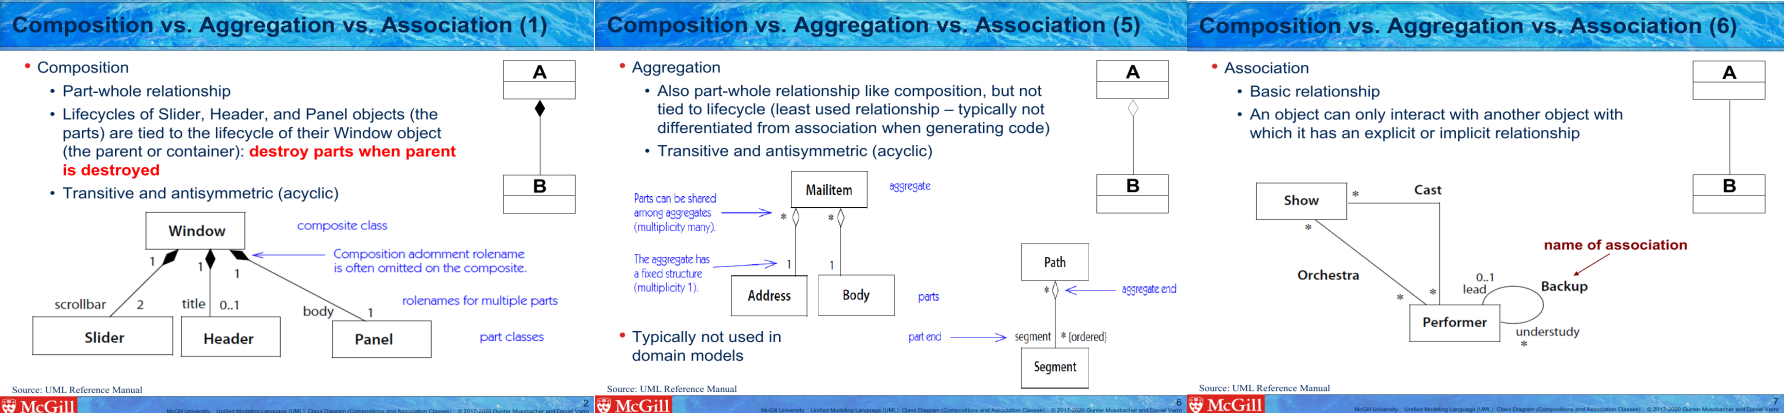
\includegraphics[width=0.9\textwidth]{images/composition_aggregation_association.png}
\end{tabular} \medskip


\subsubsection{Missing aggregation}

\noindent Level 1: Highlight solution (Relationship) \medskip

\noindent Level 2: Text response: \medskip

\begin{tabular}{|p{0.9\linewidth}}
What is the relationship between these classes?
\end{tabular} \medskip

\noindent Level 3: Parametrized response: \medskip

\begin{tabular}{|p{0.9\linewidth}}
How would you capture that a \verb|${classOne}| has a \verb|${classTwo}|?
\end{tabular} \medskip

\noindent Level 4: Resource response with Reference: \medskip

\begin{tabular}{|p{0.9\linewidth}}
Please review the _Composition vs. Aggregation vs. Association_ section of 
the \textit{UML Class Diagram lecture slides} to 
better understand these relationships and where they are used.

\\
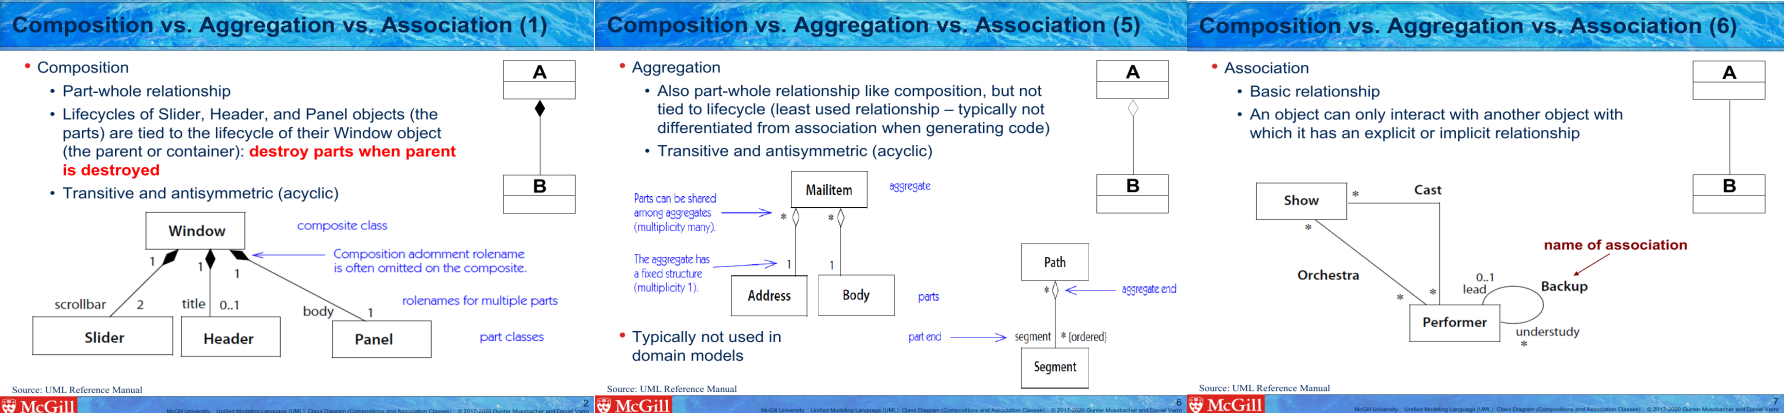
\includegraphics[width=0.9\textwidth]{images/composition_aggregation_association.png}
\end{tabular} \medskip


\subsubsection{Missing n-ary association}

\noindent Level 1: Highlight solution  \medskip

\noindent Level 2: Text response: \medskip

\begin{tabular}{|p{0.9\linewidth}}
What is the relationship between these classes?
\end{tabular} \medskip

\noindent Level 3: Parametrized response: \medskip

\begin{tabular}{|p{0.9\linewidth}}
How would you capture the relationship between \verb|${classOne}|, \verb|${classTwo}|, [and] \verb|${classThree}|[, [and] \verb|${classFour}|[, [and] \verb|${classFive}|]]?
\end{tabular} \medskip

\noindent Level 4: Resource response with Reference: \medskip

\begin{tabular}{|p{0.9\linewidth}}
Please review the _Composition vs. Aggregation vs. Association_ section of 
the \textit{UML Class Diagram lecture slides} to 
better understand these relationships and where they are used.

\\
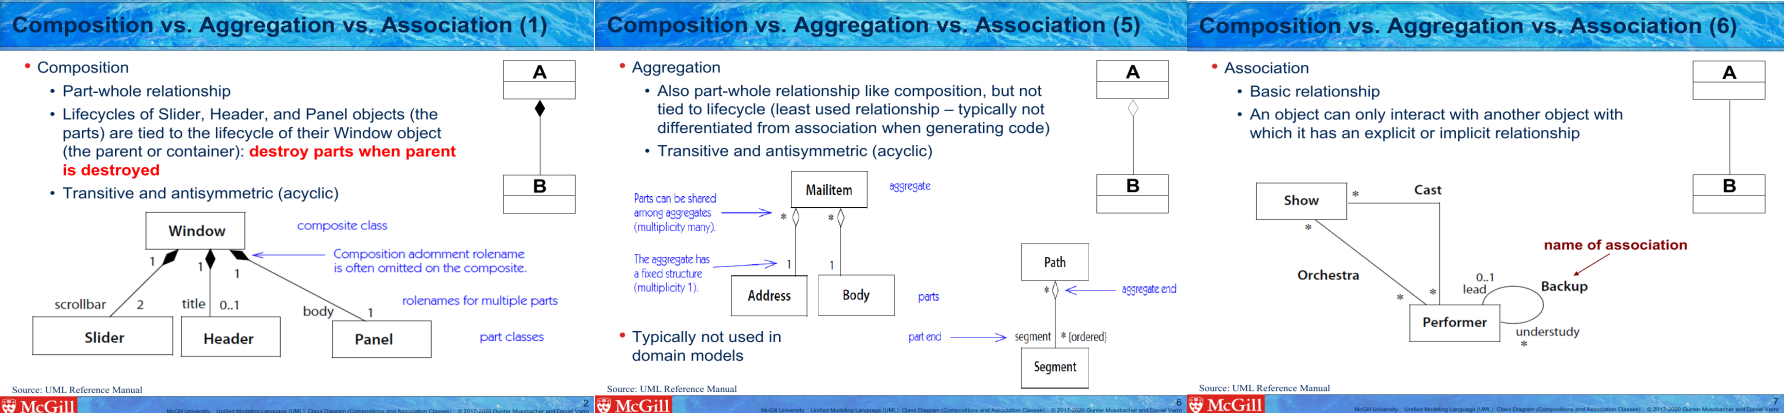
\includegraphics[width=0.9\textwidth]{images/composition_aggregation_association.png}
\end{tabular} \medskip


\subsubsection{Using attribute instead of association}

\noindent Level 1: Highlight solution (Relationship) \medskip

\noindent Level 2: Text response: \medskip

\begin{tabular}{|p{0.9\linewidth}}
Remember that attributes are simple pieces of data.
\end{tabular} \medskip

\noindent Level 3: Parametrized response: \medskip

\begin{tabular}{|p{0.9\linewidth}}
\verb|${stud_attr}| should be its own class.
\end{tabular} \medskip

\noindent Level 4: Resource response with List multiple-choice quiz: \medskip

\begin{tabular}{|p{0.9\linewidth}}

Pick the class(es) modeled correctly in Umple.

\begin{itemize}
    \item[$\square$] class BankAccount \{ Client client; \}
    \item[$\boxtimes$] class BankAccount \{ * -- 1..2 Client clients; \}; class Client \{\}
    \item[$\square$] class BankAccount \{ 1..2 -- * Client clients; \}; class Client \{\}
    \item[$\square$] class Loan \{ libraryPatron; \}
\end{itemize}

\end{tabular} \medskip

\noindent Level 5: Resource response with Reference: \medskip

\begin{tabular}{|p{0.9\linewidth}}
Please review the _Composition vs. Aggregation vs. Association_ section of 
the \textit{UML Class Diagram lecture slides} to 
better understand these relationships and where they are used.

\\
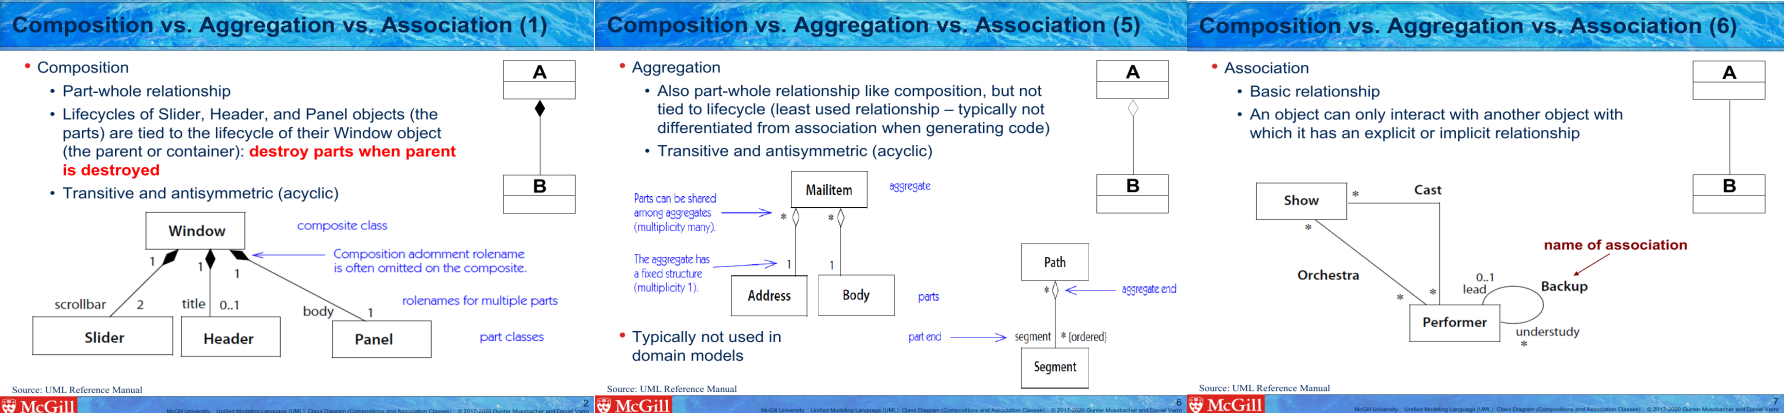
\includegraphics[width=0.9\textwidth]{images/composition_aggregation_association.png}
\end{tabular} \medskip


\subsection{Extra association mistakes}

\subsubsection{Extra association}

\noindent Level 1: Highlight solution (Relationship) \medskip

\noindent Level 2: Text response: \medskip

\begin{tabular}{|p{0.9\linewidth}}
Is this association really necessary?
\end{tabular} \medskip

\noindent Level 3: Parametrized response: \medskip

\begin{tabular}{|p{0.9\linewidth}}
The relationship between \verb|${stud_rel.end0}| and \verb|${stud_rel.end1}| is not expressed in the problem description.
\end{tabular} \medskip

\noindent Level 4: Resource response with List multiple-choice quiz: \medskip

\begin{tabular}{|p{0.9\linewidth}}

Find the redundant association(s) in this class diagram:

\\
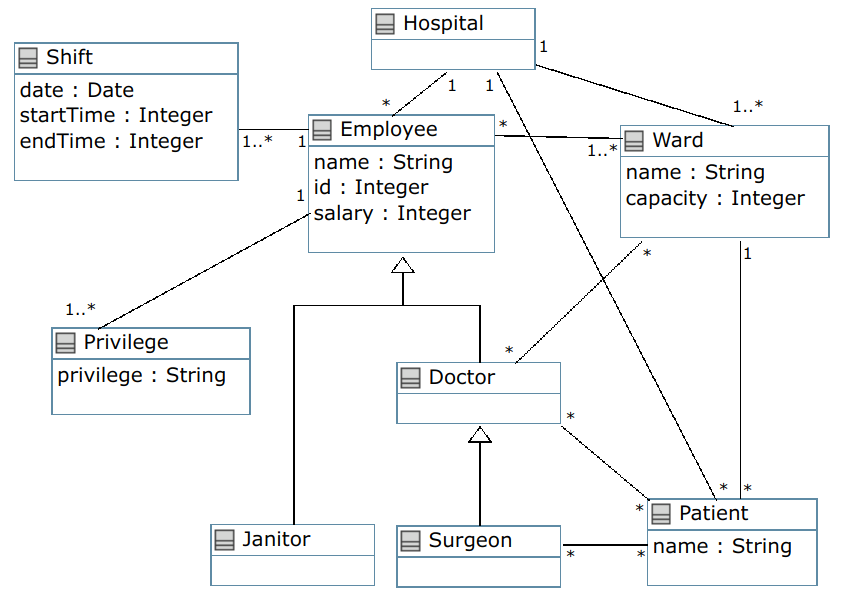
\includegraphics[width=0.6\textwidth]{images/hospital_cdm_extra_assocs.png}

\begin{itemize}
    \item[$\boxtimes$] Hospital -- Patient
    \item[$\square$] Hospital -- Employee
    \item[$\boxtimes$] Patient -- Surgeon
    \item[$\boxtimes$] Doctor -- Ward
    \item[$\square$] Hospital -- Ward
\end{itemize}

\end{tabular} \medskip

\noindent Level 5: Resource response with Reference: \medskip

\begin{tabular}{|p{0.9\linewidth}}
Please review the \textit{domain modeling lecture} to know which concepts should be a part of a domain model.
\end{tabular} \medskip


\subsubsection{Extra aggregation}

\noindent Level 1: Highlight solution (Relationship) \medskip

\noindent Level 2: Text response: \medskip

\begin{tabular}{|p{0.9\linewidth}}
Is this aggregation really necessary?
\end{tabular} \medskip

\noindent Level 3: Parametrized response: \medskip

\begin{tabular}{|p{0.9\linewidth}}
The relationship between \verb|${stud_rel.end0}| and \verb|${stud_rel.end1}| is redundant.
\end{tabular} \medskip

\noindent Level 4: Resource response with Reference: \medskip

\begin{tabular}{|p{0.9\linewidth}}
Please review the \textit{domain modeling lecture} to know which concepts should be a part of a domain model.
\end{tabular} \medskip


\subsubsection{Extra n-ary association}

\noindent Level 1: Highlight solution  \medskip

\noindent Level 2: Text response: \medskip

\begin{tabular}{|p{0.9\linewidth}}
Is this association really necessary?
\end{tabular} \medskip

\noindent Level 3: Text response: \medskip

\begin{tabular}{|p{0.9\linewidth}}
The relationship between the highlighted classes is redundant.
\end{tabular} \medskip

\noindent Level 4: Resource response with Reference: \medskip

\begin{tabular}{|p{0.9\linewidth}}
Please review the \textit{domain modeling lecture} to know which concepts should be a part of a domain model.
\end{tabular} \medskip


\subsection{Multiplicity mistakes}

\subsubsection{Infinite recursive dependency}

\noindent Level 1: Highlight solution (Relationship) \medskip

\noindent Level 2: Text response: \medskip

\begin{tabular}{|p{0.9\linewidth}}
Double check this relationship.
\end{tabular} \medskip

\noindent Level 3: Text response: \medskip

\begin{tabular}{|p{0.9\linewidth}}
The multiplicit(y$|$ies) for this relationship (is$|$are) incorrect.
\end{tabular} \medskip

\noindent Level 4: Parametrized response: \medskip

\begin{tabular}{|p{0.9\linewidth}}
Does every \verb|${className}| have exactly \verb|${wrongMultiplicity}| \verb|${rolename}|[s]?
\end{tabular} \medskip

\noindent Level 5: Resource response with List multiple-choice quiz: \medskip

\begin{tabular}{|p{0.9\linewidth}}

Given the following class diagram modeled in Umple, select the correct answer(s).

class Employee \{ 1 supervisor -- * Employee employees; \}

\begin{itemize}
    \item[$\square$] The class diagram is correct.
    \item[$\square$] The class diagram is incorrect, because some Employees do not oversee any other Employees.
    \item[$\square$] The "employees" multiplicity should be 1..* instead of *.
    \item[$\boxtimes$] The class diagram is incorrect, because at least one Employee cannot have a supervisor, otherwise an infinite recursive dependency will occur.
\end{itemize}

\end{tabular} \medskip

\noindent Level 6: Resource response with Reference: \medskip

\begin{tabular}{|p{0.9\linewidth}}
Please review the \textit{multiplicities} part of the Class Diagram lecture.
\end{tabular} \medskip


\subsubsection{Wrong multiplicity}

\noindent Level 1: Highlight solution (Relationship) \medskip

\noindent Level 2: Text response: \medskip

\begin{tabular}{|p{0.9\linewidth}}
Double check this association.
\end{tabular} \medskip

\noindent Level 3: Text response: \medskip

\begin{tabular}{|p{0.9\linewidth}}
The multiplicit(y$|$ies) for this association (is$|$are) incorrect.
\end{tabular} \medskip

\noindent Level 4: Parametrized response: \medskip

\begin{tabular}{|p{0.9\linewidth}}
How many \verb|${stud_assocend.end0}|'s does a \verb|${stud_assocend.end1}| have?[ And how many \verb|${stud_assocend.end1}|'s does \verb|${stud_assocend.end0}| have?]
\end{tabular} \medskip

\noindent Level 5: Resource response with List multiple-choice quiz: \medskip

\begin{tabular}{|p{0.9\linewidth}}

Pick the association(s) with correct multiplicities:

\begin{itemize}
    \item[$\square$] 1 EmployeeRole -- 1 Person;
    \item[$\boxtimes$] * Episode -- 1 TvSeries;
    \item[$\square$] * Bank -- 1 Client;
    \item[$\square$] * Client -- 1 BankAccount;
    \item[$\boxtimes$] 0..2 Loan -- 1 Client;
    \item[$\boxtimes$] * Person -- 1 EmployeeRole;
    \item[$\square$] * EmployeeRole -- 1 Person;
\end{itemize}

\end{tabular} \medskip

\noindent Level 6: Resource response with Reference: \medskip

\begin{tabular}{|p{0.9\linewidth}}
Please review the \textit{multiplicities} part of the Class Diagram lecture.
\end{tabular} \medskip


\subsubsection{Missing multiplicity}

\noindent Level 1: Highlight solution  \medskip

\noindent Level 2: Text response: \medskip

\begin{tabular}{|p{0.9\linewidth}}
Double check this association.
\end{tabular} \medskip

\noindent Level 3: Text response: \medskip

\begin{tabular}{|p{0.9\linewidth}}
The multiplicit(y$|$ies) for this association (is$|$are) missing.
\end{tabular} \medskip

\noindent Level 4: Parametrized response: \medskip

\begin{tabular}{|p{0.9\linewidth}}
How many \verb|${class1}|'s does a \verb|${class2}| have? [And how many \verb|${class2}|'s does \verb|${class1}| have?]
\end{tabular} \medskip

\noindent Level 5: Resource response with List multiple-choice quiz: \medskip

\begin{tabular}{|p{0.9\linewidth}}

Pick the association(s) with correct multiplicities:

\begin{itemize}
    \item[$\square$] 1 EmployeeRole -- 1 Person;
    \item[$\boxtimes$] * Episode -- 1 TvSeries;
    \item[$\square$] * Bank -- 1 Client;
    \item[$\square$] * Client -- 1 BankAccount;
    \item[$\boxtimes$] 0..2 Loan -- 1 Client;
    \item[$\boxtimes$] * Person -- 1 EmployeeRole;
    \item[$\square$] * EmployeeRole -- 1 Person;
\end{itemize}

\end{tabular} \medskip

\noindent Level 6: Resource response with Reference: \medskip

\begin{tabular}{|p{0.9\linewidth}}
Please review the \textit{multiplicities} part of the Class Diagram lecture.
\end{tabular} \medskip


\subsection{Role name mistakes}

\subsubsection{Missing role names}

\noindent Level 1: Highlight solution (Relationship) \medskip

\noindent Level 2: Text response: \medskip

\begin{tabular}{|p{0.9\linewidth}}
Can you model this relationship more precisely?
\end{tabular} \medskip

\noindent Level 3: Parametrized response: \medskip

\begin{tabular}{|p{0.9\linewidth}}
The multiplicities for the \verb|${stud_assocend}| association are correct, but something else is missing!
\end{tabular} \medskip

\noindent Level 4: Resource response with Reference: \medskip

\begin{tabular}{|p{0.9\linewidth}}
Can you think of appropriate \textit{role names}
for this association? Role names help identify the role a class plays in a
relationship and can be important if there is more than one relationship
between the same two classes.

\\
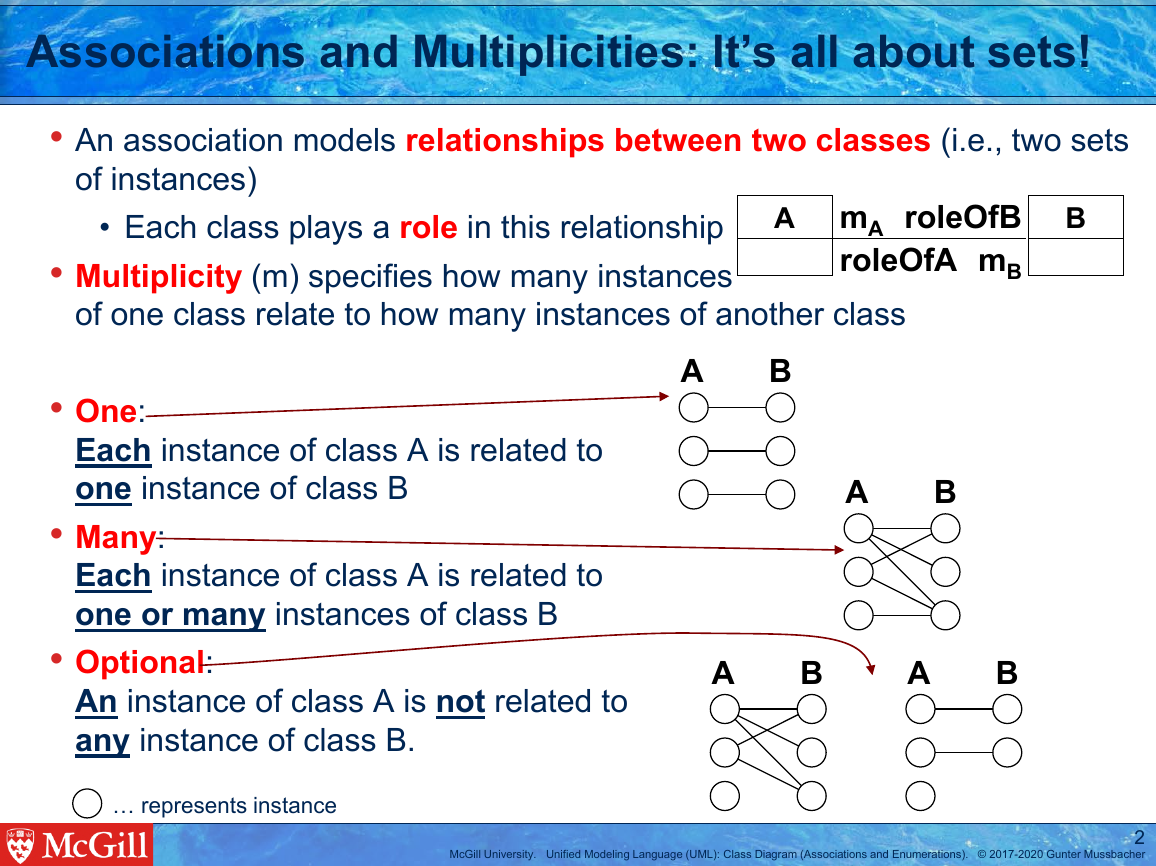
\includegraphics[width=0.6\textwidth]{images/role_name.png}

\end{tabular} \medskip


\subsubsection{Role should be static}

\noindent Level 1: Highlight solution (Relationship) \medskip

\noindent Level 2: Text response: \medskip

\begin{tabular}{|p{0.9\linewidth}}
Isn't there something special about this role name?
\end{tabular} \medskip

\noindent Level 3: Parametrized response: \medskip

\begin{tabular}{|p{0.9\linewidth}}
\verb|${stud_assocend}| should be static, because it applies to all instances of the association between \verb|${inst_assocend.end0}| and \verb|${inst_assocend.end1}|.
\end{tabular} \medskip

\noindent Level 4: Resource response with Reference: \medskip

\begin{tabular}{|p{0.9\linewidth}}
Please review the \textit{Association} part of the Class Diagram lecture.
\end{tabular} \medskip


\subsubsection{Role should not be static}

\noindent Level 1: Highlight solution (Relationship) \medskip

\noindent Level 2: Text response: \medskip

\begin{tabular}{|p{0.9\linewidth}}
Isn't there something special about this role name?
\end{tabular} \medskip

\noindent Level 3: Parametrized response: \medskip

\begin{tabular}{|p{0.9\linewidth}}
\verb|${stud_assocend}| should not be static, because it doesn't apply to all instances of the association between \verb|${inst_assocend.end0}| and \verb|${inst_assocend.end1}|.
\end{tabular} \medskip

\noindent Level 4: Resource response with Reference: \medskip

\begin{tabular}{|p{0.9\linewidth}}
Please review the \textit{Association} part of the Class Diagram lecture.
\end{tabular} \medskip


\subsubsection{Bad role name spelling}

\noindent Level 1: Highlight solution (Relationship) \medskip

\noindent Level 2: Text response: \medskip

\begin{tabular}{|p{0.9\linewidth}}
Double check this role name
\end{tabular} \medskip

\noindent Level 3: Parametrized response: \medskip

\begin{tabular}{|p{0.9\linewidth}}
\verb|${stud_assocend}| is misspelled.[ Use the same spelling as the problem description.]
\end{tabular} \medskip

\noindent Level 4: Resource response with Reference: \medskip

\begin{tabular}{|p{0.9\linewidth}}
Please review the \textit{Association} and \textit{Noun Analysis} parts of the Class Diagram lecture.
\end{tabular} \medskip


\subsubsection{Representing an action with an association}

\noindent Level 1: Highlight solution (Relationship) \medskip

\noindent Level 2: Text response: \medskip

\begin{tabular}{|p{0.9\linewidth}}
Is this the best role name to use here?
\end{tabular} \medskip

\noindent Level 3: Parametrized response: \medskip

\begin{tabular}{|p{0.9\linewidth}}
The \verb|${stud_assocend}| role name represents an action, which is not correct.[ Use \verb|${inst_assocend}| instead.]
\end{tabular} \medskip

\noindent Level 4: Resource response with Reference: \medskip

\begin{tabular}{|p{0.9\linewidth}}
Please review the \textit{Association} and \textit{Noun Analysis} parts of the Class Diagram lecture.
\end{tabular} \medskip


\subsubsection{Wrong role name but correct association}

\noindent Level 1: Highlight solution (Relationship) \medskip

\noindent Level 2: Text response: \medskip

\begin{tabular}{|p{0.9\linewidth}}
Double check this role name.
\end{tabular} \medskip

\noindent Level 3: Parametrized response: \medskip

\begin{tabular}{|p{0.9\linewidth}}
The \verb|${stud_assocend}| role name is not correct.
\end{tabular} \medskip

\noindent Level 4: Parametrized response: \medskip

\begin{tabular}{|p{0.9\linewidth}}
The \verb|${stud_assocend}| role name should be changed to \verb|${inst_assocend}|.
\end{tabular} \medskip

\noindent Level 5: Resource response with Reference: \medskip

\begin{tabular}{|p{0.9\linewidth}}
Can you think of appropriate \textit{role names}
for this association? Role names help identify the role a class plays in a
relationship and can be important if there is more than one relationship
between the same two classes.

\\
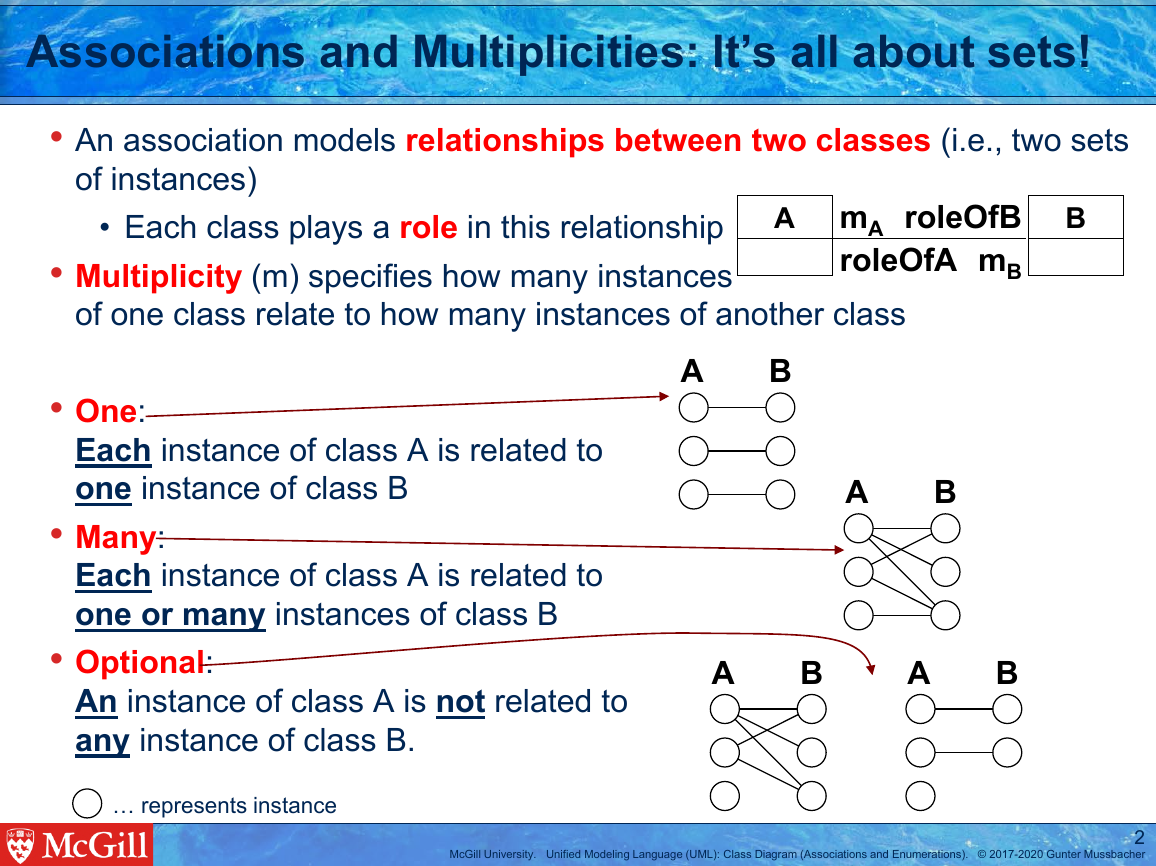
\includegraphics[width=0.6\textwidth]{images/role_name.png}

\end{tabular} \medskip


\subsection{Association type mistakes}

\subsubsection{Using aggregation instead of association}

\noindent Level 1: Highlight solution  \medskip

\noindent Level 2: Text response: \medskip

\begin{tabular}{|p{0.9\linewidth}}
What is the relationship between these two concepts?
\end{tabular} \medskip

\noindent Level 3: Parametrized response: \medskip

\begin{tabular}{|p{0.9\linewidth}}
The relationship between \verb|${containedClass}| and \verb|${containerClass}| can be modeled with a simple association.
\end{tabular} \medskip

\noindent Level 4: Resource response with Reference: \medskip

\begin{tabular}{|p{0.9\linewidth}}
Please review the _Composition vs. Aggregation vs. Association_ section of 
the \textit{UML Class Diagram lecture slides} to 
better understand these relationships and where they are used.

\\
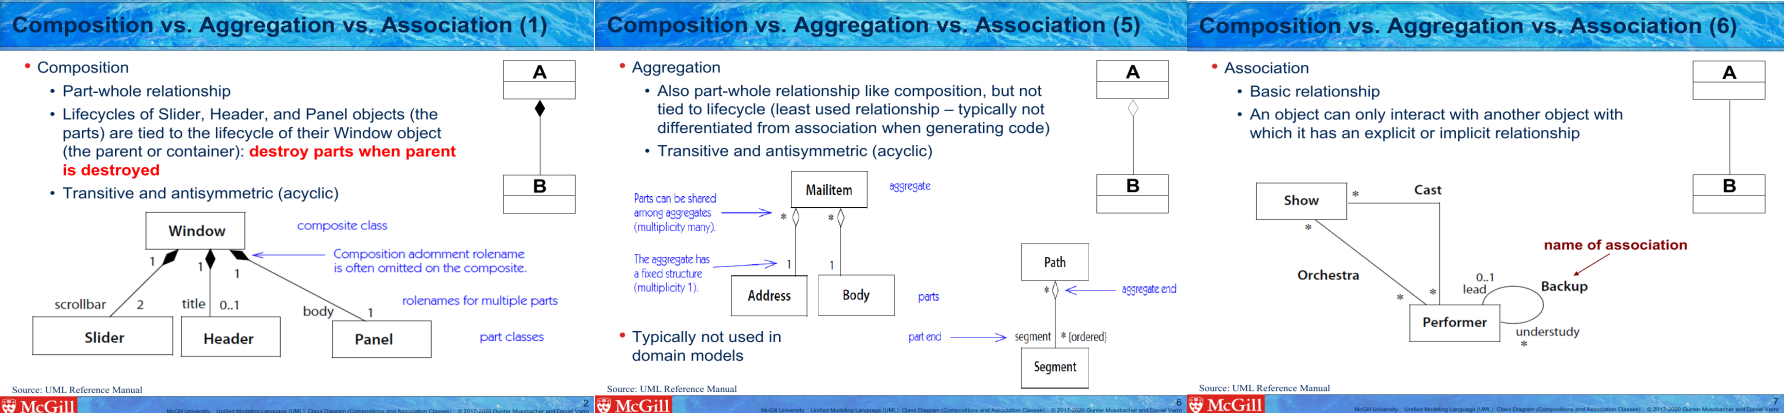
\includegraphics[width=0.9\textwidth]{images/composition_aggregation_association.png}
\end{tabular} \medskip


\subsubsection{Using composition instead of association}

\noindent Level 1: Highlight solution (Relationship) \medskip

\noindent Level 2: Text response: \medskip

\begin{tabular}{|p{0.9\linewidth}}
What is the relationship between these two concepts?
\end{tabular} \medskip

\noindent Level 3: Parametrized response: \medskip

\begin{tabular}{|p{0.9\linewidth}}
Why is \verb|${incorrectlyContainedClass}| contained in \verb|${containerClass}|?
\end{tabular} \medskip

\noindent Level 4: Resource response with Reference: \medskip

\begin{tabular}{|p{0.9\linewidth}}
Please review the _Composition vs. Aggregation vs. Association_ section of 
the \textit{UML Class Diagram lecture slides} to 
better understand these relationships and where they are used.

\\
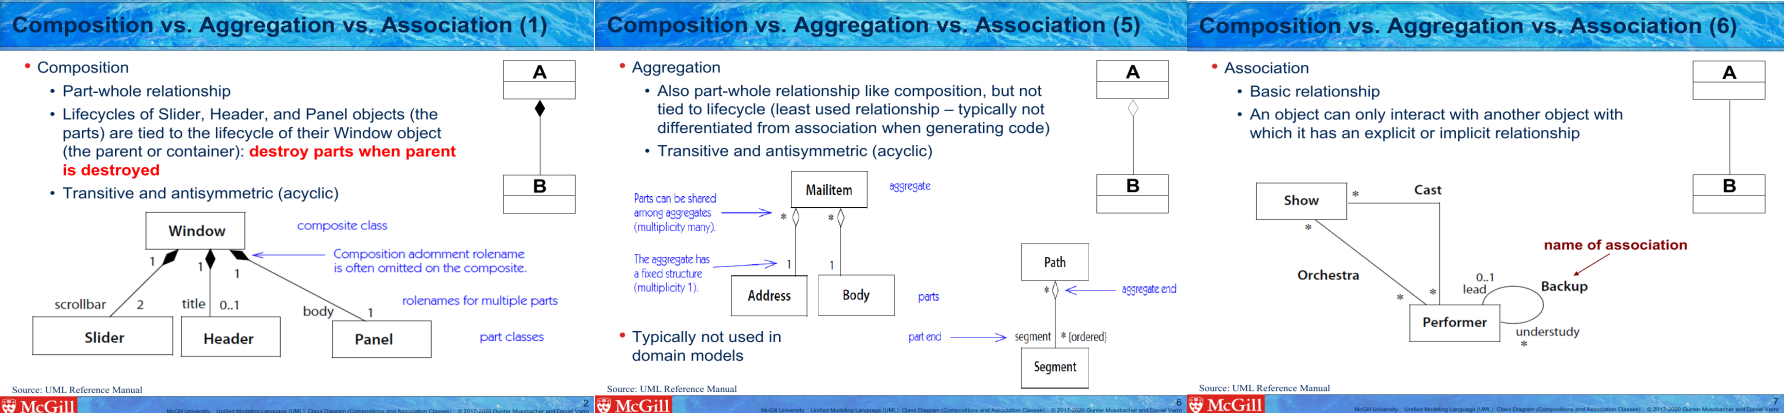
\includegraphics[width=0.9\textwidth]{images/composition_aggregation_association.png}
\end{tabular} \medskip


\subsubsection{Using directed relationship instead of undirected relationship}

\noindent Level 1: Highlight solution (Relationship) \medskip

\noindent Level 2: Text response: \medskip

\begin{tabular}{|p{0.9\linewidth}}
Why is navigation restricted for this relationship?
\end{tabular} \medskip

\noindent Level 3: Parametrized response: \medskip

\begin{tabular}{|p{0.9\linewidth}}
The relationship between \verb|${stud_assocend.end0}| and \verb|${stud_assocend.end1}| should be undirected.
\end{tabular} \medskip

\noindent Level 4: Resource response with Reference: \medskip

\begin{tabular}{|p{0.9\linewidth}}
Please review the _Directionality in Associations_ section of the \textit{UML Class Diagram lecture slides}
\end{tabular} \medskip


\subsubsection{Using undirected relationship instead of directed relationship}

\noindent Level 1: Highlight solution (Relationship) \medskip

\noindent Level 2: Parametrized response: \medskip

\begin{tabular}{|p{0.9\linewidth}}
Does \verb|${targetClass}| need to know about \verb|${sourceClass}|?
\end{tabular} \medskip

\noindent Level 3: Parametrized response: \medskip

\begin{tabular}{|p{0.9\linewidth}}
The relationship between \verb|${classOne}| and \verb|${classTwo}| should be directed[ from \verb|${classOne}| to \verb|${classTwo}|].
\end{tabular} \medskip

\noindent Level 4: Resource response with Reference: \medskip

\begin{tabular}{|p{0.9\linewidth}}
Please review the _Directionality in Associations_ section of the \textit{UML Class Diagram lecture slides}
\end{tabular} \medskip


\subsubsection{Using composition instead of aggregation}

\noindent Level 1: Highlight solution (Relationship) \medskip

\noindent Level 2: Text response: \medskip

\begin{tabular}{|p{0.9\linewidth}}
Is this the best relationship to use here?
\end{tabular} \medskip

\noindent Level 3: Parametrized response: \medskip

\begin{tabular}{|p{0.9\linewidth}}
The composition between \verb|${stud_assocend.end0}| and \verb|${stud_assocend.end1}| is better modeled using aggregation.
\end{tabular} \medskip

\noindent Level 4: Resource response with Reference: \medskip

\begin{tabular}{|p{0.9\linewidth}}
Please review the _Composition vs. Aggregation vs. Association_ section of 
the \textit{UML Class Diagram lecture slides} to 
better understand these relationships and where they are used.

\\
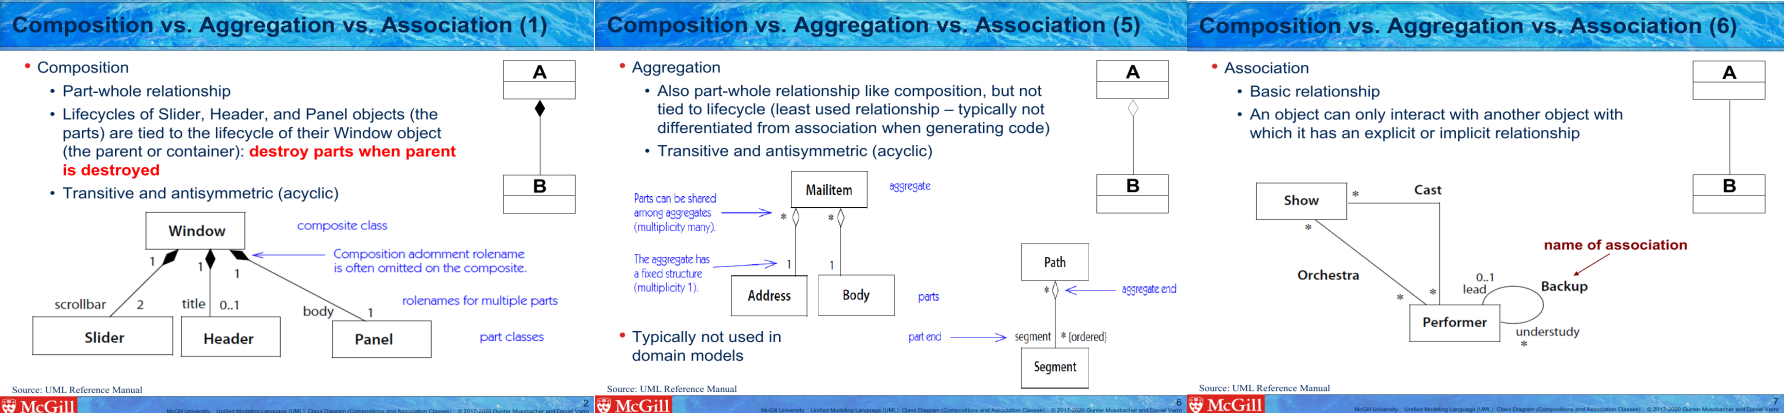
\includegraphics[width=0.9\textwidth]{images/composition_aggregation_association.png}
\end{tabular} \medskip


\subsubsection{Using binary association instead of n-ary association}

\noindent Level 1: Highlight solution  \medskip

\noindent Level 2: Text response: \medskip

\begin{tabular}{|p{0.9\linewidth}}
Can you model this relationship more precisely?
\end{tabular} \medskip

\noindent Level 3: Parametrized response: \medskip

\begin{tabular}{|p{0.9\linewidth}}
Use a \verb|${n}|-ary association to represent this relationship.
\end{tabular} \medskip

\noindent Level 4: Resource response with Reference: \medskip

\begin{tabular}{|p{0.9\linewidth}}
Please review the \textit{Association} part of the Class Diagram lecture.
\end{tabular} \medskip


\subsubsection{Using n-ary association instead of binary association}

\noindent Level 1: Highlight solution  \medskip

\noindent Level 2: Text response: \medskip

\begin{tabular}{|p{0.9\linewidth}}
Can you model this relationship more precisely?
\end{tabular} \medskip

\noindent Level 3: Text response: \medskip

\begin{tabular}{|p{0.9\linewidth}}
Use a binary association to represent this relationship.
\end{tabular} \medskip

\noindent Level 4: Resource response with Reference: \medskip

\begin{tabular}{|p{0.9\linewidth}}
Please review the \textit{Association} part of the Class Diagram lecture.
\end{tabular} \medskip


\subsubsection{Using intermediate class instead of n-ary association}

\noindent Level 1: Highlight solution  \medskip

\noindent Level 2: Text response: \medskip

\begin{tabular}{|p{0.9\linewidth}}
Can you model this relationship in a different way?
\end{tabular} \medskip

\noindent Level 3: Parametrized response: \medskip

\begin{tabular}{|p{0.9\linewidth}}
Use a \verb|${n}|-ary association to represent this relationship.
\end{tabular} \medskip

\noindent Level 4: Resource response with Reference: \medskip

\begin{tabular}{|p{0.9\linewidth}}
Please review the \textit{Association} part of the Class Diagram lecture.
\end{tabular} \medskip


\subsubsection{Using n-ary association instead of intermediate class}

\noindent Level 1: Highlight solution  \medskip

\noindent Level 2: Text response: \medskip

\begin{tabular}{|p{0.9\linewidth}}
Is this the best way to model this concept?
\end{tabular} \medskip

\noindent Level 3: Text response: \medskip

\begin{tabular}{|p{0.9\linewidth}}
Use an intermediate class instead of an n-ary association.
\end{tabular} \medskip

\noindent Level 4: Resource response with Reference: \medskip

\begin{tabular}{|p{0.9\linewidth}}
Please review the \textit{Association} part of the Class Diagram lecture.
\end{tabular} \medskip


\subsection{Association name mistakes}

\subsubsection{Missing association name}

\noindent Level 1: Highlight solution  \medskip

\noindent Level 2: Text response: \medskip

\begin{tabular}{|p{0.9\linewidth}}
Something is missing here.
\end{tabular} \medskip

\noindent Level 3: Text response: \medskip

\begin{tabular}{|p{0.9\linewidth}}
Can you give this association a name?
\end{tabular} \medskip

\noindent Level 4: Parametrized response: \medskip

\begin{tabular}{|p{0.9\linewidth}}
This association should be named \verb|${associationName}|.
\end{tabular} \medskip

\noindent Level 5: Resource response with Reference: \medskip

\begin{tabular}{|p{0.9\linewidth}}
Please review the \textit{Association} and \textit{Noun Analysis} parts of the Class Diagram lecture.
\end{tabular} \medskip


\subsubsection{Bad association name spelling}

\noindent Level 1: Highlight solution  \medskip

\noindent Level 2: Text response: \medskip

\begin{tabular}{|p{0.9\linewidth}}
Double check this association name.
\end{tabular} \medskip

\noindent Level 3: Parametrized response: \medskip

\begin{tabular}{|p{0.9\linewidth}}
\verb|${associationName}| is misspelled.[ Use the same spelling as the problem description.]
\end{tabular} \medskip

\noindent Level 4: Resource response with Reference: \medskip

\begin{tabular}{|p{0.9\linewidth}}
Please review the \textit{Association} and \textit{Noun Analysis} parts of the Class Diagram lecture.
\end{tabular} \medskip


\subsection{Association class mistakes}

\subsubsection{Missing association class}

\noindent Level 1: Highlight solution (Class) \medskip

\noindent Level 2: Text response: \medskip

\begin{tabular}{|p{0.9\linewidth}}
Can you model this relationship more precisely?
\end{tabular} \medskip

\noindent Level 3: Parametrized response: \medskip

\begin{tabular}{|p{0.9\linewidth}}
Further details of the association between \verb|${firstClass}| and \verb|${secondClass}| should be modeled with an association class.
\end{tabular} \medskip

\noindent Level 4: Resource response with Reference: \medskip

\begin{tabular}{|p{0.9\linewidth}}
Association class

\\
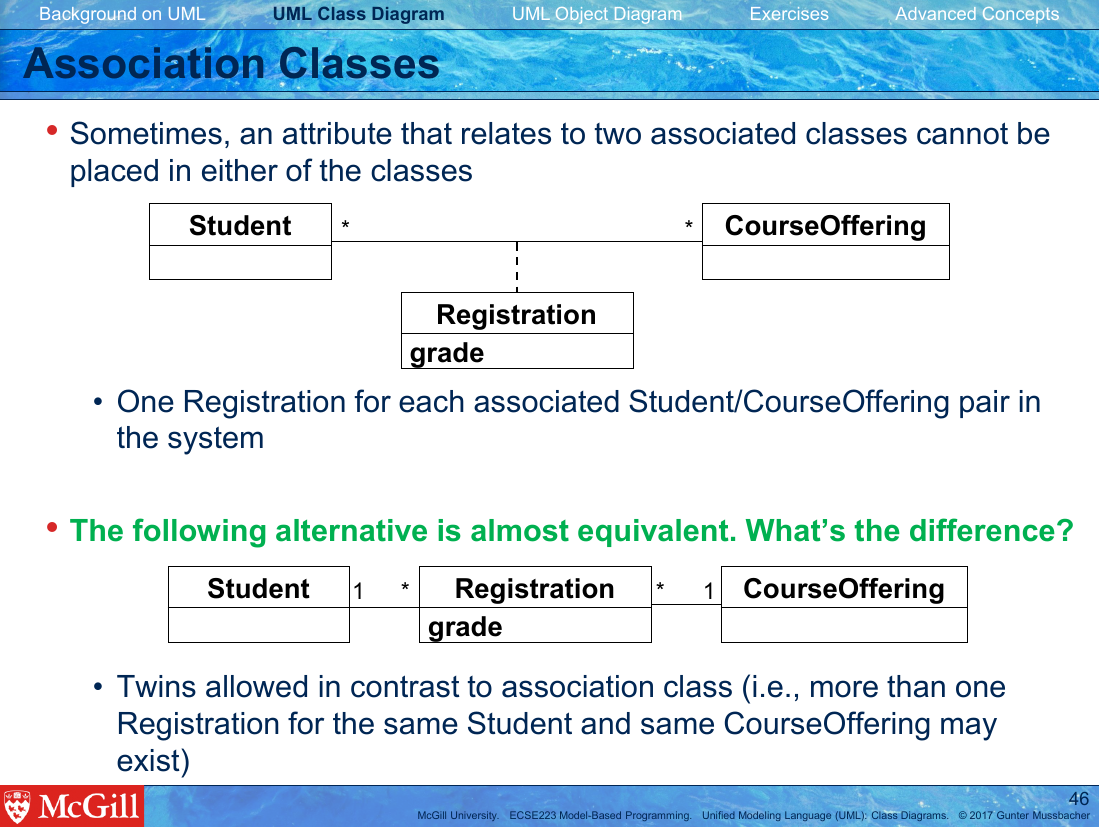
\includegraphics[width=0.6\textwidth]{images/association_class.png}
\end{tabular} \medskip


\subsubsection{Extra association class}

\noindent Level 1: Highlight solution (Class) \medskip

\noindent Level 2: Text response: \medskip

\begin{tabular}{|p{0.9\linewidth}}
Can you model this relationship in another way?
\end{tabular} \medskip

\noindent Level 3: Text response: \medskip

\begin{tabular}{|p{0.9\linewidth}}
Is using an association class the best way to model this?
\end{tabular} \medskip

\noindent Level 4: Parametrized response: \medskip

\begin{tabular}{|p{0.9\linewidth}}
Does it make sense to disallow multiple instances of the \verb|${inBetweenClass}| linking \verb|${firstClass}| and \verb|${secondClass}|?
\end{tabular} \medskip

\noindent Level 5: Parametrized response: \medskip

\begin{tabular}{|p{0.9\linewidth}}
Further details of the association between \verb|${firstClass}| and \verb|${secondClass}| should not be modeled with an association class.
\end{tabular} \medskip

\noindent Level 6: Resource response with Reference: \medskip

\begin{tabular}{|p{0.9\linewidth}}
Association class

\\
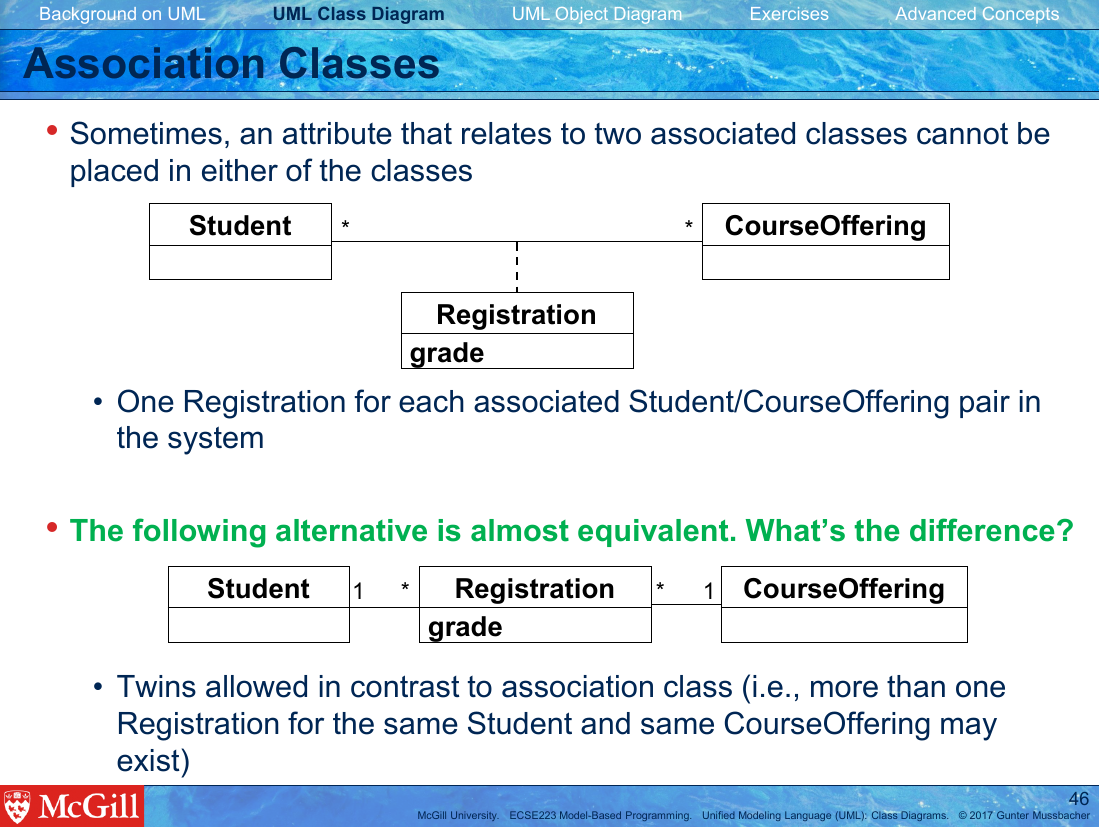
\includegraphics[width=0.6\textwidth]{images/association_class.png}
\end{tabular} \medskip


\subsubsection{Bad association class name spelling}

\noindent Level 1: Highlight solution (Class) \medskip

\noindent Level 2: Text response: \medskip

\begin{tabular}{|p{0.9\linewidth}}
Double check this association class name.
\end{tabular} \medskip

\noindent Level 3: Parametrized response: \medskip

\begin{tabular}{|p{0.9\linewidth}}
The \verb|${stud_cls}| class has a misspelled name.
\end{tabular} \medskip

\noindent Level 4: Parametrized response: \medskip

\begin{tabular}{|p{0.9\linewidth}}
The \verb|${stud_cls}| class should be changed to \verb|${inst_cls}|.
\end{tabular} \medskip

\noindent Level 5: Resource response with Reference: \medskip

\begin{tabular}{|p{0.9\linewidth}}
Please review the \textit{Classes} part of the Class Diagram lecture.
\end{tabular} \medskip


\subsubsection{Association class should be regular class}

\noindent Level 1: Highlight solution (Class) \medskip

\noindent Level 2: Text response: \medskip

\begin{tabular}{|p{0.9\linewidth}}
Can you model this relationship in another way?
\end{tabular} \medskip

\noindent Level 3: Text response: \medskip

\begin{tabular}{|p{0.9\linewidth}}
Is using an association class the best way to model this?
\end{tabular} \medskip

\noindent Level 4: Parametrized response: \medskip

\begin{tabular}{|p{0.9\linewidth}}
The \verb|${inst_cls}| class should be a regular class.
\end{tabular} \medskip

\noindent Level 5: Resource response with Reference: \medskip

\begin{tabular}{|p{0.9\linewidth}}
Association class

\\
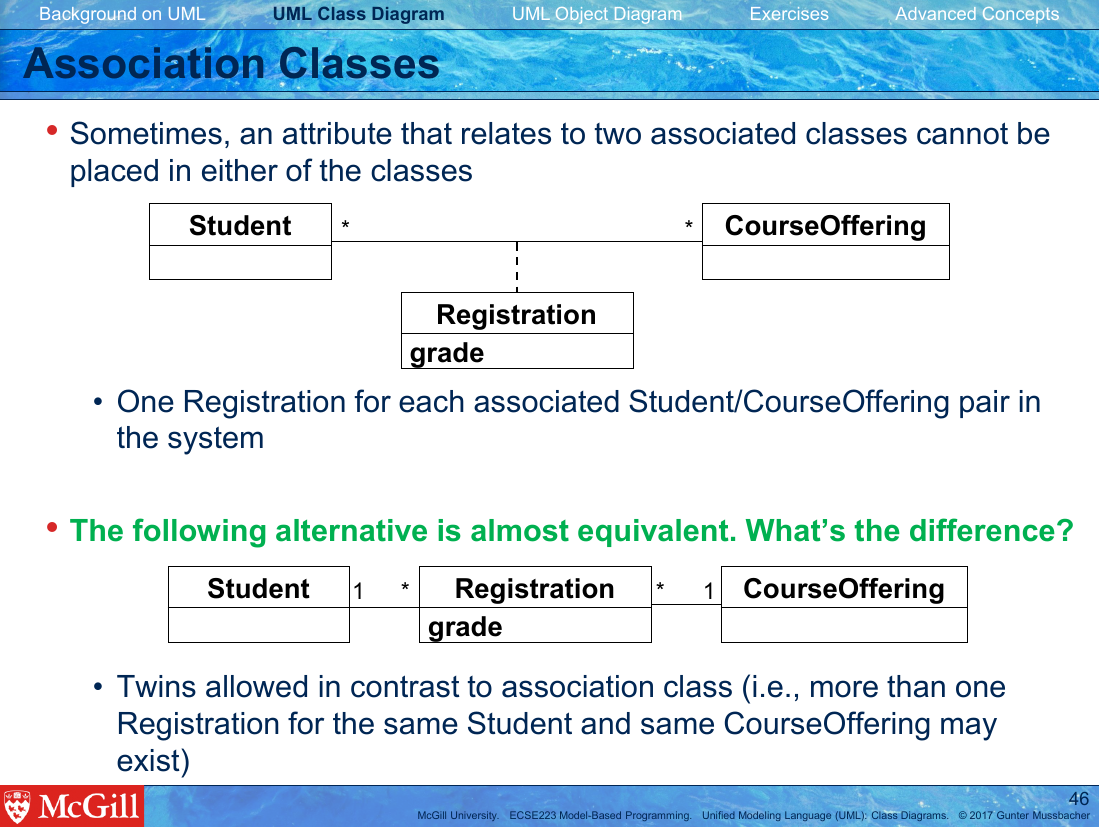
\includegraphics[width=0.6\textwidth]{images/association_class.png}
\end{tabular} \medskip


\subsubsection{Regular class should be association class}

\noindent Level 1: Highlight solution (Class) \medskip

\noindent Level 2: Text response: \medskip

\begin{tabular}{|p{0.9\linewidth}}
Can you model this relationship in another way?
\end{tabular} \medskip

\noindent Level 3: Text response: \medskip

\begin{tabular}{|p{0.9\linewidth}}
Is using a regular class the best way to model this?
\end{tabular} \medskip

\noindent Level 4: Parametrized response: \medskip

\begin{tabular}{|p{0.9\linewidth}}
The \verb|${stud_cls}| class should be an association class.
\end{tabular} \medskip

\noindent Level 5: Resource response with Reference: \medskip

\begin{tabular}{|p{0.9\linewidth}}
Association class

\\
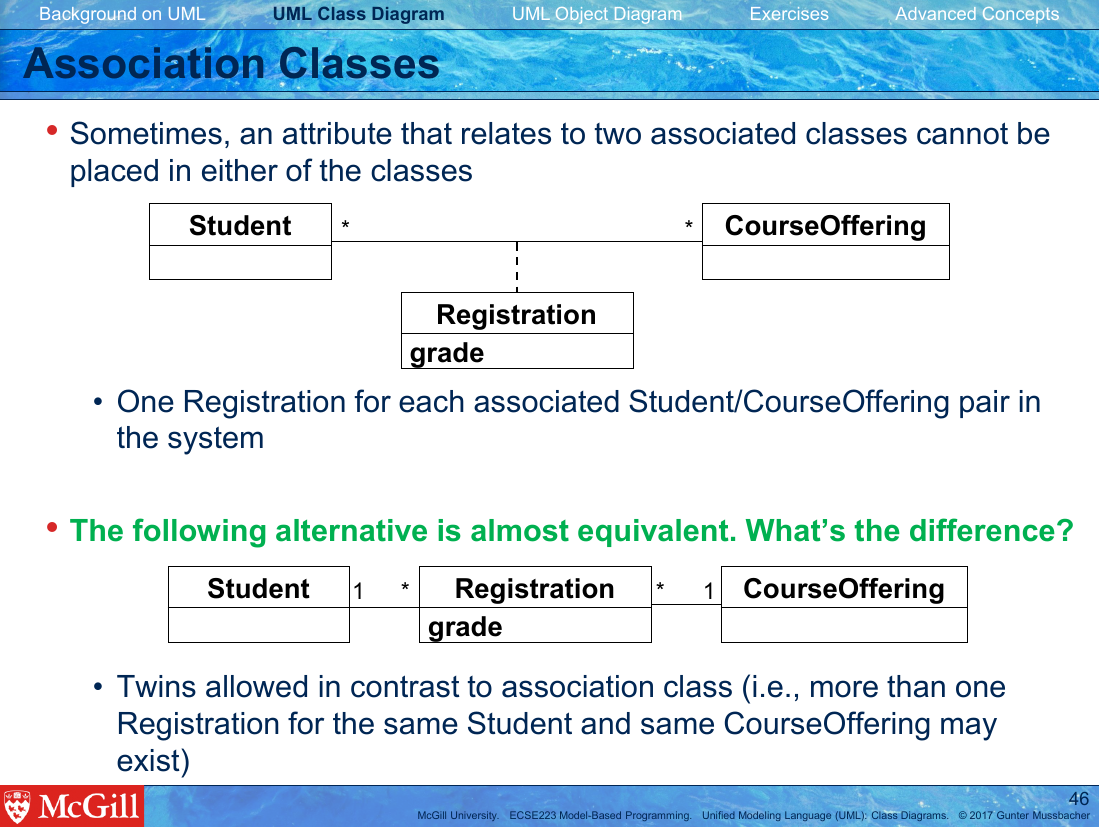
\includegraphics[width=0.6\textwidth]{images/association_class.png}
\end{tabular} \medskip


\subsection{Composition mistakes}

\subsubsection{Missing composition}

\noindent Level 1: Highlight solution (Composition) \medskip

\noindent Level 2: Text response: \medskip

\begin{tabular}{|p{0.9\linewidth}}
What is the relationship between these classes?
\end{tabular} \medskip

\noindent Level 3: Parametrized response: \medskip

\begin{tabular}{|p{0.9\linewidth}}
How would you capture that a \verb|${containerClass}| contains a \verb|${containedClass}|?
\end{tabular} \medskip

\noindent Level 4: Resource response with Reference: \medskip

\begin{tabular}{|p{0.9\linewidth}}
Please review the _Composition vs. Aggregation vs. Association_ section of 
the \textit{UML Class Diagram lecture slides} to 
better understand these relationships and where they are used.

\\
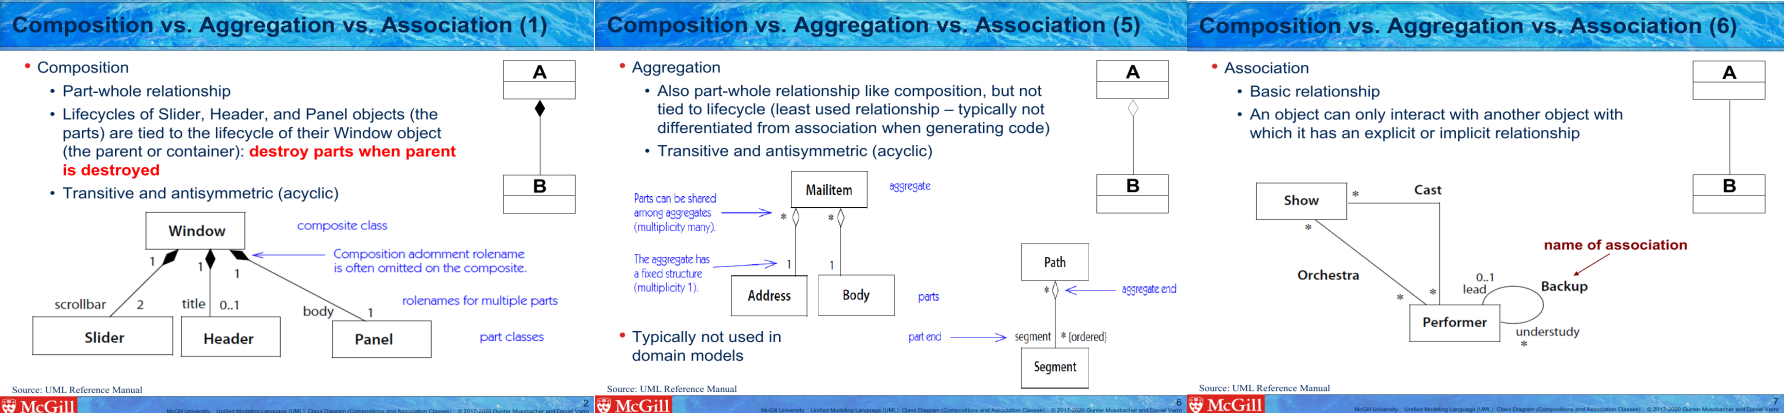
\includegraphics[width=0.9\textwidth]{images/composition_aggregation_association.png}
\end{tabular} \medskip


\subsubsection{Extra composition}

\noindent Level 1: Highlight solution (Composition) \medskip

\noindent Level 2: Text response: \medskip

\begin{tabular}{|p{0.9\linewidth}}
Is this composition really necessary?
\end{tabular} \medskip

\noindent Level 3: Parametrized response: \medskip

\begin{tabular}{|p{0.9\linewidth}}
The relationship between \verb|${stud_rel.end0}| and \verb|${stud.end1}| is not expressed in the problem description.
\end{tabular} \medskip

\noindent Level 4: Resource response with Reference: \medskip

\begin{tabular}{|p{0.9\linewidth}}
Please review the _Composition vs. Aggregation vs. Association_ section of 
the \textit{UML Class Diagram lecture slides} to 
better understand these relationships and where they are used.

\\
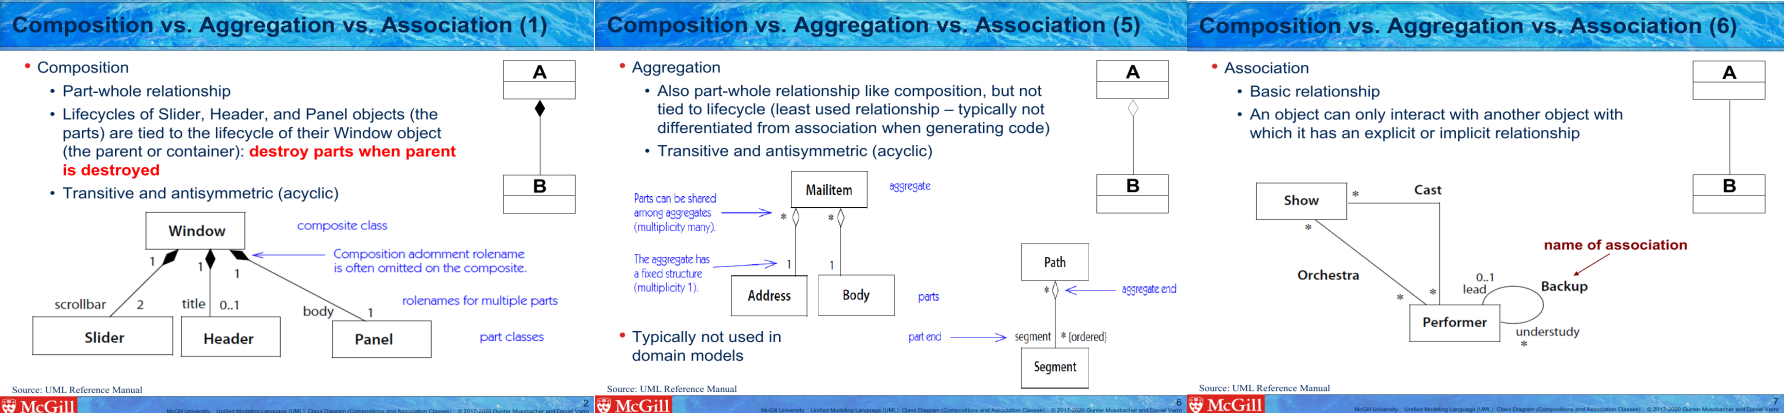
\includegraphics[width=0.9\textwidth]{images/composition_aggregation_association.png}
\end{tabular} \medskip


\subsubsection{Using association instead of aggregation}

\noindent Level 1: Highlight solution (Relationship) \medskip

\noindent Level 2: Text response: \medskip

\begin{tabular}{|p{0.9\linewidth}}
What is the relationship between these two concepts?
\end{tabular} \medskip

\noindent Level 3: Parametrized response: \medskip

\begin{tabular}{|p{0.9\linewidth}}
The relationship between \verb|${stud_assocend.end0}| and \verb|${stud_assocend.end1}| can be modeled more precisely than with a simple association.
\end{tabular} \medskip

\noindent Level 4: Resource response with Reference: \medskip

\begin{tabular}{|p{0.9\linewidth}}
Please review the _Composition vs. Aggregation vs. Association_ section of 
the \textit{UML Class Diagram lecture slides} to 
better understand these relationships and where they are used.

\\
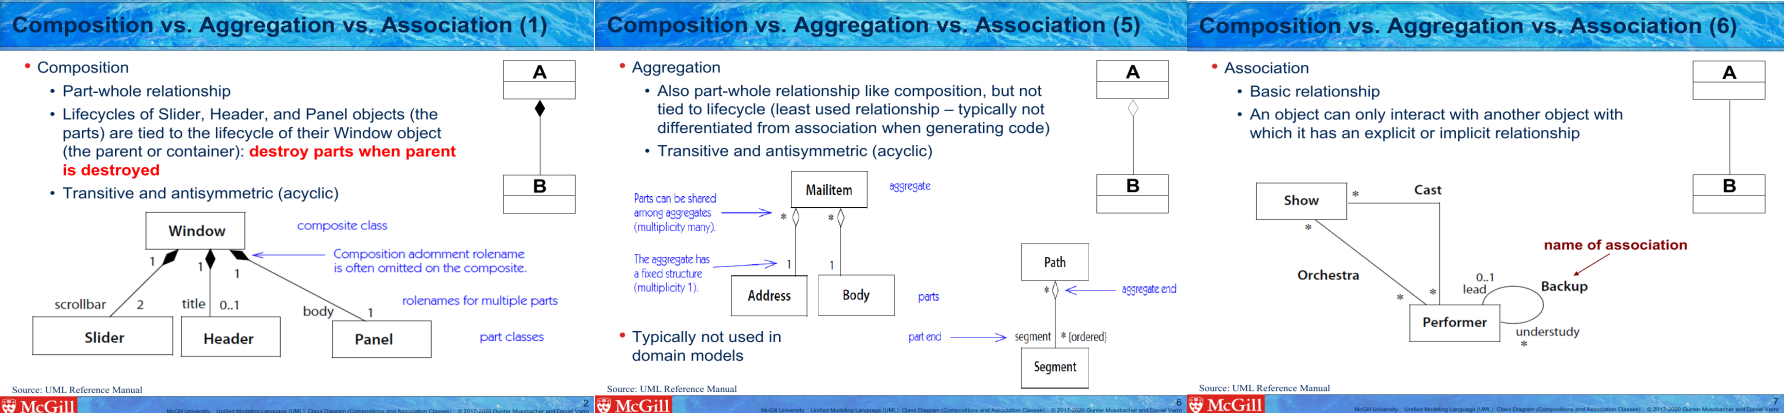
\includegraphics[width=0.9\textwidth]{images/composition_aggregation_association.png}
\end{tabular} \medskip


\subsubsection{Using association instead of composition}

\noindent Level 1: Highlight solution (Relationship) \medskip

\noindent Level 2: Text response: \medskip

\begin{tabular}{|p{0.9\linewidth}}
What is the relationship between these two concepts?
\end{tabular} \medskip

\noindent Level 3: Parametrized response: \medskip

\begin{tabular}{|p{0.9\linewidth}}
The relationship between \verb|${stud_assocend.end0}| and \verb|${stud_assocend.end1}| is more than a simple association..
\end{tabular} \medskip

\noindent Level 4: Resource response with Reference: \medskip

\begin{tabular}{|p{0.9\linewidth}}
Please review the _Composition vs. Aggregation vs. Association_ section of 
the \textit{UML Class Diagram lecture slides} to 
better understand these relationships and where they are used.

\\
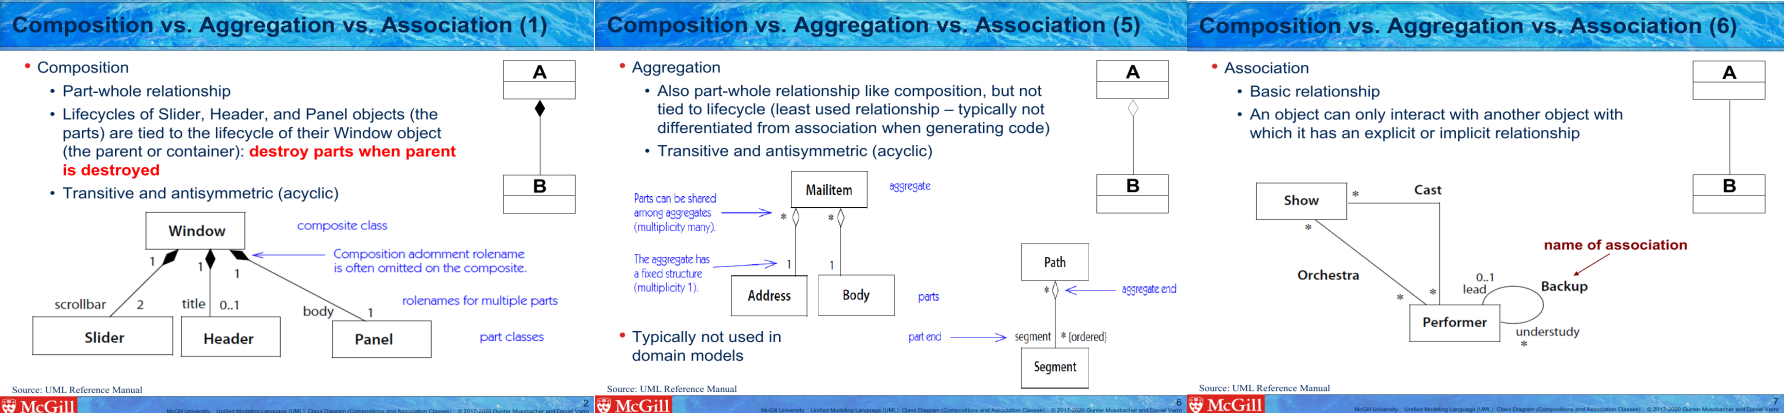
\includegraphics[width=0.9\textwidth]{images/composition_aggregation_association.png}
\end{tabular} \medskip


\subsubsection{Using aggregation instead of composition}

\noindent Level 1: Highlight solution (Relationship) \medskip

\noindent Level 2: Text response: \medskip

\begin{tabular}{|p{0.9\linewidth}}
Is this the best relationship to use here?
\end{tabular} \medskip

\noindent Level 3: Parametrized response: \medskip

\begin{tabular}{|p{0.9\linewidth}}
The relationship between \verb|${stud_assocend.end0}| and \verb|${stud_assocend.end1}| is stronger than an aggregation.
\end{tabular} \medskip

\noindent Level 4: Resource response with Reference: \medskip

\begin{tabular}{|p{0.9\linewidth}}
Please review the _Composition vs. Aggregation vs. Association_ section of 
the \textit{UML Class Diagram lecture slides} to 
better understand these relationships and where they are used.

\\
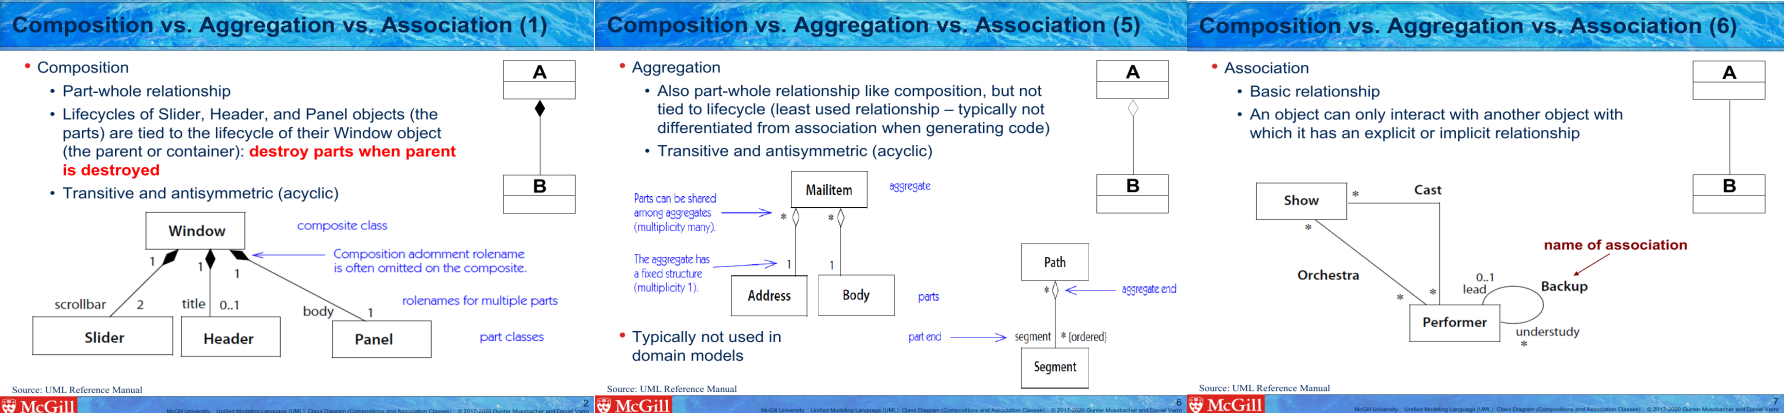
\includegraphics[width=0.9\textwidth]{images/composition_aggregation_association.png}
\end{tabular} \medskip


\subsubsection{Composed part contained in more than one parent}

\noindent Level 1: Highlight solution (Class) \medskip

\noindent Level 2: Text response: \medskip

\begin{tabular}{|p{0.9\linewidth}}
Please double-check this relationship.
\end{tabular} \medskip

\noindent Level 3: Text response: \medskip

\begin{tabular}{|p{0.9\linewidth}}
Please review the model containment hierarchy.
\end{tabular} \medskip

\noindent Level 4: Parametrized response: \medskip

\begin{tabular}{|p{0.9\linewidth}}
\verb|${incorrectlyContainedClass}| cannot be contained in more than one class.
\end{tabular} \medskip

\noindent Level 5: Resource response with Example: \medskip

\begin{tabular}{|p{0.9\linewidth}}
Observe the following domain model. Every single class except the root class is contained in the 
root class, `PISystem`.

\\
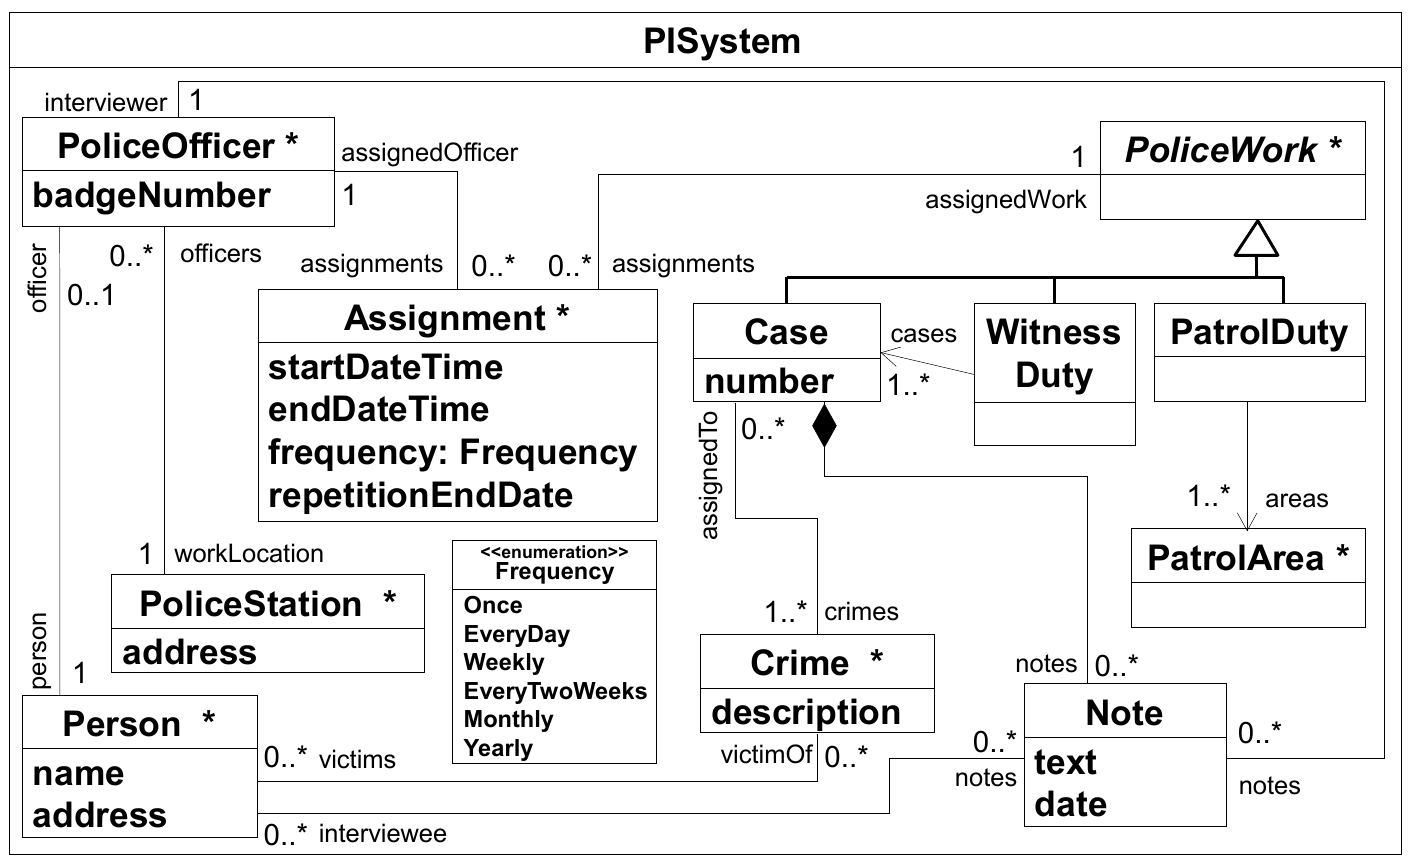
\includegraphics[width=0.6\textwidth]{images/PISystem.png}
\end{tabular} \medskip

\noindent Level 6: Resource response with List multiple-choice quiz: \medskip

\begin{tabular}{|p{0.9\linewidth}}

Which of the following compositions should be added to complete the containment tree for the
following model.

\\
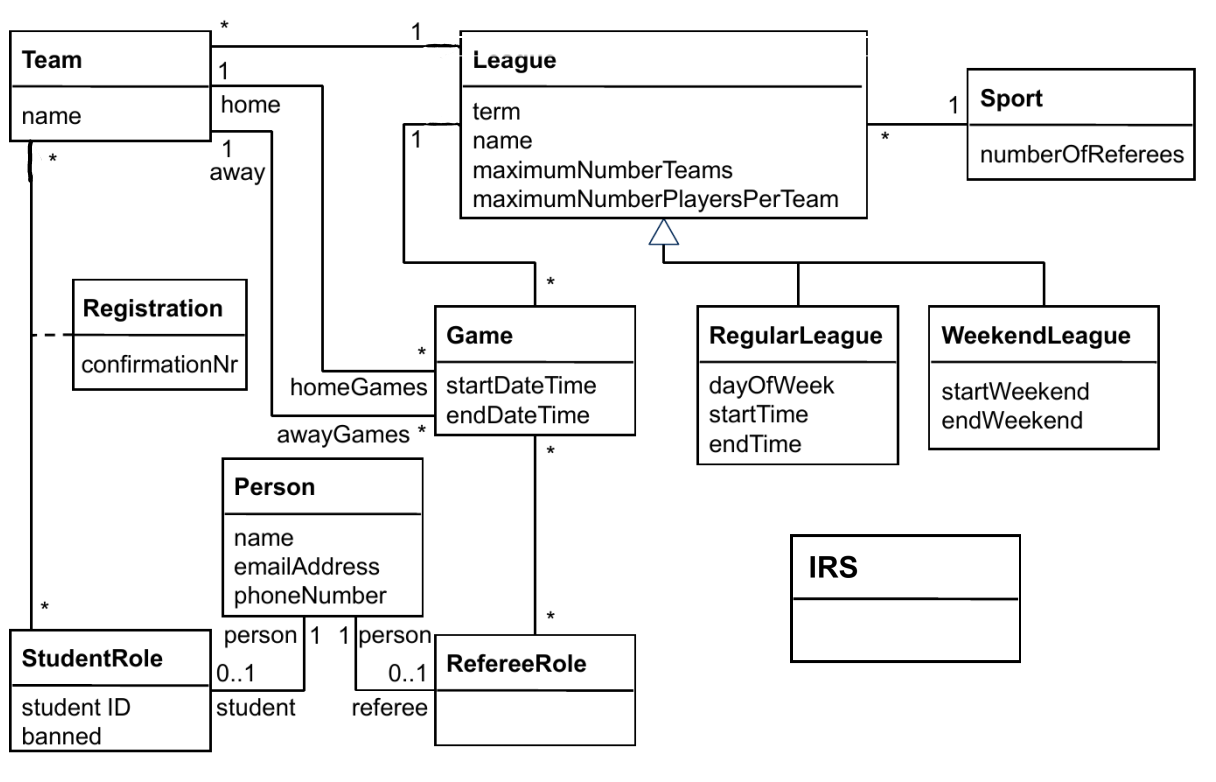
\includegraphics[width=0.6\textwidth]{images/IRS.png}

\begin{itemize}
    \item[$\boxtimes$] 1 IRS $<$@$>$- * StudentRole
    \item[$\boxtimes$] 1 IRS $<$@$>$- * Person
    \item[$\square$] 1 IRS $<$@$>$- * Game
    \item[$\boxtimes$] 1 IRS $<$@$>$- * League
    \item[$\square$] 1 IRS $<$@$>$- * RegularLeague
\end{itemize}

\end{tabular} \medskip

\noindent Level 7: Resource response with Reference: \medskip

\begin{tabular}{|p{0.9\linewidth}}
Please review the _Composition vs. Aggregation vs. Association_ section of 
the \textit{UML Class Diagram lecture slides} to 
better understand these relationships and where they are used.

\\
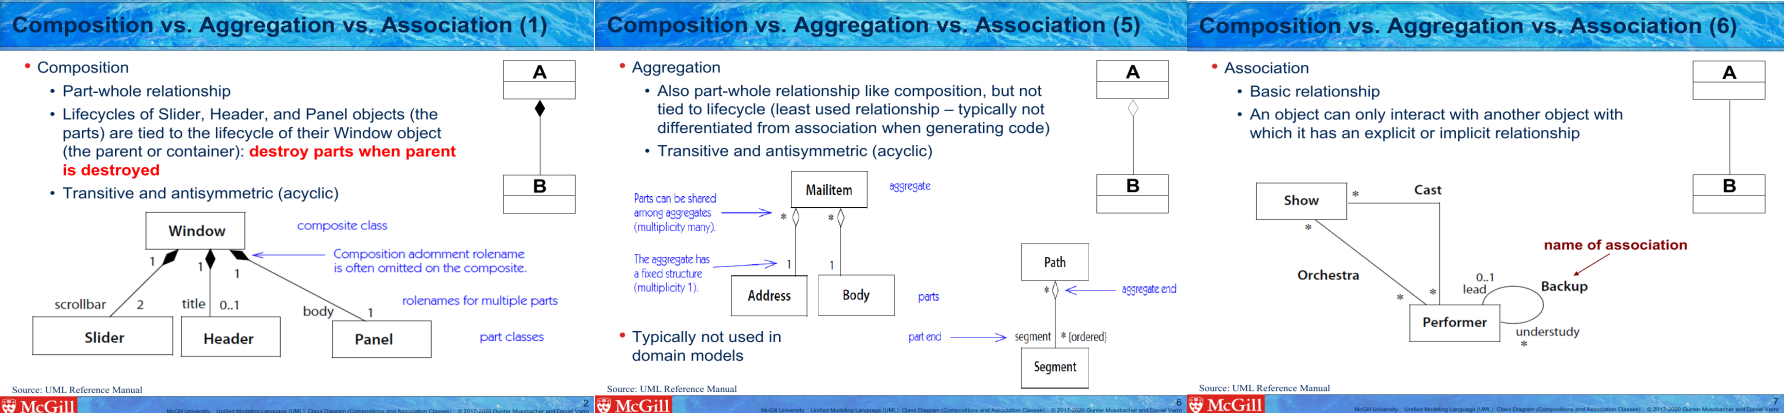
\includegraphics[width=0.9\textwidth]{images/composition_aggregation_association.png}
\end{tabular} \medskip


\subsubsection{Incomplete containment tree}

\noindent Level 1: Highlight solution (Class) \medskip

\noindent Level 2: Text response: \medskip

\begin{tabular}{|p{0.9\linewidth}}
What is the relationship between these classes?
\end{tabular} \medskip

\noindent Level 3: Parametrized response: \medskip

\begin{tabular}{|p{0.9\linewidth}}
{containedClass} is a part of \verb|${containerClass}|, so how would you model this?
\end{tabular} \medskip

\noindent Level 4: Resource response with Example: \medskip

\begin{tabular}{|p{0.9\linewidth}}
Observe the following domain model. Every single class except the root class is contained in the 
root class, `PISystem`.

\\
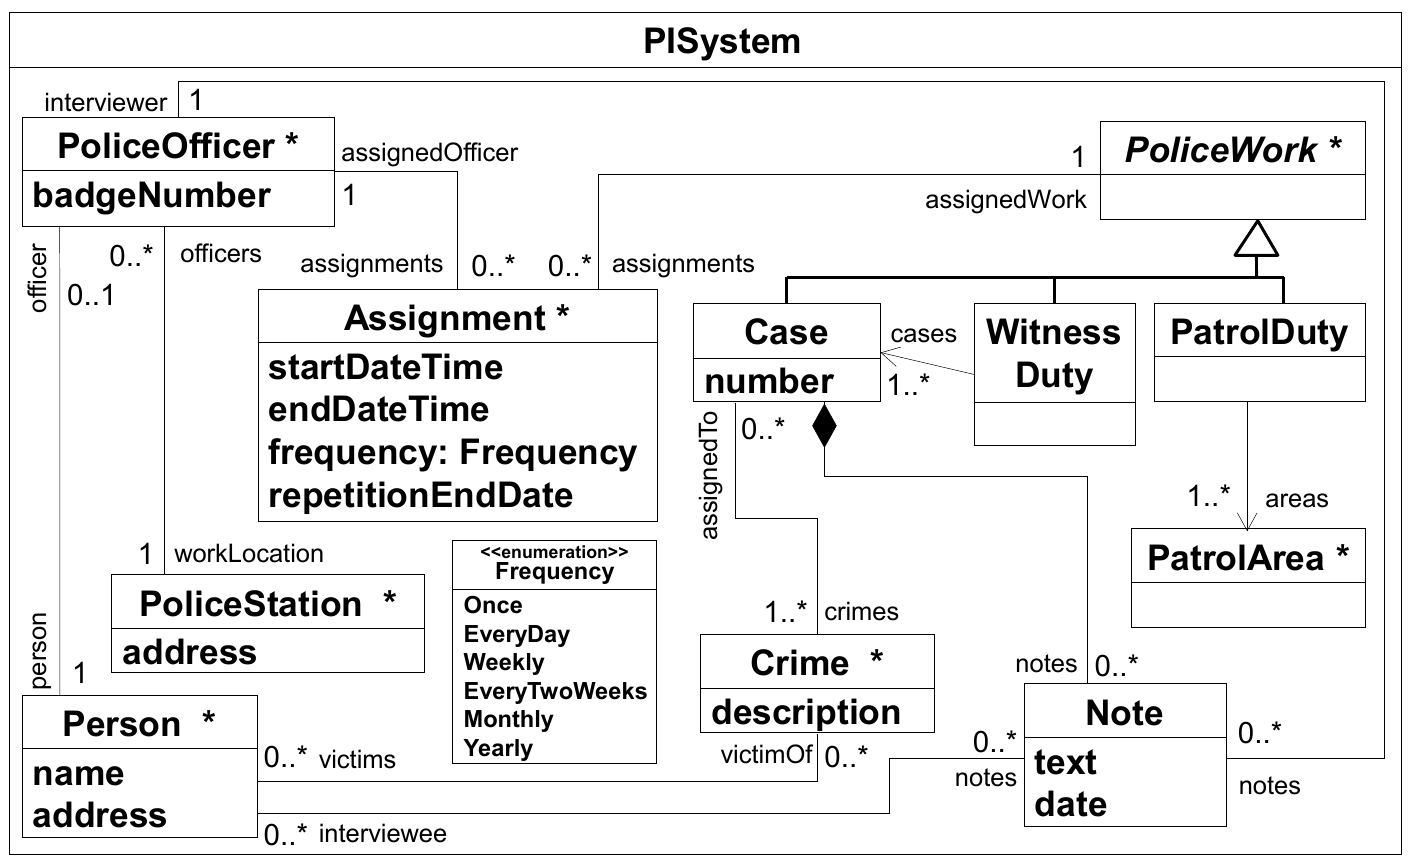
\includegraphics[width=0.6\textwidth]{images/PISystem.png}
\end{tabular} \medskip

\noindent Level 5: Resource response with List multiple-choice quiz: \medskip

\begin{tabular}{|p{0.9\linewidth}}

Which of the following compositions should be added to complete the containment tree for the
following model.

\\
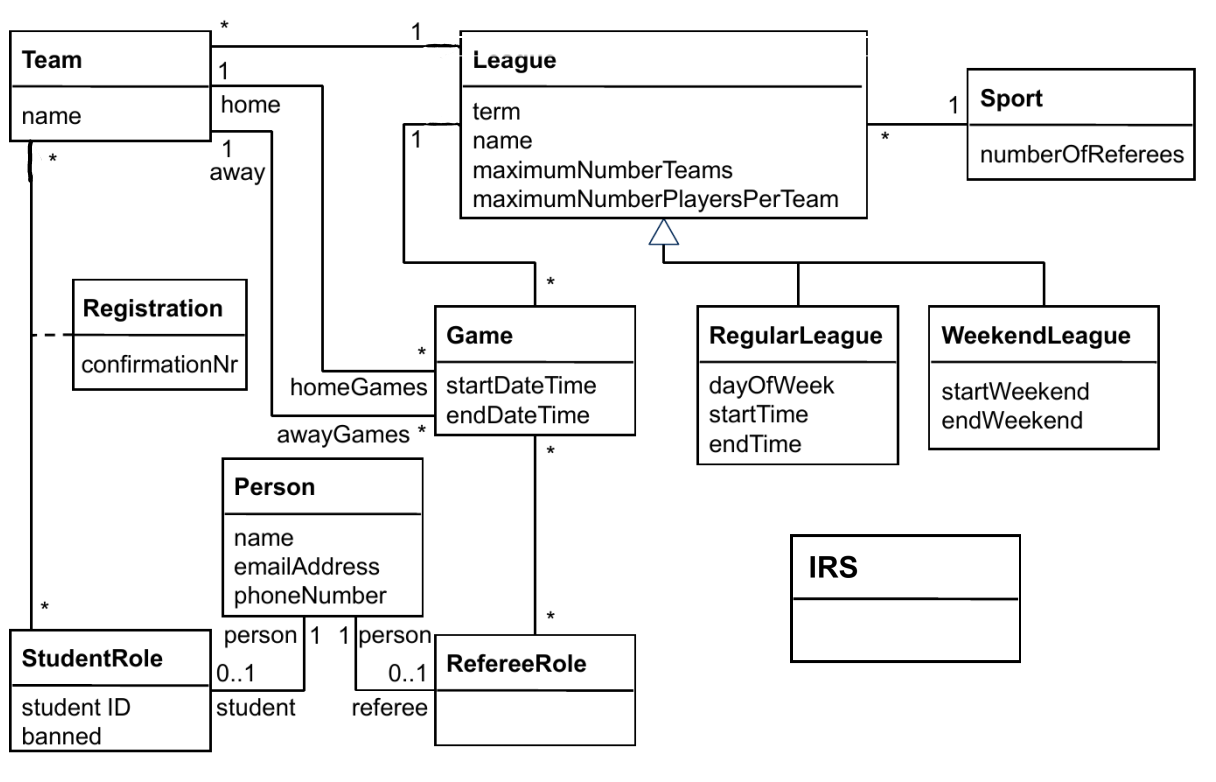
\includegraphics[width=0.6\textwidth]{images/IRS.png}

\begin{itemize}
    \item[$\boxtimes$] 1 IRS $<$@$>$- * StudentRole
    \item[$\boxtimes$] 1 IRS $<$@$>$- * Person
    \item[$\square$] 1 IRS $<$@$>$- * Game
    \item[$\boxtimes$] 1 IRS $<$@$>$- * League
    \item[$\square$] 1 IRS $<$@$>$- * RegularLeague
\end{itemize}

\end{tabular} \medskip

\noindent Level 6: Resource response with Reference: \medskip

\begin{tabular}{|p{0.9\linewidth}}
Please review the _Composition vs. Aggregation vs. Association_ section of 
the \textit{UML Class Diagram lecture slides} to 
better understand these relationships and where they are used.

\\
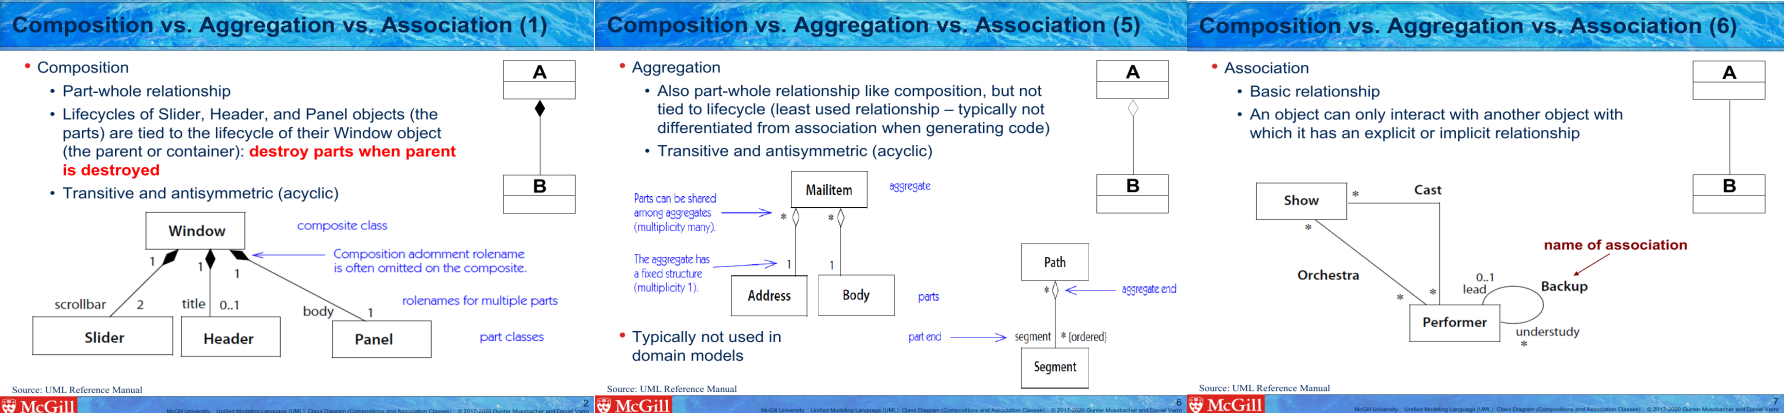
\includegraphics[width=0.9\textwidth]{images/composition_aggregation_association.png}
\end{tabular} \medskip


\subsection{Generalization mistakes}

\subsubsection{Missing generalization}

\noindent Level 1: Highlight solution (Class) \medskip

\noindent Level 2: Text response: \medskip

\begin{tabular}{|p{0.9\linewidth}}
What is the relationship between these classes?
\end{tabular} \medskip

\noindent Level 3: Parametrized response: \medskip

\begin{tabular}{|p{0.9\linewidth}}
A \verb|${subclass}| is a \verb|${superclass}|. How should we model this?
\end{tabular} \medskip

\noindent Level 4: Resource response with Fill-in-the-blanks quiz: \medskip

\begin{tabular}{|p{0.9\linewidth}}

Place the following classes in an inheritance hierarchy:

\begin{itemize}
    \item SportsCar isA \underline{Car}
    \item \underline{Wheel} isA VehiclePart
    \item Truck isA \underline{LandVehicle}
    \item AmphibiousVehicle isA \underline{Vehicle}
    \item \underline{LuxuryBus} isA BusVehicle
\end{itemize}

\end{tabular} \medskip

\noindent Level 5: Resource response with Reference: \medskip

\begin{tabular}{|p{0.9\linewidth}}
Please review the \textit{Generalization} part of the Class Diagram lecture.
\end{tabular} \medskip


\subsubsection{Extra generalization}

\noindent Level 1: Highlight solution (Class) \medskip

\noindent Level 2: Text response: \medskip

\begin{tabular}{|p{0.9\linewidth}}
Can you find a better way to express this relationship?
\end{tabular} \medskip

\noindent Level 3: Parametrized response: \medskip

\begin{tabular}{|p{0.9\linewidth}}
When creating a generalization between \verb|${wrongSubclass}| and \verb|${wrongSuperclass}|, make sure to follow the \textit{checks for proper generalization}.
\end{tabular} \medskip

\noindent Level 4: Resource response with Fill-in-the-blanks quiz: \medskip

\begin{tabular}{|p{0.9\linewidth}}

Place the following classes in an inheritance hierarchy:

\begin{itemize}
    \item SportsCar isA \underline{Car}
    \item \underline{Wheel} isA VehiclePart
    \item Truck isA \underline{LandVehicle}
    \item AmphibiousVehicle isA \underline{Vehicle}
    \item \underline{LuxuryBus} isA BusVehicle
\end{itemize}

\end{tabular} \medskip

\noindent Level 5: Resource response with Fill-in-the-blanks quiz: \medskip

\begin{tabular}{|p{0.9\linewidth}}

Please review the \textit{checks for proper generalization} lecture material
and complete the following:

The five checks for generalization are:

\begin{itemize}
    \item Obeys the \underline{isA rule}.
    \item Subclass must retain its \underline{distinctiveness}.
    \item All \underline{inherited features} must make sense in each subclass.
    \item Subclass differs from superclass and other subclasses in \underline{behavior} or \underline{structure}.
    \item Subclass must not be \underline{an instance}.
\end{itemize}

\end{tabular} \medskip

\noindent Level 6: Resource response with Reference: \medskip

\begin{tabular}{|p{0.9\linewidth}}
Please review the \textit{Generalization} part of the Class Diagram lecture.
\end{tabular} \medskip


\subsubsection{Generalization does not follow isA rule}

\noindent Level 1: Highlight solution  \medskip

\noindent Level 2: Text response: \medskip

\begin{tabular}{|p{0.9\linewidth}}
Can you find a better way to express this relationship?
\end{tabular} \medskip

\noindent Level 3: Parametrized response: \medskip

\begin{tabular}{|p{0.9\linewidth}}
When creating a generalization between \verb|${wrongSubclass}| and \verb|${wrongSuperclass}|, make sure to follow the \textit{checks for proper generalization}.
\end{tabular} \medskip

\noindent Level 4: Resource response with Fill-in-the-blanks quiz: \medskip

\begin{tabular}{|p{0.9\linewidth}}

Place the following classes in an inheritance hierarchy:

\begin{itemize}
    \item SportsCar isA \underline{Car}
    \item \underline{Wheel} isA VehiclePart
    \item Truck isA \underline{LandVehicle}
    \item AmphibiousVehicle isA \underline{Vehicle}
    \item \underline{LuxuryBus} isA BusVehicle
\end{itemize}

\end{tabular} \medskip

\noindent Level 5: Resource response with Fill-in-the-blanks quiz: \medskip

\begin{tabular}{|p{0.9\linewidth}}

Please review the \textit{checks for proper generalization} lecture material
and complete the following:

The five checks for generalization are:

\begin{itemize}
    \item Obeys the \underline{isA rule}.
    \item Subclass must retain its \underline{distinctiveness}.
    \item All \underline{inherited features} must make sense in each subclass.
    \item Subclass differs from superclass and other subclasses in \underline{behavior} or \underline{structure}.
    \item Subclass must not be \underline{an instance}.
\end{itemize}

\end{tabular} \medskip

\noindent Level 6: Resource response with Reference: \medskip

\begin{tabular}{|p{0.9\linewidth}}
Please review the \textit{Generalization} part of the Class Diagram lecture.
\end{tabular} \medskip


\subsubsection{Subclass not distinct across lifetime}

\noindent Level 1: Highlight solution  \medskip

\noindent Level 2: Text response: \medskip

\begin{tabular}{|p{0.9\linewidth}}
Can you find a better way to model this concept?
\end{tabular} \medskip

\noindent Level 3: Parametrized response: \medskip

\begin{tabular}{|p{0.9\linewidth}}
Is it possible for an instance of \verb|${nondistinctSubclass}| to turn into an instance of another subclass over its lifetime?
\end{tabular} \medskip

\noindent Level 4: Resource response with List multiple-choice quiz: \medskip

\begin{tabular}{|p{0.9\linewidth}}

Which classes are not subclasses of Account?

\begin{itemize}
    \item[$\square$] SavingsAccount
    \item[$\boxtimes$] OverdrawnAccount
    \item[$\square$] CheckingAccount
    \item[$\square$] MortgageAccount
    \item[$\boxtimes$] ClosedAccount
\end{itemize}

\end{tabular} \medskip

\noindent Level 5: Resource response with Reference: \medskip

\begin{tabular}{|p{0.9\linewidth}}
Please review the \textit{Generalization} part of the Class Diagram lecture.
\end{tabular} \medskip


\subsubsection{Inherited feature does not make sense for subclass}

\noindent Level 1: Highlight solution  \medskip

\noindent Level 2: Text response: \medskip

\begin{tabular}{|p{0.9\linewidth}}
Does this belong here?
\end{tabular} \medskip

\noindent Level 3: Parametrized response: \medskip

\begin{tabular}{|p{0.9\linewidth}}
The \verb|${featureName}| feature of the \verb|${superclass}| class does not make sense for its \verb|${subclass}| subclass.
\end{tabular} \medskip

\noindent Level 4: Resource response with Fill-in-the-blanks quiz: \medskip

\begin{tabular}{|p{0.9\linewidth}}

Please review the \textit{checks for proper generalization} lecture material
and complete the following:

The five checks for generalization are:

\begin{itemize}
    \item Obeys the \underline{isA rule}.
    \item Subclass must retain its \underline{distinctiveness}.
    \item All \underline{inherited features} must make sense in each subclass.
    \item Subclass differs from superclass and other subclasses in \underline{behavior} or \underline{structure}.
    \item Subclass must not be \underline{an instance}.
\end{itemize}

\end{tabular} \medskip

\noindent Level 5: Resource response with Reference: \medskip

\begin{tabular}{|p{0.9\linewidth}}
Please review the \textit{Generalization} part of the Class Diagram lecture.
\end{tabular} \medskip


\subsubsection{Subclass is an instance of superclass}

\noindent Level 1: Highlight solution  \medskip

\noindent Level 2: Text response: \medskip

\begin{tabular}{|p{0.9\linewidth}}
Can you find a better way to express this relationship?
\end{tabular} \medskip

\noindent Level 3: Text response: \medskip

\begin{tabular}{|p{0.9\linewidth}}
Remember the definition of the **'instance' rule**.[ Instances should not be modeled as subclasses].
\end{tabular} \medskip

\noindent Level 4: Resource response with Example: \medskip

\begin{tabular}{|p{0.9\linewidth}}
A CheckingAccount isA Account, but account1234 is **not** an Account according to the 'instance' rule.
\end{tabular} \medskip

\noindent Level 5: Resource response with Fill-in-the-blanks quiz: \medskip

\begin{tabular}{|p{0.9\linewidth}}

Please review the \textit{checks for proper generalization} lecture material
and complete the following:

The five checks for generalization are:

\begin{itemize}
    \item Obeys the \underline{isA rule}.
    \item Subclass must retain its \underline{distinctiveness}.
    \item All \underline{inherited features} must make sense in each subclass.
    \item Subclass differs from superclass and other subclasses in \underline{behavior} or \underline{structure}.
    \item Subclass must not be \underline{an instance}.
\end{itemize}

\end{tabular} \medskip

\noindent Level 6: Resource response with Reference: \medskip

\begin{tabular}{|p{0.9\linewidth}}
Please review the \textit{Generalization} part of the Class Diagram lecture.
\end{tabular} \medskip


\subsubsection{Non-differentiated subclass}

\noindent Level 1: Highlight solution (Class) \medskip

\noindent Level 2: Text response: \medskip

\begin{tabular}{|p{0.9\linewidth}}
Is it really necessary to model this as a subclass?
\end{tabular} \medskip

\noindent Level 3: Parametrized response: \medskip

\begin{tabular}{|p{0.9\linewidth}}
\verb|${stud_cls}| needs to be different from its superclass, and any sibling subclasses, in terms of behavior or structure.
\end{tabular} \medskip

\noindent Level 4: Resource response with Fill-in-the-blanks quiz: \medskip

\begin{tabular}{|p{0.9\linewidth}}

Please review the \textit{checks for proper generalization} lecture material
and complete the following:

The five checks for generalization are:

\begin{itemize}
    \item Obeys the \underline{isA rule}.
    \item Subclass must retain its \underline{distinctiveness}.
    \item All \underline{inherited features} must make sense in each subclass.
    \item Subclass differs from superclass and other subclasses in \underline{behavior} or \underline{structure}.
    \item Subclass must not be \underline{an instance}.
\end{itemize}

\end{tabular} \medskip

\noindent Level 5: Resource response with Reference: \medskip

\begin{tabular}{|p{0.9\linewidth}}
Please review the \textit{Generalization} part of the Class Diagram lecture.
\end{tabular} \medskip


\subsubsection{Wrong generalization direction}

\noindent Level 1: Highlight solution (Class) \medskip

\noindent Level 2: Text response: \medskip

\begin{tabular}{|p{0.9\linewidth}}
Can you double check this relationship?
\end{tabular} \medskip

\noindent Level 3: Parametrized response: \medskip

\begin{tabular}{|p{0.9\linewidth}}
Is \verb|${superclass}| really a \verb|${subclass}|?[ It should be the other way around.]
\end{tabular} \medskip

\noindent Level 4: Resource response with Fill-in-the-blanks quiz: \medskip

\begin{tabular}{|p{0.9\linewidth}}

Place the following classes in an inheritance hierarchy:

\begin{itemize}
    \item SportsCar isA \underline{Car}
    \item \underline{Wheel} isA VehiclePart
    \item Truck isA \underline{LandVehicle}
    \item AmphibiousVehicle isA \underline{Vehicle}
    \item \underline{LuxuryBus} isA BusVehicle
\end{itemize}

\end{tabular} \medskip

\noindent Level 5: Resource response with Fill-in-the-blanks quiz: \medskip

\begin{tabular}{|p{0.9\linewidth}}

Please review the \textit{checks for proper generalization} lecture material
and complete the following:

The five checks for generalization are:

\begin{itemize}
    \item Obeys the \underline{isA rule}.
    \item Subclass must retain its \underline{distinctiveness}.
    \item All \underline{inherited features} must make sense in each subclass.
    \item Subclass differs from superclass and other subclasses in \underline{behavior} or \underline{structure}.
    \item Subclass must not be \underline{an instance}.
\end{itemize}

\end{tabular} \medskip

\noindent Level 6: Resource response with Reference: \medskip

\begin{tabular}{|p{0.9\linewidth}}
Please review the \textit{Generalization} part of the Class Diagram lecture.
\end{tabular} \medskip


\subsubsection{Wrong superclass}

\noindent Level 1: Highlight solution (Class) \medskip

\noindent Level 2: Text response: \medskip

\begin{tabular}{|p{0.9\linewidth}}
Can you double check this relationship?
\end{tabular} \medskip

\noindent Level 3: Parametrized response: \medskip

\begin{tabular}{|p{0.9\linewidth}}
Can you (find$|$create) a (better$|$different) superclass for \verb|${subclass}|?[ Look at the problem description closely].
\end{tabular} \medskip

\noindent Level 4: Highlight specific problem statement elements \medskip

\noindent Level 5: Parametrized response: \medskip

\begin{tabular}{|p{0.9\linewidth}}
What is the inheritance hierarchy between \verb|${hierarchy.classes}|?
\end{tabular} \medskip

\noindent Level 6: Resource response with Fill-in-the-blanks quiz: \medskip

\begin{tabular}{|p{0.9\linewidth}}

Place the following classes in an inheritance hierarchy:

\begin{itemize}
    \item SportsCar isA \underline{Car}
    \item \underline{Wheel} isA VehiclePart
    \item Truck isA \underline{LandVehicle}
    \item AmphibiousVehicle isA \underline{Vehicle}
    \item \underline{LuxuryBus} isA BusVehicle
\end{itemize}

\end{tabular} \medskip

\noindent Level 7: Resource response with Reference: \medskip

\begin{tabular}{|p{0.9\linewidth}}
Please review the \textit{Generalization} part of the Class Diagram lecture.
\end{tabular} \medskip




\section{Design pattern mistakes}

\subsection{Player-Role Pattern mistakes}

\subsubsection{Missing Player-Role pattern}

\noindent Level 1: Highlight solution  \medskip

\noindent Level 2: Text response: \medskip

\begin{tabular}{|p{0.9\linewidth}}
Think carefully about how to model the relationships between these concepts.
\end{tabular} \medskip

\noindent Level 3: Parametrized response: \medskip

\begin{tabular}{|p{0.9\linewidth}}
The concepts of \verb|${instructorPlayer}| and \verb|${instructorRole}| and the relationship between them should be modeled with one of the forms of the Player-Role pattern.
\end{tabular} \medskip

\noindent Level 4: Resource response with Quiz: \medskip


\begin{tabular}{lcccc}
\hline
\textbf{Solution} &
  \textbf{\begin{tabular}[c]{@{}c@{}}Roles\\ have\\ different\\ features\end{tabular}} &
  \textbf{\begin{tabular}[c]{@{}c@{}}Only one\\ role at\\ a time\end{tabular}} &
  \textbf{\begin{tabular}[c]{@{}c@{}}Different\\ roles\\ over time\end{tabular}} &
  \textbf{\begin{tabular}[c]{@{}c@{}}More than\\ one role\\ at the\\ same time\end{tabular}} \\ \hline
Enumeration         & $\square$   & $\boxtimes$ & $\boxtimes$ & $\square$   \\
Subclasses          & $\boxtimes$ & $\boxtimes$ & $\square$   & $\square$   \\
Associations        & $\square$   & $\boxtimes$ & $\boxtimes$ & $\boxtimes$ \\
Player-Role Pattern & $\boxtimes$ & $\boxtimes$ & $\boxtimes$ & $\boxtimes$ \\ \hline
\end{tabular} \bigskip


\noindent Level 5: Resource response with Reference: \medskip

\begin{tabular}{|p{0.9\linewidth}}
The Player-Role Pattern can be used to capture the fact that an object may play different roles
in different contexts.

\\
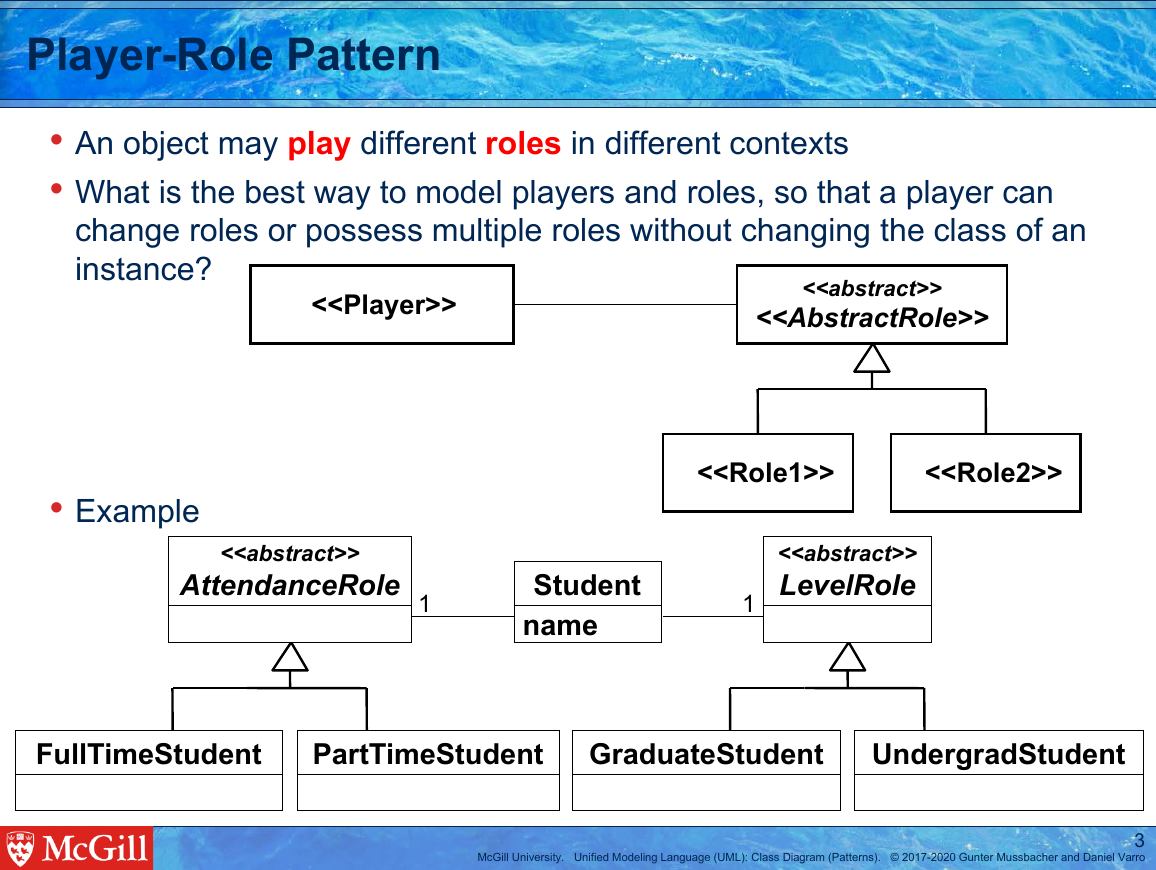
\includegraphics[width=0.6\textwidth]{images/player_role.png}
\end{tabular} \medskip


\subsubsection{Incomplete Player-Role pattern}

\noindent Level 1: Highlight solution (Class) \medskip

\noindent Level 2: Text response: \medskip

\begin{tabular}{|p{0.9\linewidth}}
Think carefully about how to model the relationships between these concepts.
\end{tabular} \medskip

\noindent Level 3: Parametrized response: \medskip

\begin{tabular}{|p{0.9\linewidth}}
The concepts of \verb|${instructorPlayer}| and \verb|${instructorRole}| and the relationship between them should be modeled with one of the forms of the Player-Role pattern.
\end{tabular} \medskip

\noindent Level 4: Resource response with Quiz: \medskip


\begin{tabular}{lcccc}
\hline
\textbf{Solution} &
  \textbf{\begin{tabular}[c]{@{}c@{}}Roles\\ have\\ different\\ features\end{tabular}} &
  \textbf{\begin{tabular}[c]{@{}c@{}}Only one\\ role at\\ a time\end{tabular}} &
  \textbf{\begin{tabular}[c]{@{}c@{}}Different\\ roles\\ over time\end{tabular}} &
  \textbf{\begin{tabular}[c]{@{}c@{}}More than\\ one role\\ at the\\ same time\end{tabular}} \\ \hline
Enumeration         & $\square$   & $\boxtimes$ & $\boxtimes$ & $\square$   \\
Subclasses          & $\boxtimes$ & $\boxtimes$ & $\square$   & $\square$   \\
Associations        & $\square$   & $\boxtimes$ & $\boxtimes$ & $\boxtimes$ \\
Player-Role Pattern & $\boxtimes$ & $\boxtimes$ & $\boxtimes$ & $\boxtimes$ \\ \hline
\end{tabular} \bigskip


\noindent Level 5: Resource response with Reference: \medskip

\begin{tabular}{|p{0.9\linewidth}}
The Player-Role Pattern can be used to capture the fact that an object may play different roles
in different contexts.

\\
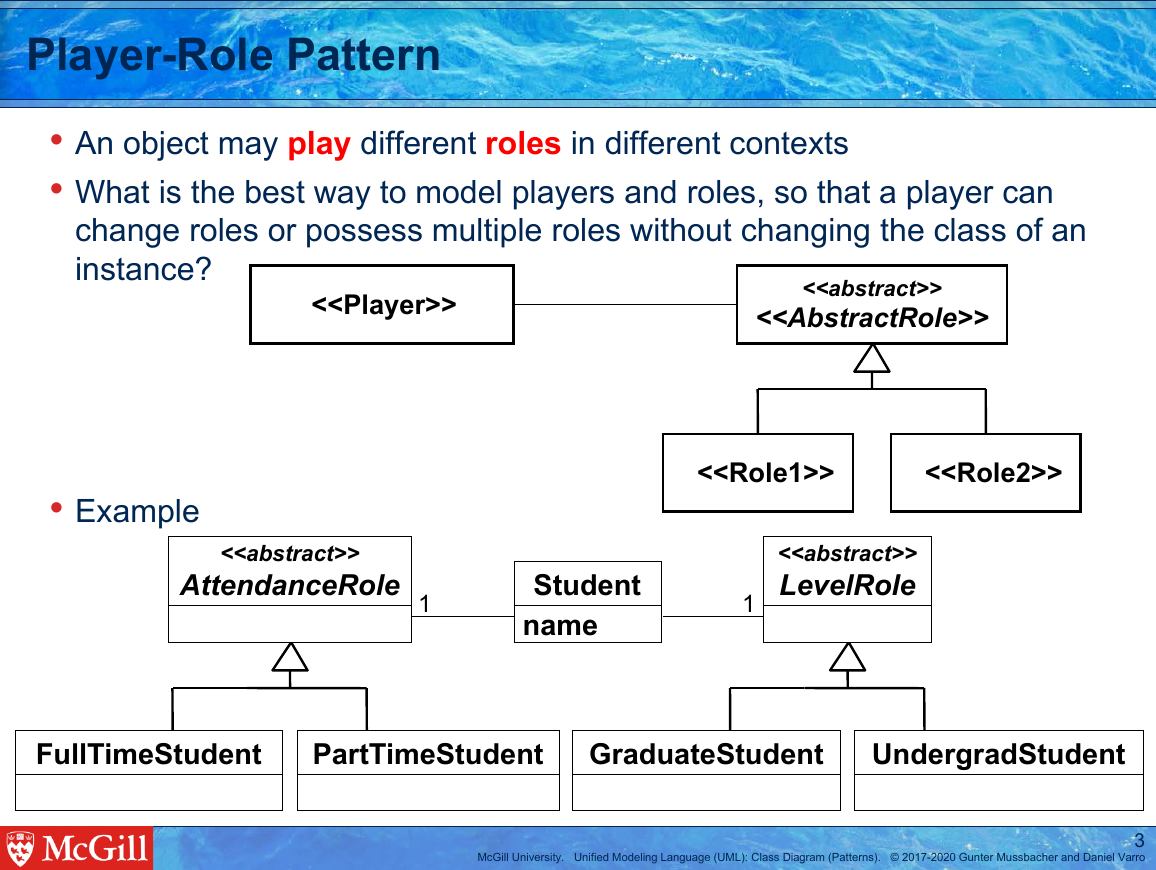
\includegraphics[width=0.6\textwidth]{images/player_role.png}
\end{tabular} \medskip


\subsubsection{Subclass should be full Player-Role pattern}

\noindent Level 1: Highlight solution (Class) \medskip

\noindent Level 2: Text response: \medskip

\begin{tabular}{|p{0.9\linewidth}}
Think carefully about how to model the relationships between these concepts.
\end{tabular} \medskip

\noindent Level 3: Parametrized response: \medskip

\begin{tabular}{|p{0.9\linewidth}}
[Nice try, but] a \verb|${firstSubclass}| can also play the role of one of the other subclasses.
\end{tabular} \medskip

\noindent Level 4: Resource response with Quiz: \medskip


\begin{tabular}{lcccc}
\hline
\textbf{Solution} &
  \textbf{\begin{tabular}[c]{@{}c@{}}Roles\\ have\\ different\\ features\end{tabular}} &
  \textbf{\begin{tabular}[c]{@{}c@{}}Only one\\ role at\\ a time\end{tabular}} &
  \textbf{\begin{tabular}[c]{@{}c@{}}Different\\ roles\\ over time\end{tabular}} &
  \textbf{\begin{tabular}[c]{@{}c@{}}More than\\ one role\\ at the\\ same time\end{tabular}} \\ \hline
Enumeration         & $\square$   & $\boxtimes$ & $\boxtimes$ & $\square$   \\
Subclasses          & $\boxtimes$ & $\boxtimes$ & $\square$   & $\square$   \\
Associations        & $\square$   & $\boxtimes$ & $\boxtimes$ & $\boxtimes$ \\
Player-Role Pattern & $\boxtimes$ & $\boxtimes$ & $\boxtimes$ & $\boxtimes$ \\ \hline
\end{tabular} \bigskip


\noindent Level 5: Resource response with Reference: \medskip

\begin{tabular}{|p{0.9\linewidth}}
The Player-Role Pattern can be used to capture the fact that an object may play different roles
in different contexts.

\\
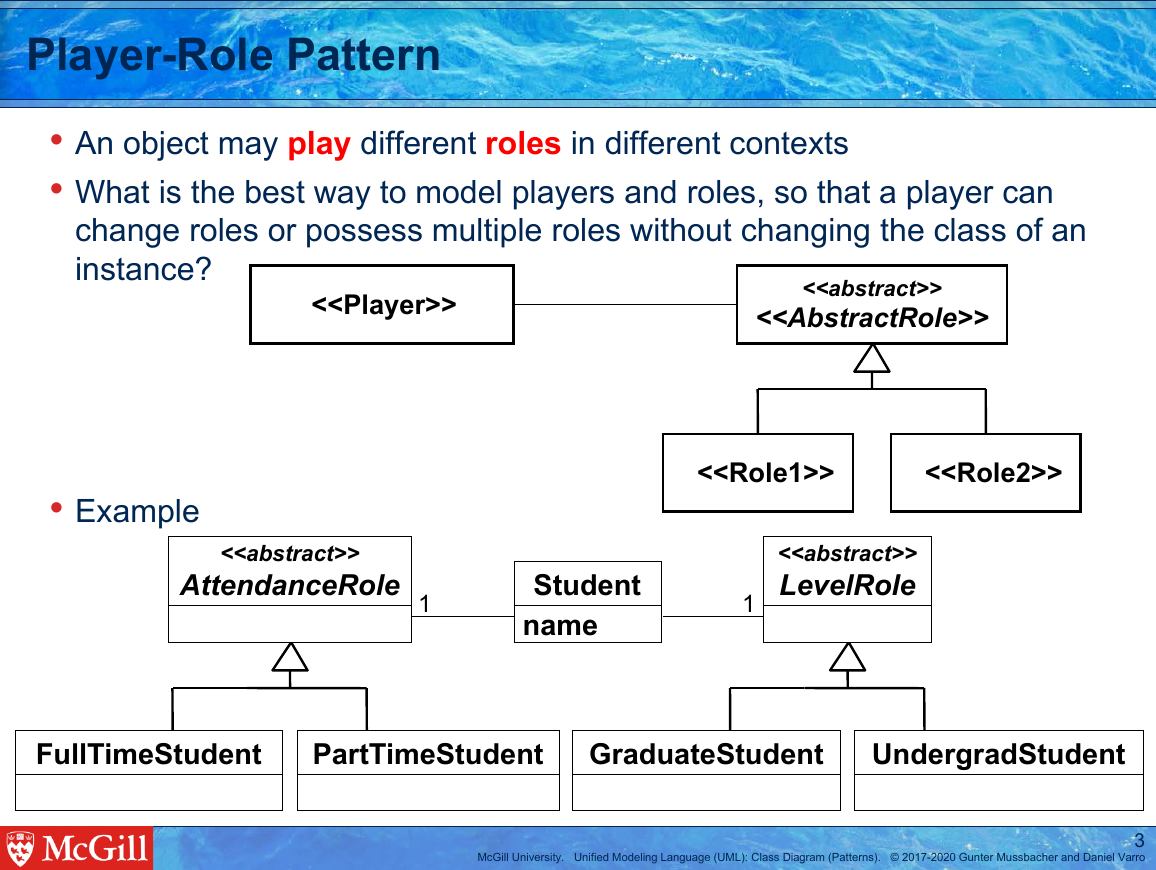
\includegraphics[width=0.6\textwidth]{images/player_role.png}
\end{tabular} \medskip


\subsubsection{Subclass should be association Player-Role pattern}

\noindent Level 1: Highlight solution (Relationship) \medskip

\noindent Level 2: Text response: \medskip

\begin{tabular}{|p{0.9\linewidth}}
Think carefully about how to model the relationships between these concepts.
\end{tabular} \medskip

\noindent Level 3: Parametrized response: \medskip

\begin{tabular}{|p{0.9\linewidth}}
[Nice try, but] a \verb|${firstSubclass}| can also play the role of one of the other subclasses and different features do not need to be captured for the subclasses.
\end{tabular} \medskip

\noindent Level 4: Resource response with Quiz: \medskip


\begin{tabular}{lcccc}
\hline
\textbf{Solution} &
  \textbf{\begin{tabular}[c]{@{}c@{}}Roles\\ have\\ different\\ features\end{tabular}} &
  \textbf{\begin{tabular}[c]{@{}c@{}}Only one\\ role at\\ a time\end{tabular}} &
  \textbf{\begin{tabular}[c]{@{}c@{}}Different\\ roles\\ over time\end{tabular}} &
  \textbf{\begin{tabular}[c]{@{}c@{}}More than\\ one role\\ at the\\ same time\end{tabular}} \\ \hline
Enumeration         & $\square$   & $\boxtimes$ & $\boxtimes$ & $\square$   \\
Subclasses          & $\boxtimes$ & $\boxtimes$ & $\square$   & $\square$   \\
Associations        & $\square$   & $\boxtimes$ & $\boxtimes$ & $\boxtimes$ \\
Player-Role Pattern & $\boxtimes$ & $\boxtimes$ & $\boxtimes$ & $\boxtimes$ \\ \hline
\end{tabular} \bigskip


\noindent Level 5: Resource response with Reference: \medskip

\begin{tabular}{|p{0.9\linewidth}}
The Player-Role Pattern can be used to capture the fact that an object may play different roles
in different contexts.

\\
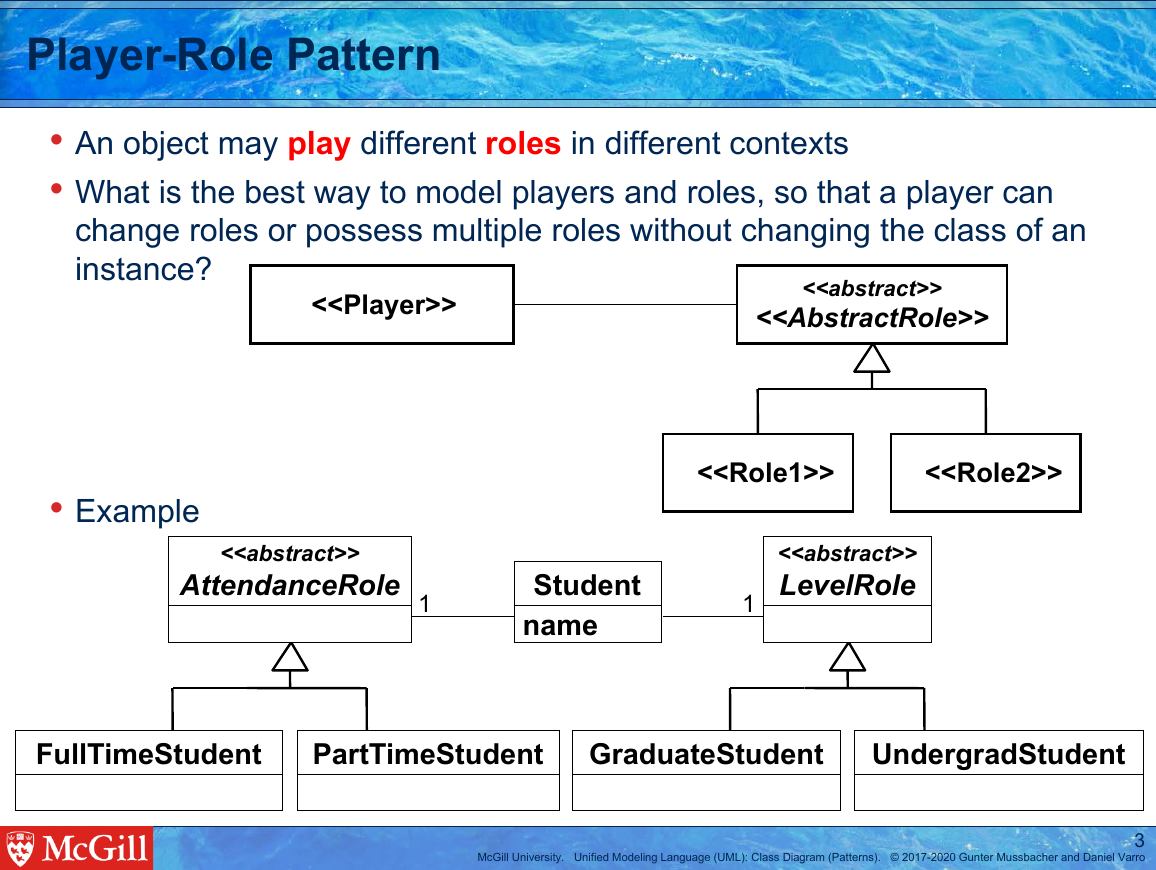
\includegraphics[width=0.6\textwidth]{images/player_role.png}
\end{tabular} \medskip


\subsubsection{Subclass should be enumeration Player-Role pattern}

\noindent Level 1: Highlight solution (Attribute) \medskip

\noindent Level 2: Text response: \medskip

\begin{tabular}{|p{0.9\linewidth}}
Think carefully about how to model the relationships between these concepts.
\end{tabular} \medskip

\noindent Level 3: Parametrized response: \medskip

\begin{tabular}{|p{0.9\linewidth}}
[Nice try, but] a \verb|${firstSubclass}| does not need to play the role of one of the other subclasses and different features do not need to be captured for the subclasses.
\end{tabular} \medskip

\noindent Level 4: Resource response with Quiz: \medskip


\begin{tabular}{lcccc}
\hline
\textbf{Solution} &
  \textbf{\begin{tabular}[c]{@{}c@{}}Roles\\ have\\ different\\ features\end{tabular}} &
  \textbf{\begin{tabular}[c]{@{}c@{}}Only one\\ role at\\ a time\end{tabular}} &
  \textbf{\begin{tabular}[c]{@{}c@{}}Different\\ roles\\ over time\end{tabular}} &
  \textbf{\begin{tabular}[c]{@{}c@{}}More than\\ one role\\ at the\\ same time\end{tabular}} \\ \hline
Enumeration         & $\square$   & $\boxtimes$ & $\boxtimes$ & $\square$   \\
Subclasses          & $\boxtimes$ & $\boxtimes$ & $\square$   & $\square$   \\
Associations        & $\square$   & $\boxtimes$ & $\boxtimes$ & $\boxtimes$ \\
Player-Role Pattern & $\boxtimes$ & $\boxtimes$ & $\boxtimes$ & $\boxtimes$ \\ \hline
\end{tabular} \bigskip


\noindent Level 5: Resource response with Reference: \medskip

\begin{tabular}{|p{0.9\linewidth}}
The Player-Role Pattern can be used to capture the fact that an object may play different roles
in different contexts.

\\
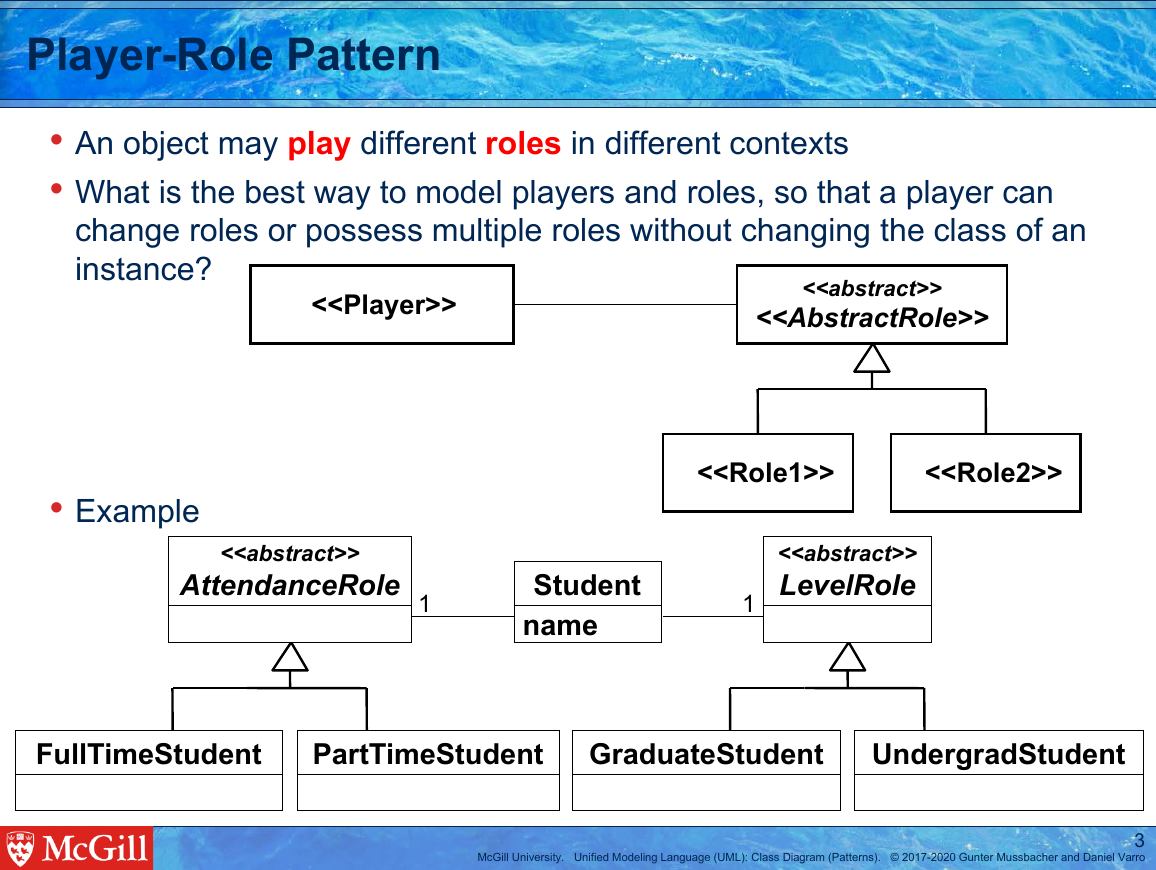
\includegraphics[width=0.6\textwidth]{images/player_role.png}
\end{tabular} \medskip


\subsubsection{Association should be full Player-Role pattern}

\noindent Level 1: Highlight solution (Relationship) \medskip

\noindent Level 2: Text response: \medskip

\begin{tabular}{|p{0.9\linewidth}}
Think carefully about how to model the relationships between these concepts.
\end{tabular} \medskip

\noindent Level 3: Parametrized response: \medskip

\begin{tabular}{|p{0.9\linewidth}}
A \verb|${firstRole}| has different features from a \verb|${secondRole}|.
\end{tabular} \medskip

\noindent Level 4: Resource response with Quiz: \medskip


\begin{tabular}{lcccc}
\hline
\textbf{Solution} &
  \textbf{\begin{tabular}[c]{@{}c@{}}Roles\\ have\\ different\\ features\end{tabular}} &
  \textbf{\begin{tabular}[c]{@{}c@{}}Only one\\ role at\\ a time\end{tabular}} &
  \textbf{\begin{tabular}[c]{@{}c@{}}Different\\ roles\\ over time\end{tabular}} &
  \textbf{\begin{tabular}[c]{@{}c@{}}More than\\ one role\\ at the\\ same time\end{tabular}} \\ \hline
Enumeration         & $\square$   & $\boxtimes$ & $\boxtimes$ & $\square$   \\
Subclasses          & $\boxtimes$ & $\boxtimes$ & $\square$   & $\square$   \\
Associations        & $\square$   & $\boxtimes$ & $\boxtimes$ & $\boxtimes$ \\
Player-Role Pattern & $\boxtimes$ & $\boxtimes$ & $\boxtimes$ & $\boxtimes$ \\ \hline
\end{tabular} \bigskip


\noindent Level 5: Resource response with Reference: \medskip

\begin{tabular}{|p{0.9\linewidth}}
The Player-Role Pattern can be used to capture the fact that an object may play different roles
in different contexts.

\\
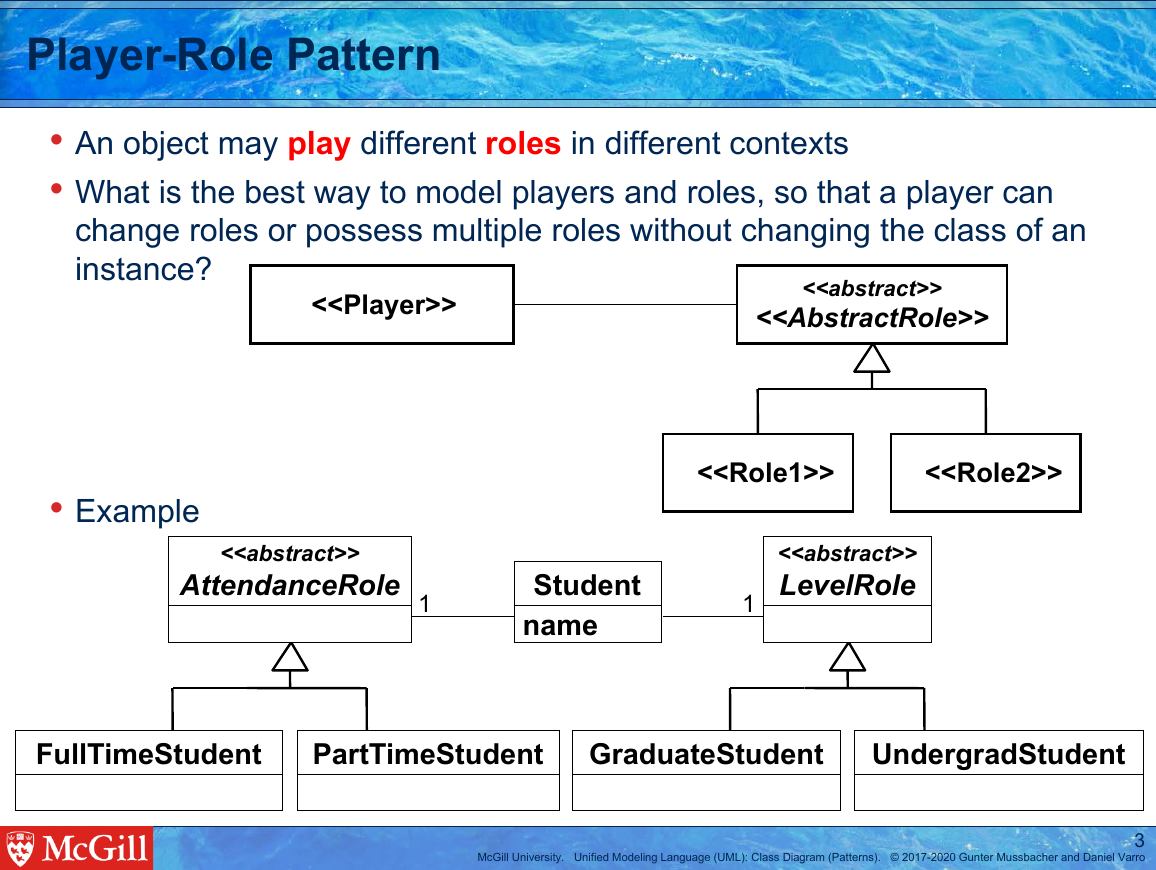
\includegraphics[width=0.6\textwidth]{images/player_role.png}
\end{tabular} \medskip


\subsubsection{Association should be subclass Player-Role pattern}

\noindent Level 1: Highlight solution (Relationship) \medskip

\noindent Level 2: Text response: \medskip

\begin{tabular}{|p{0.9\linewidth}}
Think carefully about how to model the relationships between these concepts.
\end{tabular} \medskip

\noindent Level 3: Parametrized response: \medskip

\begin{tabular}{|p{0.9\linewidth}}
A \verb|${firstRole}| has different features from a \verb|${secondRole}| and \verb|${role}| does not change its role over its lifetime.
\end{tabular} \medskip

\noindent Level 4: Resource response with Quiz: \medskip


\begin{tabular}{lcccc}
\hline
\textbf{Solution} &
  \textbf{\begin{tabular}[c]{@{}c@{}}Roles\\ have\\ different\\ features\end{tabular}} &
  \textbf{\begin{tabular}[c]{@{}c@{}}Only one\\ role at\\ a time\end{tabular}} &
  \textbf{\begin{tabular}[c]{@{}c@{}}Different\\ roles\\ over time\end{tabular}} &
  \textbf{\begin{tabular}[c]{@{}c@{}}More than\\ one role\\ at the\\ same time\end{tabular}} \\ \hline
Enumeration         & $\square$   & $\boxtimes$ & $\boxtimes$ & $\square$   \\
Subclasses          & $\boxtimes$ & $\boxtimes$ & $\square$   & $\square$   \\
Associations        & $\square$   & $\boxtimes$ & $\boxtimes$ & $\boxtimes$ \\
Player-Role Pattern & $\boxtimes$ & $\boxtimes$ & $\boxtimes$ & $\boxtimes$ \\ \hline
\end{tabular} \bigskip


\noindent Level 5: Resource response with Reference: \medskip

\begin{tabular}{|p{0.9\linewidth}}
The Player-Role Pattern can be used to capture the fact that an object may play different roles
in different contexts.

\\
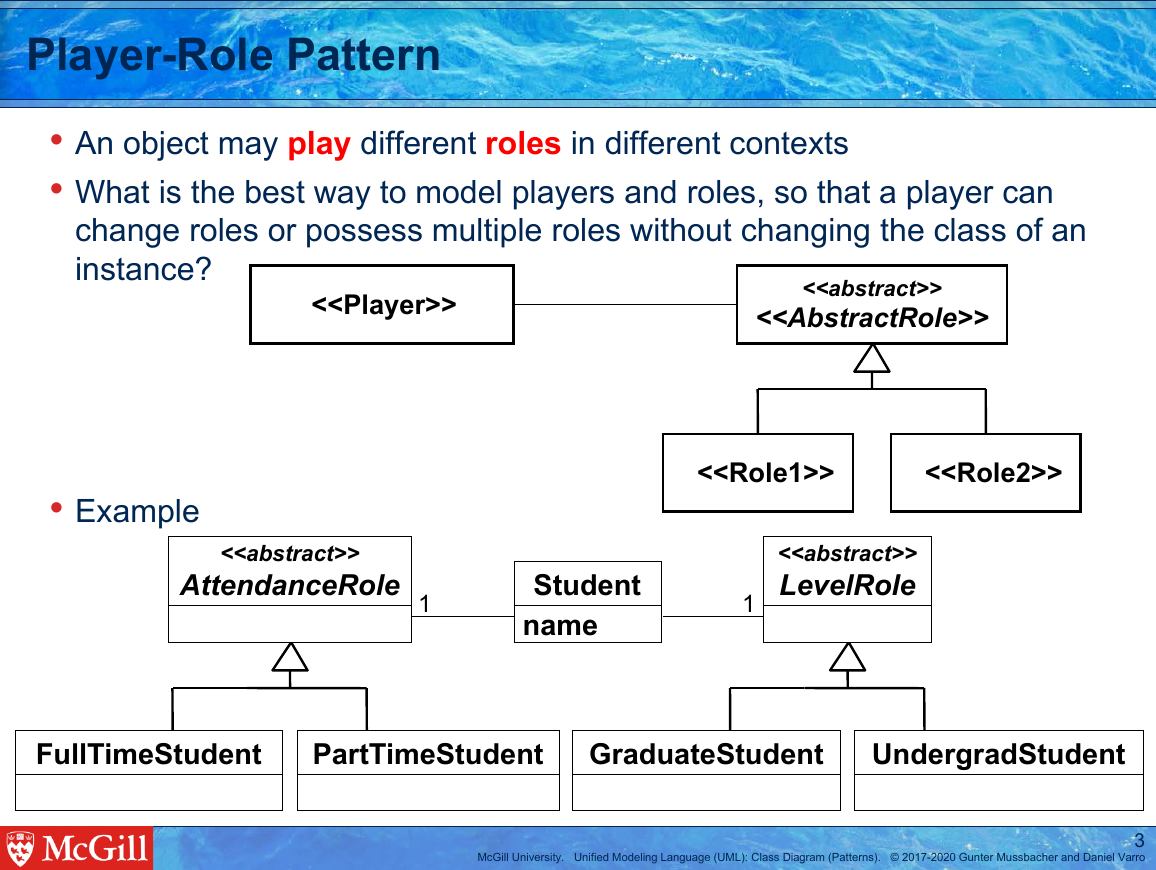
\includegraphics[width=0.6\textwidth]{images/player_role.png}
\end{tabular} \medskip


\subsubsection{Association should be enumeration Player-Role pattern}

\noindent Level 1: Highlight solution (Relationship) \medskip

\noindent Level 2: Text response: \medskip

\begin{tabular}{|p{0.9\linewidth}}
Think carefully about how to model the relationships between these concepts.
\end{tabular} \medskip

\noindent Level 3: Parametrized response: \medskip

\begin{tabular}{|p{0.9\linewidth}}
Will the roles of \verb|${firstRole}| and \verb|${secondRole}| ever be occupied at the same time?
\end{tabular} \medskip

\noindent Level 4: Resource response with Quiz: \medskip


\begin{tabular}{lcccc}
\hline
\textbf{Solution} &
  \textbf{\begin{tabular}[c]{@{}c@{}}Roles\\ have\\ different\\ features\end{tabular}} &
  \textbf{\begin{tabular}[c]{@{}c@{}}Only one\\ role at\\ a time\end{tabular}} &
  \textbf{\begin{tabular}[c]{@{}c@{}}Different\\ roles\\ over time\end{tabular}} &
  \textbf{\begin{tabular}[c]{@{}c@{}}More than\\ one role\\ at the\\ same time\end{tabular}} \\ \hline
Enumeration         & $\square$   & $\boxtimes$ & $\boxtimes$ & $\square$   \\
Subclasses          & $\boxtimes$ & $\boxtimes$ & $\square$   & $\square$   \\
Associations        & $\square$   & $\boxtimes$ & $\boxtimes$ & $\boxtimes$ \\
Player-Role Pattern & $\boxtimes$ & $\boxtimes$ & $\boxtimes$ & $\boxtimes$ \\ \hline
\end{tabular} \bigskip


\noindent Level 5: Resource response with Reference: \medskip

\begin{tabular}{|p{0.9\linewidth}}
The Player-Role Pattern can be used to capture the fact that an object may play different roles
in different contexts.

\\
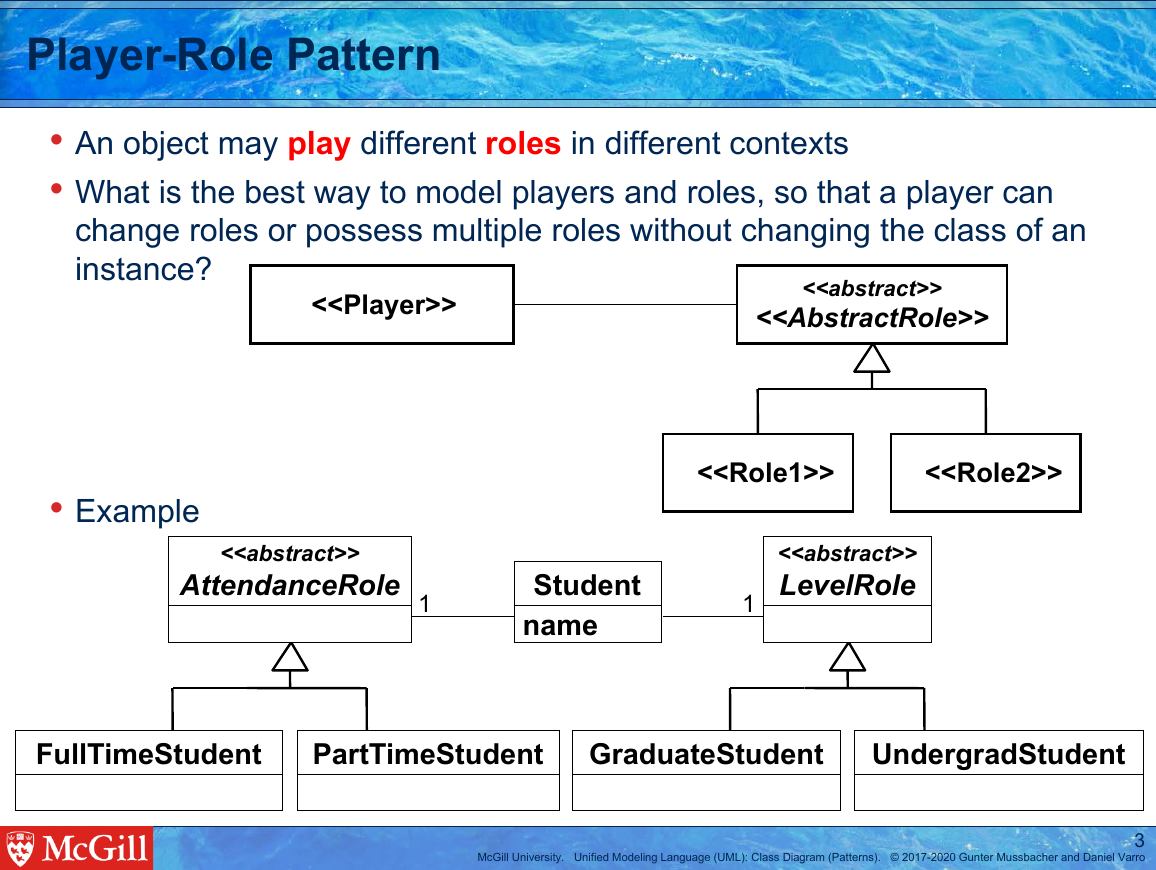
\includegraphics[width=0.6\textwidth]{images/player_role.png}
\end{tabular} \medskip


\subsubsection{Enumeration should be full Player-Role pattern}

\noindent Level 1: Highlight solution (Class) \medskip

\noindent Level 2: Text response: \medskip

\begin{tabular}{|p{0.9\linewidth}}
Think carefully about how to model the relationships between these concepts.
\end{tabular} \medskip

\noindent Level 3: Parametrized response: \medskip

\begin{tabular}{|p{0.9\linewidth}}
A \verb|${firstRole}| has different features from one of the other roles at the same time and different features need to be captured for the roles.
\end{tabular} \medskip

\noindent Level 4: Resource response with Quiz: \medskip


\begin{tabular}{lcccc}
\hline
\textbf{Solution} &
  \textbf{\begin{tabular}[c]{@{}c@{}}Roles\\ have\\ different\\ features\end{tabular}} &
  \textbf{\begin{tabular}[c]{@{}c@{}}Only one\\ role at\\ a time\end{tabular}} &
  \textbf{\begin{tabular}[c]{@{}c@{}}Different\\ roles\\ over time\end{tabular}} &
  \textbf{\begin{tabular}[c]{@{}c@{}}More than\\ one role\\ at the\\ same time\end{tabular}} \\ \hline
Enumeration         & $\square$   & $\boxtimes$ & $\boxtimes$ & $\square$   \\
Subclasses          & $\boxtimes$ & $\boxtimes$ & $\square$   & $\square$   \\
Associations        & $\square$   & $\boxtimes$ & $\boxtimes$ & $\boxtimes$ \\
Player-Role Pattern & $\boxtimes$ & $\boxtimes$ & $\boxtimes$ & $\boxtimes$ \\ \hline
\end{tabular} \bigskip


\noindent Level 5: Resource response with Reference: \medskip

\begin{tabular}{|p{0.9\linewidth}}
The Player-Role Pattern can be used to capture the fact that an object may play different roles
in different contexts.

\\
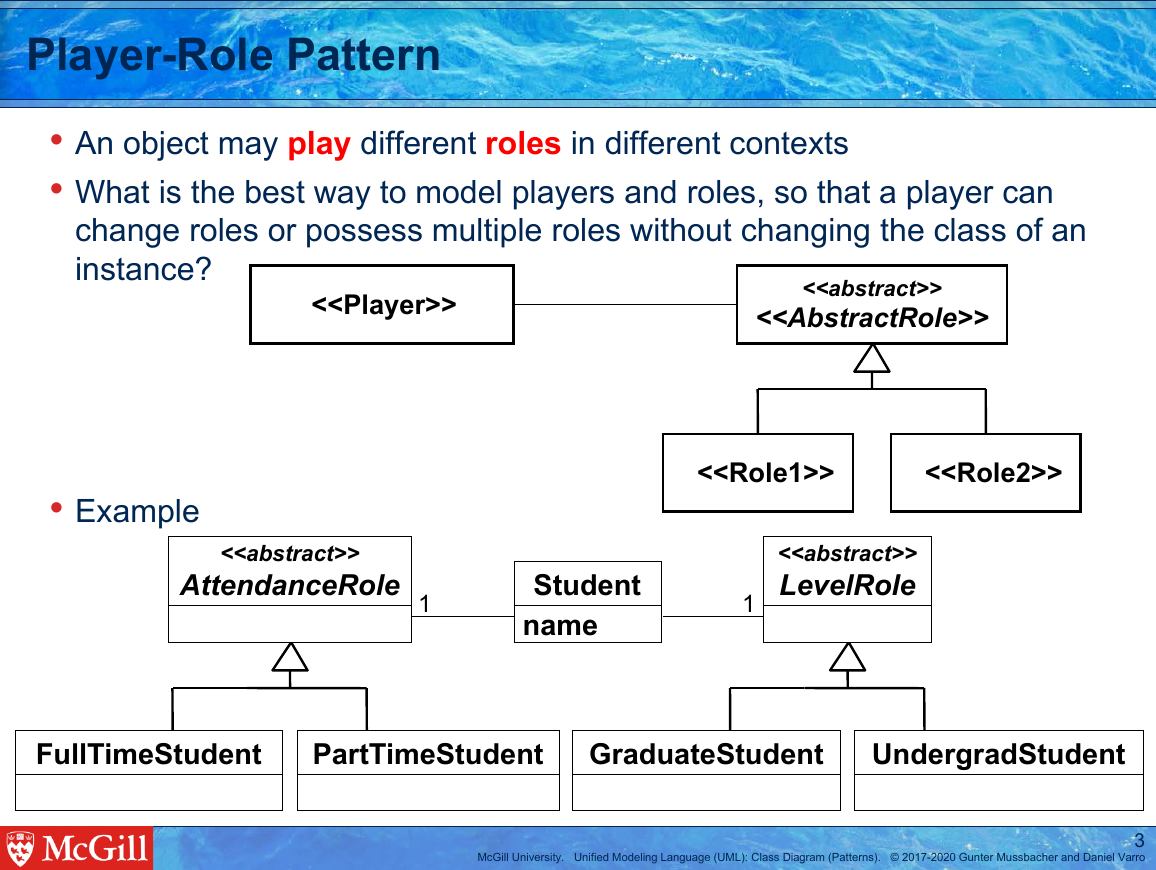
\includegraphics[width=0.6\textwidth]{images/player_role.png}
\end{tabular} \medskip


\subsubsection{Enumeration should be subclass Player-Role pattern}

\noindent Level 1: Highlight solution (Class) \medskip

\noindent Level 2: Text response: \medskip

\begin{tabular}{|p{0.9\linewidth}}
Think carefully about how to model the relationships between these concepts.
\end{tabular} \medskip

\noindent Level 3: Parametrized response: \medskip

\begin{tabular}{|p{0.9\linewidth}}
A \verb|${firstRole}| has different features from one of the other roles and this role never changes to another role.
\end{tabular} \medskip

\noindent Level 4: Resource response with Quiz: \medskip


\begin{tabular}{lcccc}
\hline
\textbf{Solution} &
  \textbf{\begin{tabular}[c]{@{}c@{}}Roles\\ have\\ different\\ features\end{tabular}} &
  \textbf{\begin{tabular}[c]{@{}c@{}}Only one\\ role at\\ a time\end{tabular}} &
  \textbf{\begin{tabular}[c]{@{}c@{}}Different\\ roles\\ over time\end{tabular}} &
  \textbf{\begin{tabular}[c]{@{}c@{}}More than\\ one role\\ at the\\ same time\end{tabular}} \\ \hline
Enumeration         & $\square$   & $\boxtimes$ & $\boxtimes$ & $\square$   \\
Subclasses          & $\boxtimes$ & $\boxtimes$ & $\square$   & $\square$   \\
Associations        & $\square$   & $\boxtimes$ & $\boxtimes$ & $\boxtimes$ \\
Player-Role Pattern & $\boxtimes$ & $\boxtimes$ & $\boxtimes$ & $\boxtimes$ \\ \hline
\end{tabular} \bigskip


\noindent Level 5: Resource response with Reference: \medskip

\begin{tabular}{|p{0.9\linewidth}}
The Player-Role Pattern can be used to capture the fact that an object may play different roles
in different contexts.

\\
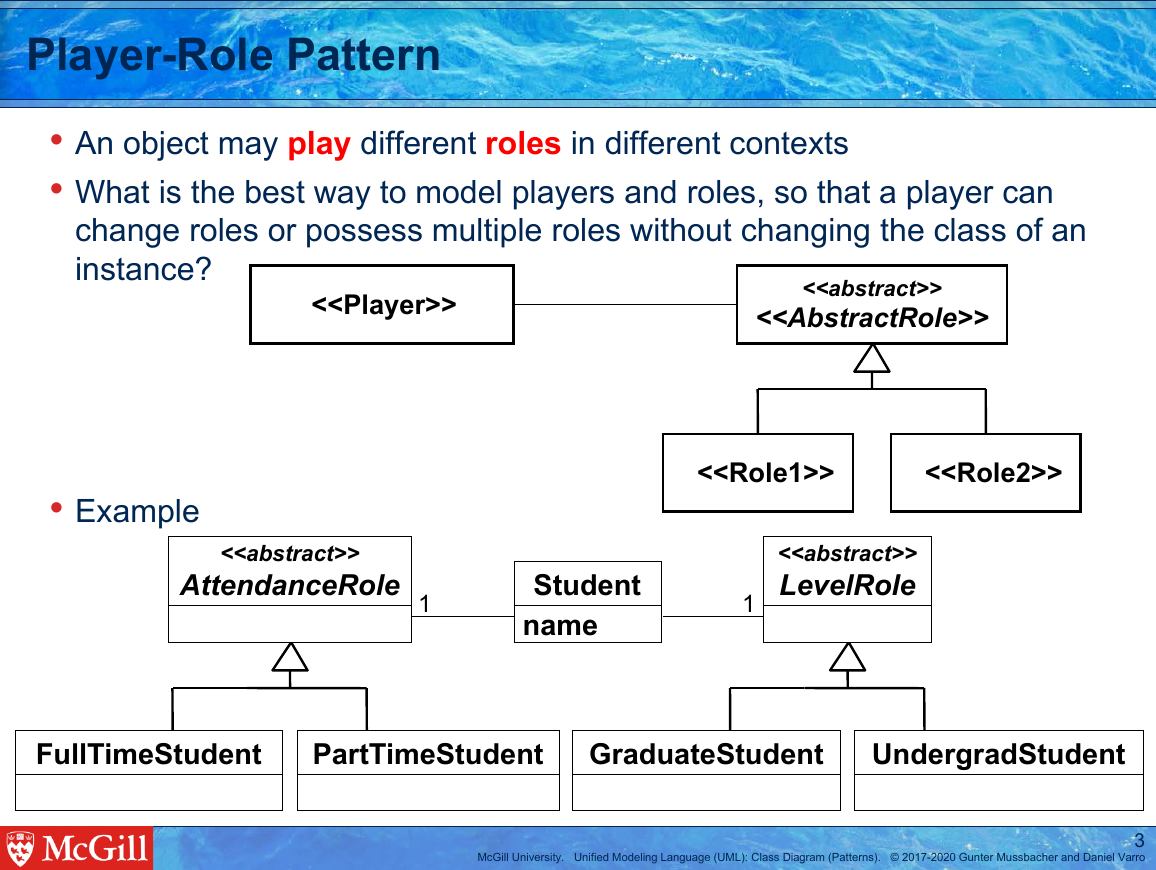
\includegraphics[width=0.6\textwidth]{images/player_role.png}
\end{tabular} \medskip


\subsubsection{Enumeration should be association Player-Role pattern}

\noindent Level 1: Highlight solution (Relationship) \medskip

\noindent Level 2: Text response: \medskip

\begin{tabular}{|p{0.9\linewidth}}
Think carefully about how to model the relationships between these concepts.
\end{tabular} \medskip

\noindent Level 3: Parametrized response: \medskip

\begin{tabular}{|p{0.9\linewidth}}
Will the roles of \verb|${firstRole}| and \verb|${secondRole}| ever be occupied at the same time?
\end{tabular} \medskip

\noindent Level 4: Resource response with Quiz: \medskip


\begin{tabular}{lcccc}
\hline
\textbf{Solution} &
  \textbf{\begin{tabular}[c]{@{}c@{}}Roles\\ have\\ different\\ features\end{tabular}} &
  \textbf{\begin{tabular}[c]{@{}c@{}}Only one\\ role at\\ a time\end{tabular}} &
  \textbf{\begin{tabular}[c]{@{}c@{}}Different\\ roles\\ over time\end{tabular}} &
  \textbf{\begin{tabular}[c]{@{}c@{}}More than\\ one role\\ at the\\ same time\end{tabular}} \\ \hline
Enumeration         & $\square$   & $\boxtimes$ & $\boxtimes$ & $\square$   \\
Subclasses          & $\boxtimes$ & $\boxtimes$ & $\square$   & $\square$   \\
Associations        & $\square$   & $\boxtimes$ & $\boxtimes$ & $\boxtimes$ \\
Player-Role Pattern & $\boxtimes$ & $\boxtimes$ & $\boxtimes$ & $\boxtimes$ \\ \hline
\end{tabular} \bigskip


\noindent Level 5: Resource response with Reference: \medskip

\begin{tabular}{|p{0.9\linewidth}}
The Player-Role Pattern can be used to capture the fact that an object may play different roles
in different contexts.

\\
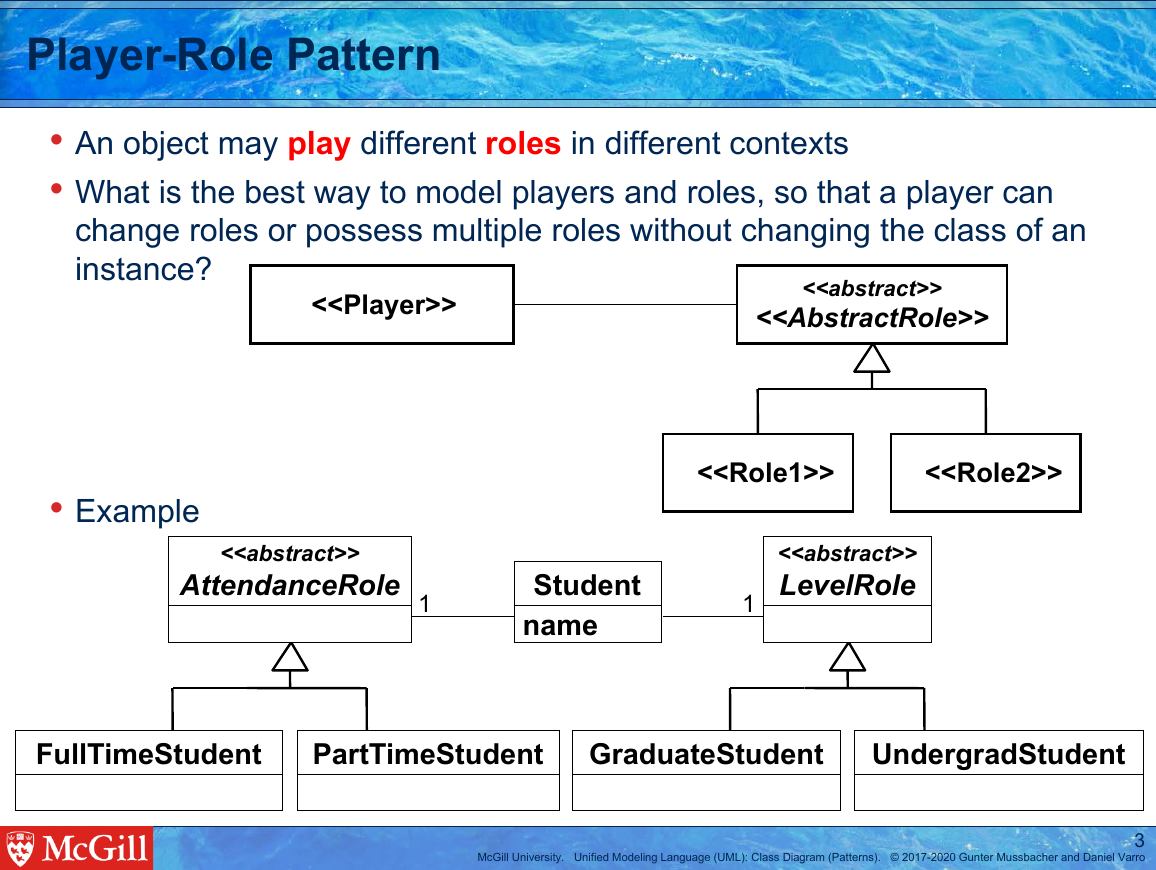
\includegraphics[width=0.6\textwidth]{images/player_role.png}
\end{tabular} \medskip


\subsubsection{Full Player-Role pattern should be subclass}

\noindent Level 1: Highlight solution (Class) \medskip

\noindent Level 2: Text response: \medskip

\begin{tabular}{|p{0.9\linewidth}}
Think carefully about how to model the relationships between these concepts.
\end{tabular} \medskip

\noindent Level 3: Parametrized response: \medskip

\begin{tabular}{|p{0.9\linewidth}}
Can a \verb|${firstRole}| can also play the role of one of the other roles at different times or at the same time?
\end{tabular} \medskip

\noindent Level 4: Resource response with Quiz: \medskip


\begin{tabular}{lcccc}
\hline
\textbf{Solution} &
  \textbf{\begin{tabular}[c]{@{}c@{}}Roles\\ have\\ different\\ features\end{tabular}} &
  \textbf{\begin{tabular}[c]{@{}c@{}}Only one\\ role at\\ a time\end{tabular}} &
  \textbf{\begin{tabular}[c]{@{}c@{}}Different\\ roles\\ over time\end{tabular}} &
  \textbf{\begin{tabular}[c]{@{}c@{}}More than\\ one role\\ at the\\ same time\end{tabular}} \\ \hline
Enumeration         & $\square$   & $\boxtimes$ & $\boxtimes$ & $\square$   \\
Subclasses          & $\boxtimes$ & $\boxtimes$ & $\square$   & $\square$   \\
Associations        & $\square$   & $\boxtimes$ & $\boxtimes$ & $\boxtimes$ \\
Player-Role Pattern & $\boxtimes$ & $\boxtimes$ & $\boxtimes$ & $\boxtimes$ \\ \hline
\end{tabular} \bigskip


\noindent Level 5: Resource response with Reference: \medskip

\begin{tabular}{|p{0.9\linewidth}}
The Player-Role Pattern can be used to capture the fact that an object may play different roles
in different contexts.

\\
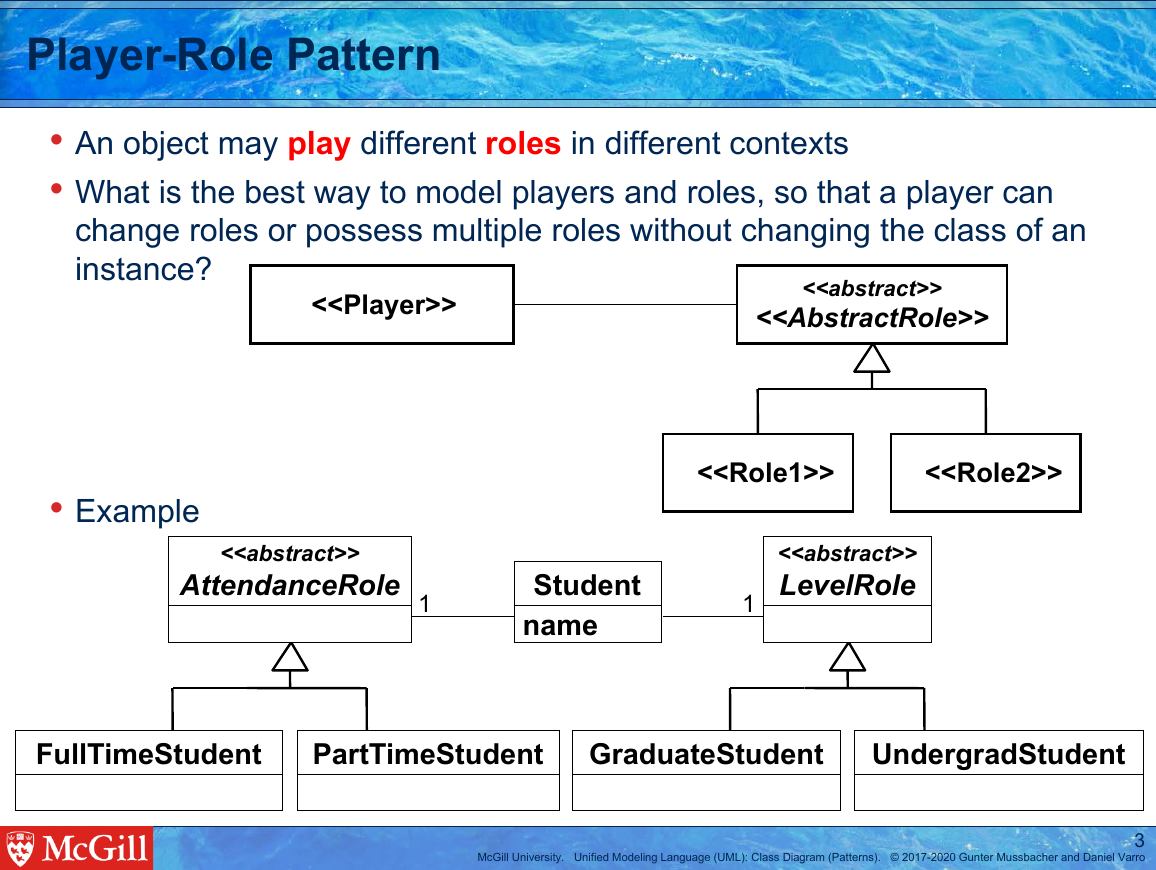
\includegraphics[width=0.6\textwidth]{images/player_role.png}
\end{tabular} \medskip


\subsubsection{Full Player-Role pattern should be association}

\noindent Level 1: Highlight solution (Relationship) \medskip

\noindent Level 2: Text response: \medskip

\begin{tabular}{|p{0.9\linewidth}}
Think carefully about how to model the relationships between these concepts.
\end{tabular} \medskip

\noindent Level 3: Parametrized response: \medskip

\begin{tabular}{|p{0.9\linewidth}}
Do \verb|${firstRole}| and \verb|${secondRole}| need to have different features?
\end{tabular} \medskip

\noindent Level 4: Resource response with Quiz: \medskip


\begin{tabular}{lcccc}
\hline
\textbf{Solution} &
  \textbf{\begin{tabular}[c]{@{}c@{}}Roles\\ have\\ different\\ features\end{tabular}} &
  \textbf{\begin{tabular}[c]{@{}c@{}}Only one\\ role at\\ a time\end{tabular}} &
  \textbf{\begin{tabular}[c]{@{}c@{}}Different\\ roles\\ over time\end{tabular}} &
  \textbf{\begin{tabular}[c]{@{}c@{}}More than\\ one role\\ at the\\ same time\end{tabular}} \\ \hline
Enumeration         & $\square$   & $\boxtimes$ & $\boxtimes$ & $\square$   \\
Subclasses          & $\boxtimes$ & $\boxtimes$ & $\square$   & $\square$   \\
Associations        & $\square$   & $\boxtimes$ & $\boxtimes$ & $\boxtimes$ \\
Player-Role Pattern & $\boxtimes$ & $\boxtimes$ & $\boxtimes$ & $\boxtimes$ \\ \hline
\end{tabular} \bigskip


\noindent Level 5: Resource response with Reference: \medskip

\begin{tabular}{|p{0.9\linewidth}}
The Player-Role Pattern can be used to capture the fact that an object may play different roles
in different contexts.

\\
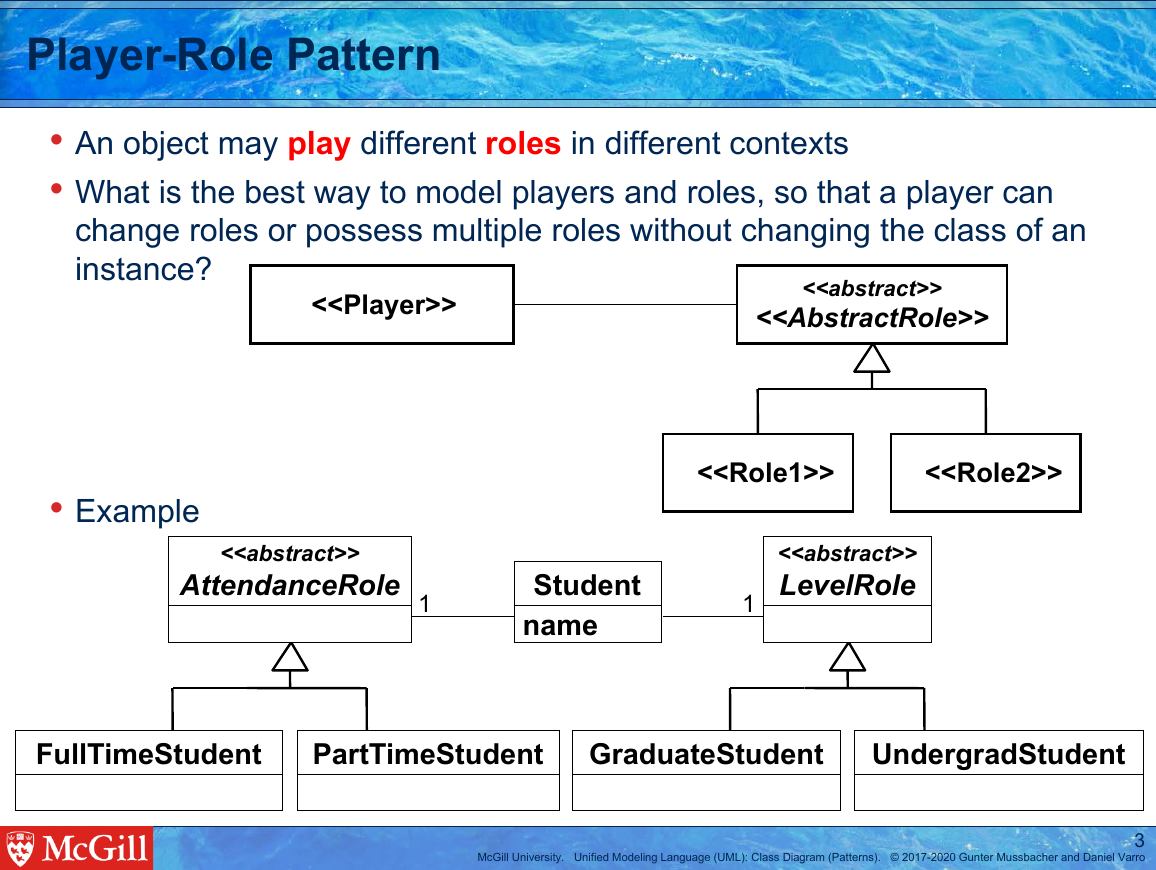
\includegraphics[width=0.6\textwidth]{images/player_role.png}
\end{tabular} \medskip


\subsubsection{Full Player-Role pattern should be enumeration}

\noindent Level 1: Highlight solution (Attribute) \medskip

\noindent Level 2: Text response: \medskip

\begin{tabular}{|p{0.9\linewidth}}
Think carefully about how to model the relationships between these concepts.
\end{tabular} \medskip

\noindent Level 3: Parametrized response: \medskip

\begin{tabular}{|p{0.9\linewidth}}
Do \verb|${firstRole}| and \verb|${secondRole}| need to have different features and is it possible that more than one role is played at the same time?
\end{tabular} \medskip

\noindent Level 4: Resource response with Quiz: \medskip


\begin{tabular}{lcccc}
\hline
\textbf{Solution} &
  \textbf{\begin{tabular}[c]{@{}c@{}}Roles\\ have\\ different\\ features\end{tabular}} &
  \textbf{\begin{tabular}[c]{@{}c@{}}Only one\\ role at\\ a time\end{tabular}} &
  \textbf{\begin{tabular}[c]{@{}c@{}}Different\\ roles\\ over time\end{tabular}} &
  \textbf{\begin{tabular}[c]{@{}c@{}}More than\\ one role\\ at the\\ same time\end{tabular}} \\ \hline
Enumeration         & $\square$   & $\boxtimes$ & $\boxtimes$ & $\square$   \\
Subclasses          & $\boxtimes$ & $\boxtimes$ & $\square$   & $\square$   \\
Associations        & $\square$   & $\boxtimes$ & $\boxtimes$ & $\boxtimes$ \\
Player-Role Pattern & $\boxtimes$ & $\boxtimes$ & $\boxtimes$ & $\boxtimes$ \\ \hline
\end{tabular} \bigskip


\noindent Level 5: Resource response with Reference: \medskip

\begin{tabular}{|p{0.9\linewidth}}
The Player-Role Pattern can be used to capture the fact that an object may play different roles
in different contexts.

\\
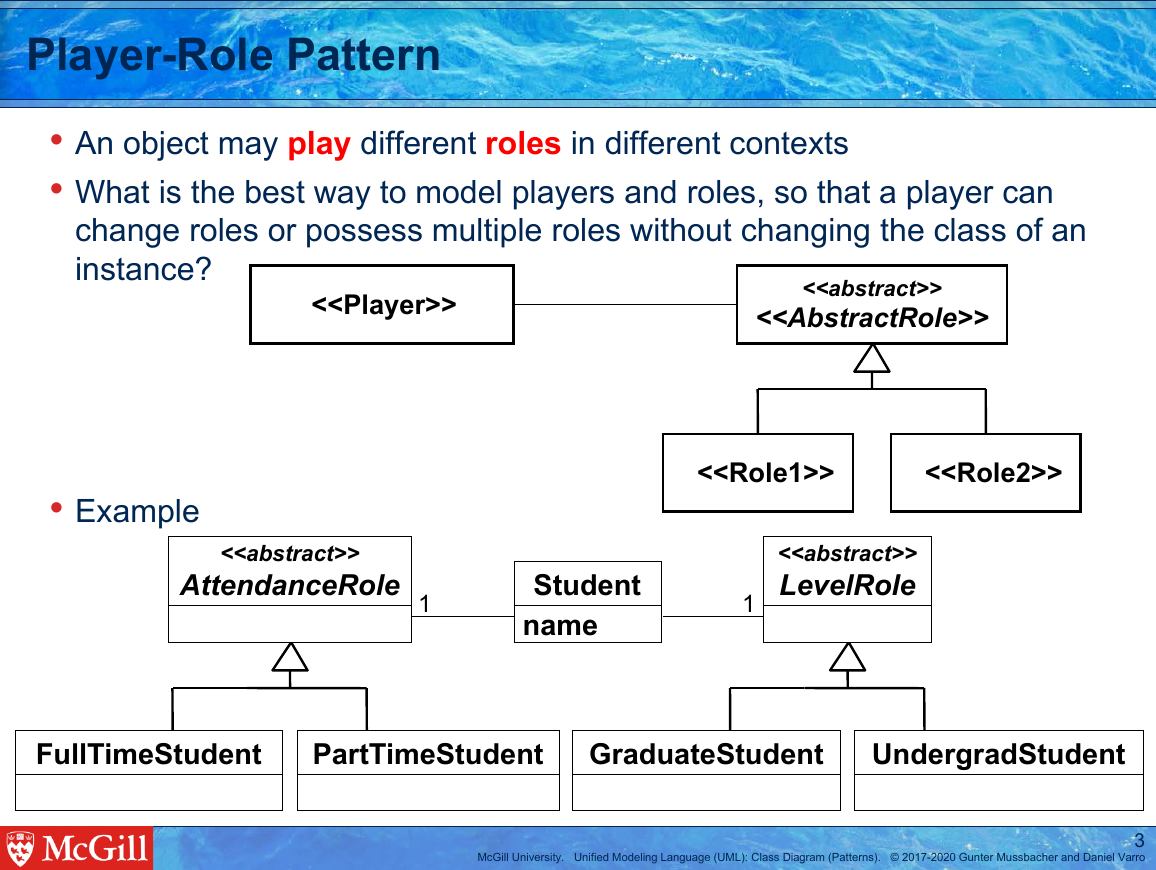
\includegraphics[width=0.6\textwidth]{images/player_role.png}
\end{tabular} \medskip


\subsection{Abstraction-Occurrence pattern mistakes}

\subsubsection{Missing Abstraction-Occurrence pattern}

\noindent Level 1: Highlight solution (Class) \medskip

\noindent Level 2: Text response: \medskip

\begin{tabular}{|p{0.9\linewidth}}
Think carefully about how to model the relationships between these concepts.
\end{tabular} \medskip

\noindent Level 3: Parametrized response: \medskip

\begin{tabular}{|p{0.9\linewidth}}
The concepts of \verb|${instructorAbstraction}| and \verb|${instructorOccurrence}| and the relationship between them should be modeled with the Abstraction-Occurrence pattern.
\end{tabular} \medskip

\noindent Level 4: Resource response with Reference: \medskip

\begin{tabular}{|p{0.9\linewidth}}
The \textit{Abstraction-Occurrence Pattern} can be used to 
represent a set of related objects that share common information but also differ
from each other in an important way.

\\
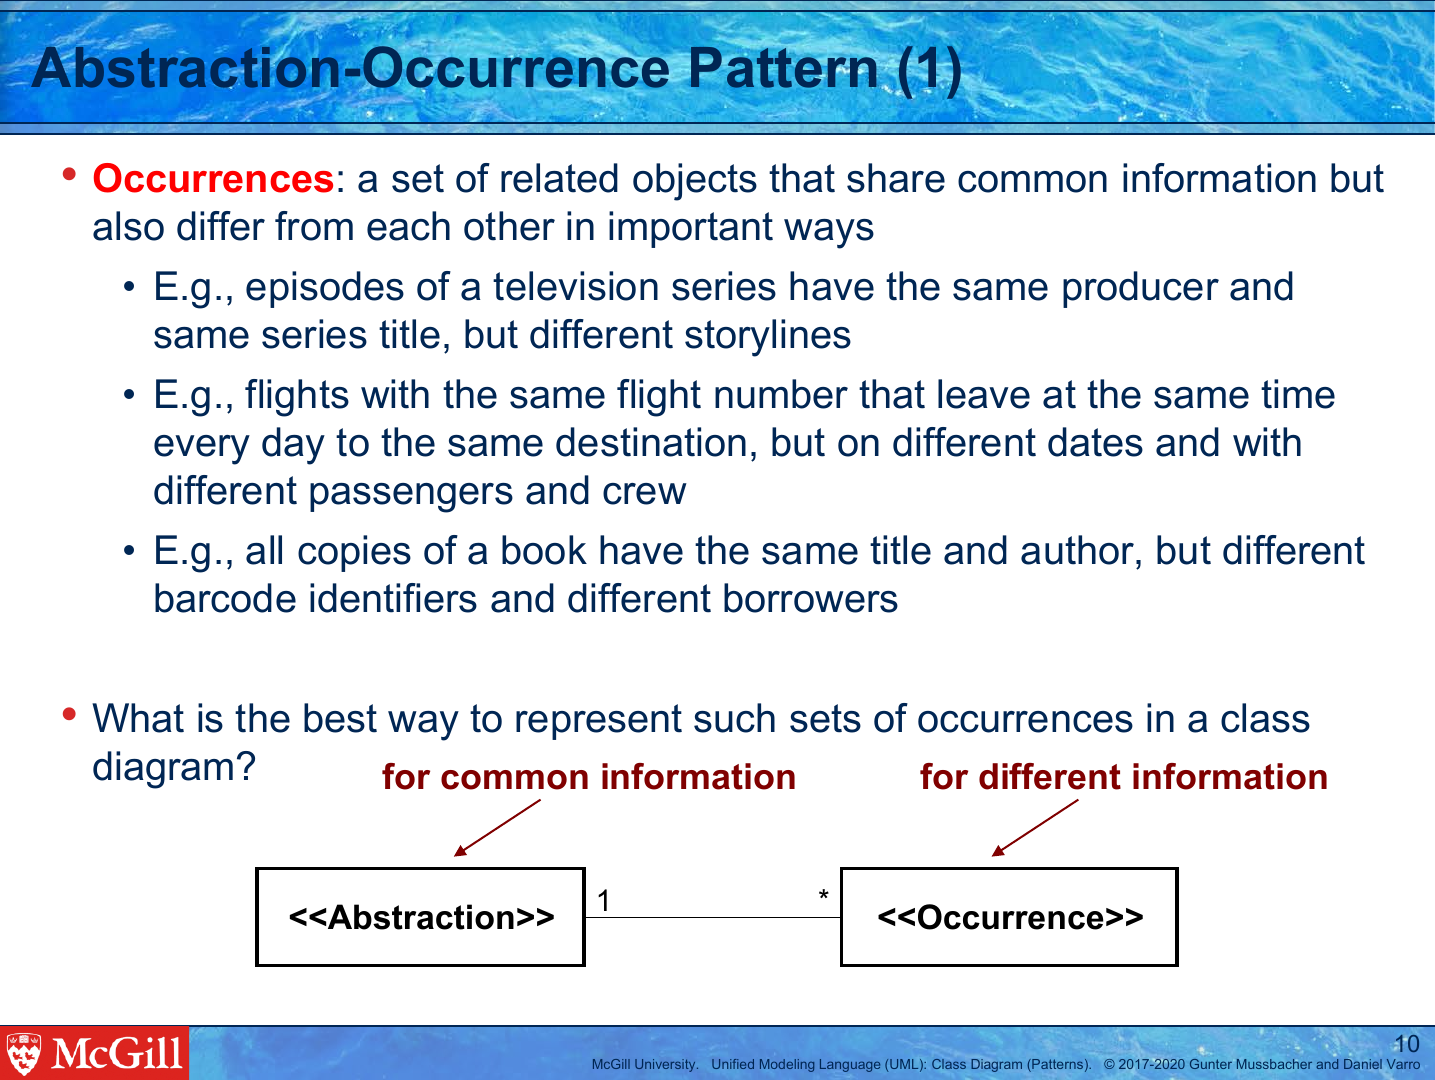
\includegraphics[width=0.6\textwidth]{images/abstraction_occurrence.png}
\end{tabular} \medskip


\subsubsection{Incomplete Abstraction-Occurrence pattern}

\noindent Level 1: Highlight solution (Class) \medskip

\noindent Level 2: Text response: \medskip

\begin{tabular}{|p{0.9\linewidth}}
Think carefully about how to model the relationships between these concepts.
\end{tabular} \medskip

\noindent Level 3: Parametrized response: \medskip

\begin{tabular}{|p{0.9\linewidth}}
The concepts of \verb|${instructorAbstraction}| and \verb|${instructorOccurrence}| and the relationship between them should be modeled with the Abstraction-Occurrence pattern.
\end{tabular} \medskip

\noindent Level 4: Resource response with Reference: \medskip

\begin{tabular}{|p{0.9\linewidth}}
The \textit{Abstraction-Occurrence Pattern} can be used to 
represent a set of related objects that share common information but also differ
from each other in an important way.

\\
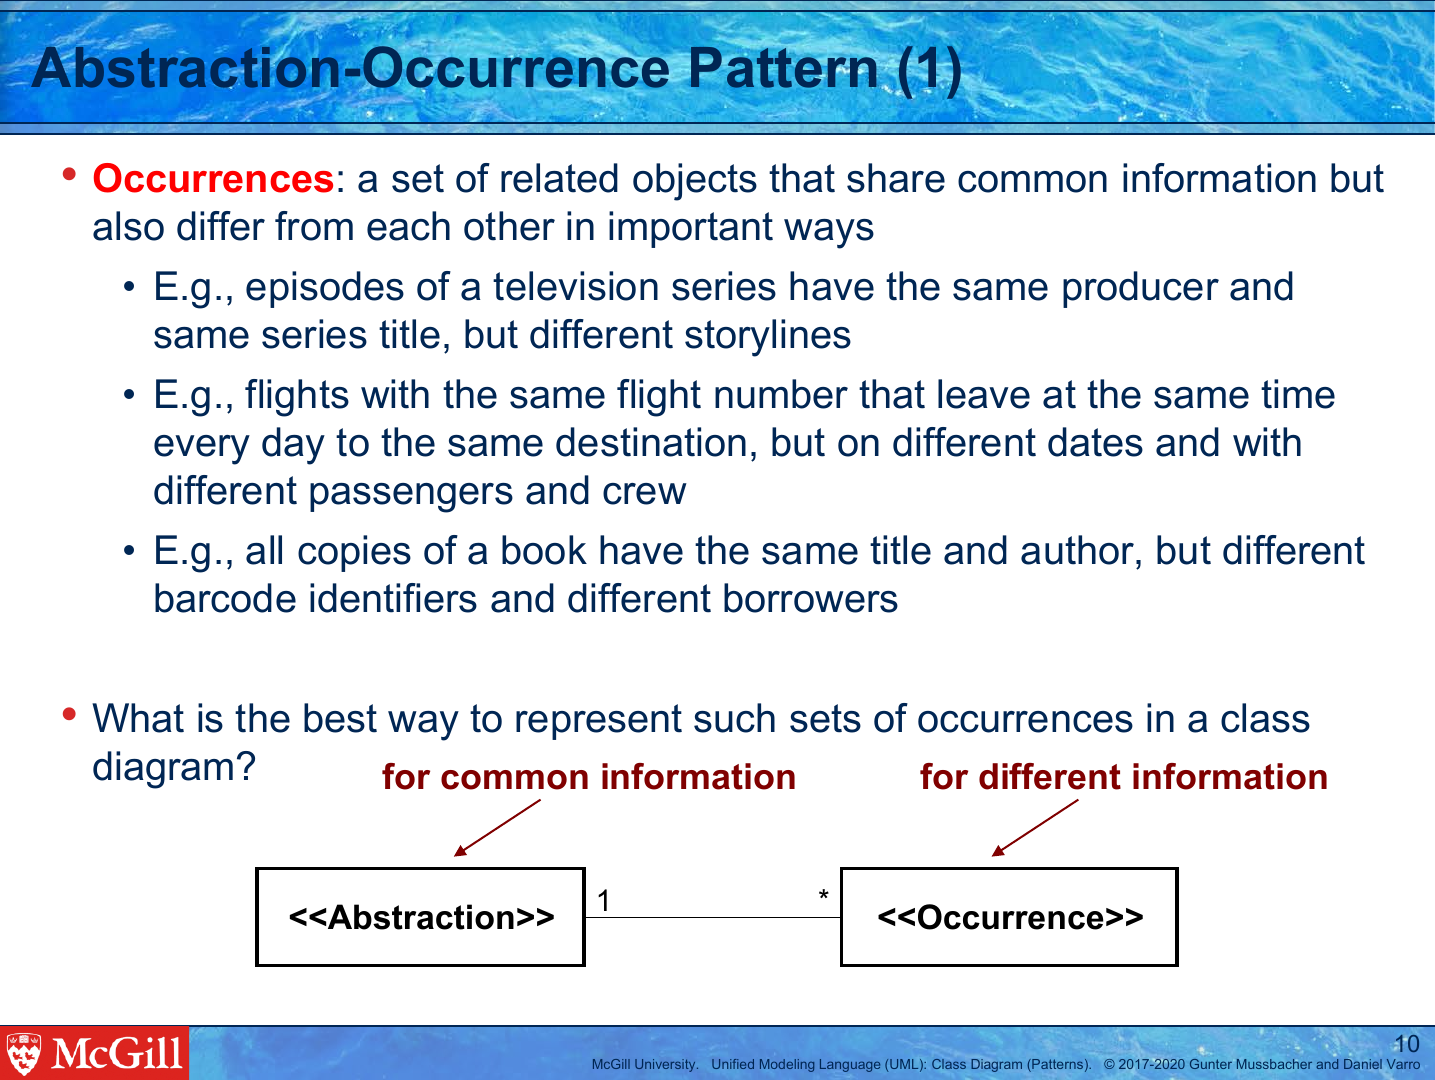
\includegraphics[width=0.6\textwidth]{images/abstraction_occurrence.png}
\end{tabular} \medskip


\subsubsection{Generalization should be association in Abstraction-Occurrence pattern}

\noindent Level 1: Highlight solution (Class) \medskip

\noindent Level 2: Text response: \medskip

\begin{tabular}{|p{0.9\linewidth}}
Think carefully about how to model the relationships between these concepts.
\end{tabular} \medskip

\noindent Level 3: Text response: \medskip

\begin{tabular}{|p{0.9\linewidth}}
Is generalization the correct way to model this use of the Abstraction-Occurrence pattern?
\end{tabular} \medskip

\noindent Level 4: Resource response with Reference: \medskip

\begin{tabular}{|p{0.9\linewidth}}
The \textit{Abstraction-Occurrence Pattern} can be used to 
represent a set of related objects that share common information but also differ
from each other in an important way.

\\
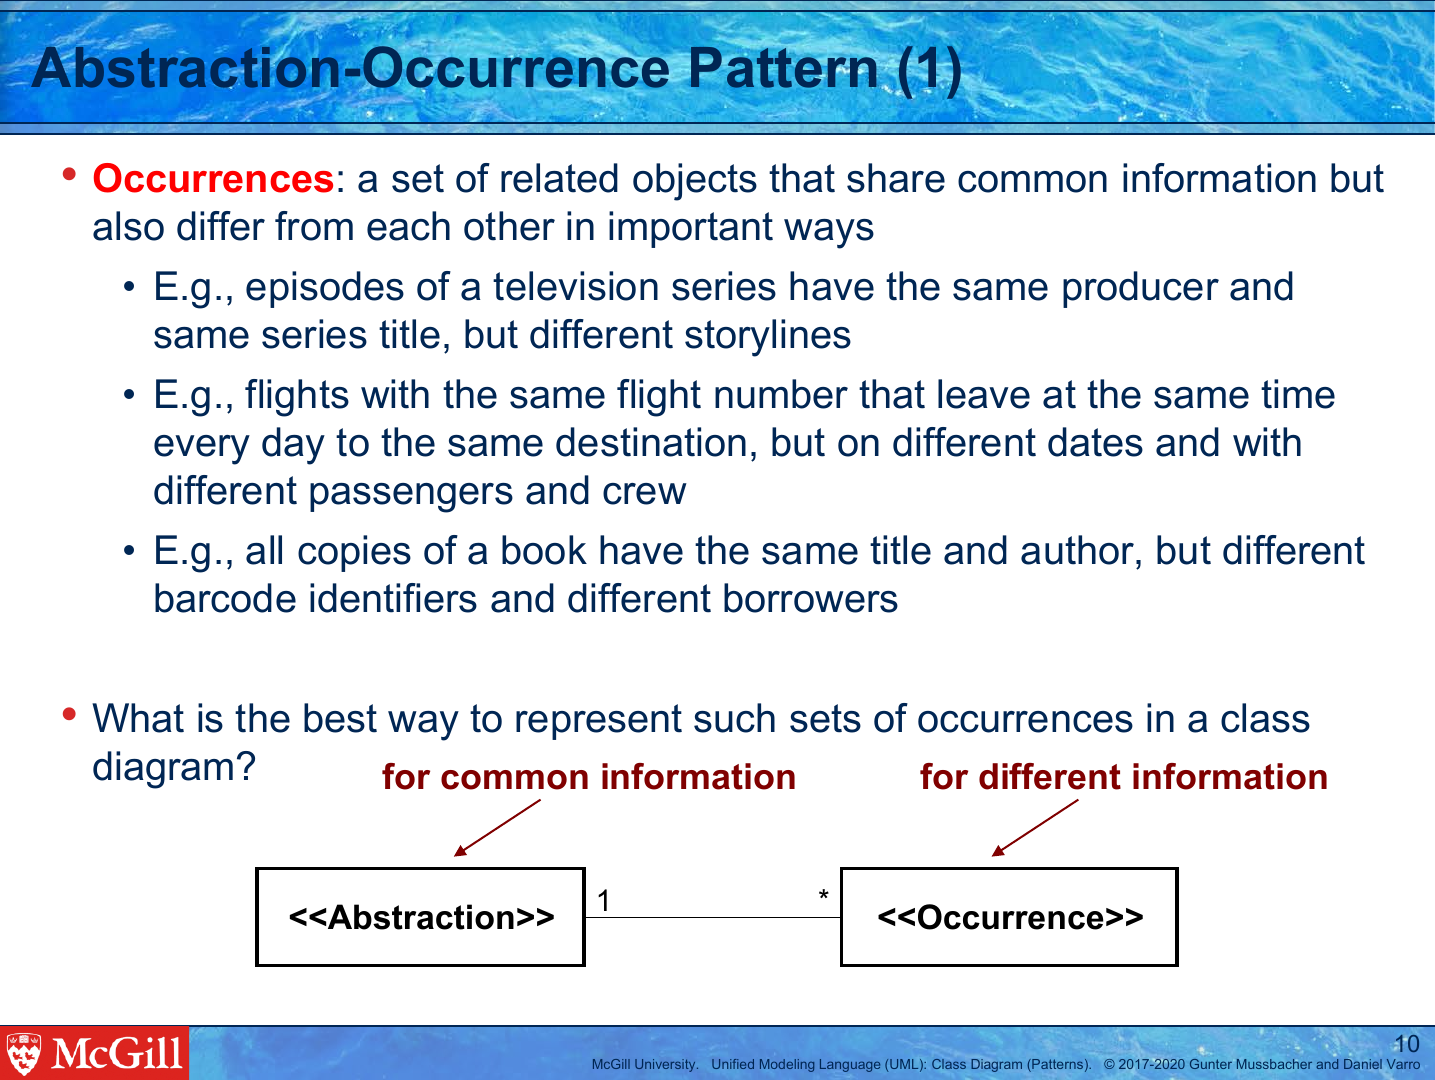
\includegraphics[width=0.6\textwidth]{images/abstraction_occurrence.png}
\end{tabular} \medskip



